\deelzonderoef{Module 2}{Elementaire rekenvaardigheden B}{Module 2. Elementaire rekenvaardigheden B}

\section*{Intro}

\begin{minipage}{.25\linewidth}
	\raggedright
	
\includegraphics[width=4cm]{2_elem_rekenvaardigheden_B/inputs/QR_Code_INTRO_module2new}
\end{minipage}
\begin{minipage}{.7\linewidth}
	Zie filmpje MOOC.
\end{minipage}

\section{Functies}

%\subsection{Re\"ele functies}

\subsubsection{Definitie, notatie, functievoorschrift}

\begin{definitie}
	
Een functie is een verband: een functie $f$  associeert bij elk gegeven getal $x$ hoogstens \'e\'en ander getal (de functiewaarde $f(x)$). De functie $f$ kan een functievoorschrift hebben om volgens een bepaalde vaste regel van zo'n $x$ de bijhorende functiewaarde $f(x)$ te berekenen.

\end{definitie}

Er zijn functies met een speciale naam, zoals de sinus-functie: $\sin$ en functies met speciale symbolen, zoals de wortel-functie: $\sqrt{\ }$. Het functievoorschrift van deze functies is resp. $f(x)=\sin(x)$ en $f(x)=\sqrt{x}$.

\subsubsection{Grafische voorstelling}

\begin{definitie}
	Een functie $f$  kan altijd grafisch worden weergeven. De vergelijking $f=f(x)$  geeft het verband tussen de $x$-waarden op de \emph{horizontale} as en de functiewaarden $f(x)$ op de \emph{verticale} as.
\end{definitie}

De letter $y$ wordt de \emph{afhankelijke variabele}, de
\emph{beeldwaarde} (of kortweg het \emph{beeld}), de \emph{output}
of ook nog de \emph{functiewaarde} genoemd. 
De letter $x$ is hier
de \emph{onafhankelijke variabele}, de \emph{input} of ook wel het
\emph{argument} genoemd. 

Voorbeeld: het verband tussen de temperatuur in graden
Celsius \textdegree$C$ ($x$) en graden Fahrenheit \textdegree$F$ ($y$)
wordt gegeven door volgende functie: $y=1,8x+32$

%Merk op dat bij een functie voor elke $y$-waarde hoogstens
%één $x$-waarde mag bestaan. M.a.w. met niet elke $x$-waarde hoeft
%een beeldwaarde $y$ overeen te komen, maar als er een beeld is, mag
%er slechts één beeld zijn. Als er meerdere beelden bestaan spreken
%we van een \emph{relatie}.


\subsubsection{Domein en beeld}


\begin{definitie}
	Het \emph{domein} (of \emph{definitiegebied}) van een functie
$f$ is de verzameling van alle getallen $\in \mathbb{R}$ ($x$-waarden) die en beeld
een beeld ($y$-waarde) hebben. Het domein is dus de
verzameling van alle getallen $\in \mathbb{R}$ die acceptabel zijn als input.
\end{definitie}
\begin{notatie}
$\textrm{dom}f$ of $\textrm{def}f$.
\end{notatie}



\begin{voorbeeld}
	Voor de functie $y=\sqrt{x}$ mag $x$ geen
negatief getal zijn, dus $\textrm{dom}f=\mathbb{R}^{+}=\left[0,+\infty\right[$
\end{voorbeeld}

\begin{voorbeeld}
	De functie $y=\frac{1}{x-1}$ heeft geen beeld
voor $x=1$, dus $\textrm{dom}f=\mathbb{R}\setminus\left\{ 1\right\} $

\end{voorbeeld}

Tips bij het bepalen van het domein:
\begin{itemize}
\item Een even machtswortel kan je enkel nemen van positieve getallen $\in \mathbb{R}$.
\item Een oneven machtswortel kan je van elk getal $\in \mathbb{R}$ nemen.
\item Delen door nul mag niet!
\end{itemize}

\begin{definitie}
	Het \emph{beeld} (of \emph{bereik}) van een functie $f$
is de verzameling van alle getallen $\in \mathbb{R}$ welke het beeld (de functiewaarde
$y$) van de functie kunnen zijn. Het beeld is dus de verzameling
van alle getallen $\in \mathbb{R}$ die kunnen optreden als output. Notatie: $\textrm{bld}f$.
\end{definitie}

Merk op dat bij een functie voor elke beeldwaarde hoogstens 1 $x$-waarde mag bestaan.

Bij een vergelijking waarbij er meerdere beelden bestaan voor een $x$-waarde, spreken we van een relatie.

\begin{ftonthoud}
\begin{itemize}
\item Het domein lees je af op de horizontale $x$-as (in onderstaande voorbeelden aangeduid met een groene lijn).
\item Het beeld lees je af op de verticale $y$-as (in onderstaande voorbeelden aangeduid met een blauwe lijn).
\end{itemize}
\end{ftonthoud}


\begin{voorbeeld}
Bij de functie $f(x)=1-x^{2}$ kan je voor geen
enkele waarde van $x$ een beeldwaarde bekomen die groter is dan 1 (omdat $1-x^2 \le 1$),
dus $\textrm{bld}f=\left]-\infty,1\right]$
\end{voorbeeld}

De vergelijking $y^2=x$ kunnen we niet zien als een functie in $x$, omdat zowel $y=1$ als $y=-1$ zouden horen bij $x=1$. Dit is dus een voorbeeld van een relatie (maar geen functie)!

\subsubsection{Nulpunten}

\begin{definitie}
	Een \emph{nulwaarde} van de functie $f$ is een getal $a$ waarvoor geldt dat $f(a)=0$. Het punt $(a,0)$ noemen we een nulpunt.
\end{definitie}

Het berekenen van de nulwaarden van een
functie $f$ vereist het oplossen van de vergelijking $f(x)=0$.
Grafisch gezien zijn de nulpunten $(a,0)$ de snijpunten van de grafiek
van de functie $f$ met de horizontale as (de $X$-as).

\begin{voorbeeld}
	Voor de tweedegraadsfunctie met voorschrift $f(x)=ax^2+bx+c$ komt dit neer op $ax^2+bx+c=0$ oplossen en kunnen we dus de methode van de discriminant toepassen om de nulwaarden te vinden.
\end{voorbeeld}

\subsubsection{Snijpunten met de assen}

De snijpunten van de functie $f$ met de $x$-as vinden
we door het oplossen van het stelsel
\begin{equation*}
\begin{cases}
y=f(x)\\
y=0
\end{cases}
\end{equation*}


 of dus de vergelijking $f(x)=0$. Het snijpunt van de functie $y=f(x)$ met de $y$-as vinden
we door het oplossen van het stelsel 
$\begin{cases}
y=f(x)\\
x=0
\end{cases}$ of dus het berekenen van $f(0)$.


%\subsubsection{Grafische voorstelling}
%
%Een functie $y=f(x)$ kan altijd grafisch worden weergeven.
%Voor een functie $y=f(x)$ staan de $x$-waarden op de horizontale
%as en de functiewaarden $f(x)$ op de verticale as.
%
%Het domein lees je af op de horizontale $X$-as (in onderstaande
%voorbeelden aangeduid met een groene lijn) 
%
%Het beeld lees je af op de verticale $Y$-as (in onderstaande
%voorbeelden aangeduid met een blauwe lijn)


\subsubsection{Even en oneven functies}


\begin{definitie}
	Een functie $f(x)$ noemt men \emph{even} als $f(-x)=f(x)$.
\\
Een even functie heeft de $y$-as als as van symmetrie.


Een functie $f(x)$ noemt men \emph{oneven} als $f(-x)=-f(x)$.
\\
Een oneven functie heeft de oorsprong als middelpunt van symmetrie.

\end{definitie}

Als voor een functie $f(-x)$ niet gelijk is aan $f(x)$
of $-f(x)$ dan is de functie noch even, noch oneven. Dit hoeft niet
te betekenen dat deze functie niet ergens anders symmetrisch zou kunnen
zijn.




\begin{voorbeeld}
	De functie $f$ met voorschrift $f(x)=x^2$ is een eenvoudig voorbeeld van een even functie. Voor elke  $x \in \mathbb{R}$ geldt immers dat 

\begin{equation*}
f(-x)=(-x)^2=x^2=f(x)
\end{equation*}

De functie $g$ met voorschrift $g(x)=x^3$ is dan weer een eenvoudig voorbeeld van een oneven functie. Voor elke $x \in \mathbb{R}$ geldt immers dat

\begin{equation*}
g(-x)=(-x)^3=-x^3=g(x)
\end{equation*}

Een functie $h$ met voorschrift $h(x)=x+1$ is noch een even functie, noch een oneven functie. Er zijn namelijk $x$-waarden waarvoor geen van de verbanden gelden:

\begin{eqnarray*}
h(1) = 2 &\text{ maar }& h(-1) = 0 \\
h(2) = 3 &\text{ maar }& h(-2) = -1 
\end{eqnarray*}

\end{voorbeeld}

\subsubsection{Snijpunten van twee functies}

Als je voor twee verschillende functies $f$ en $g$ de
eventuele snijpunten van hun grafiek zoekt, dan moet je de vergelijking
$f(x)=g(x)$ oplossen. Zo vind je de $x$-co\"ordinaten van de snijpunten.


Invullen van deze gevonden $x$-co\"ordinaten in één van de twee functievoorschriften
geeft dan de bijhorende $y$-co\"ordinaten.




\begin{voorbeeld}
	Om te bepalen waar de snijpunten van de grafieken van $f(x)=x^2$ en $g(x)=3x-2$ liggen, onderzoeken we bijgevolg

\begin{equation*}
x^2 = 3x-2 \iff x^2-3x+2=0
\end{equation*}

wat snel opgelost kan worden met de methode van de discriminant:

\begin{equation*}
D = b^2 - 4ac = 9-8=1
\end{equation*}

zodat

\begin{equation*}
x_1 = \frac{3+1}{2} \text{ en } x_2 = \frac{3-1}{2} = 1.
\end{equation*}


De snijpunten van de grafieken van $f$ en $g$ hebben dus als $x$-waarden 1 en 2. Ook de beeldwaarden van deze snijpunten kunnen we nu snel berekenen: $f(1)=1$ en $f(2)=4$.

\end{voorbeeld}

%Opmerking 1: eigenlijk hebben we dit reeds toegepast om
%de nulpunten van een functie te vinden (= snijpunten met de $X$-as).
%Hierbij is dan de functie $g(x)=0$.
%
%
%
%
%Opmerking 2: een vaak voorkomend probleem is het vinden
%van de (twee) nulpunten van de tweedegraadsvergelijking $f(x)=ax^{2}+bx+c$
%of m.a.w. zoek de snijpunten van deze parabool met de $X$-as. De
%oplossingen $x_{1}$ en $x_{2}$ van de vergelijking $f(x)=ax^{2}+bx+c=0$
%kunnen snel gevonden worden via de formules $x_{1}=\frac{-b+\sqrt{b^{2}-4ac}}{2a}$
%en $x_{2}=\frac{-b-\sqrt{b^{2}-4ac}}{2a}$



%\subsection{Voorbeelden}

\begin{voorbeeld}
	Bespreek de functie $f$ met voorschrift $f(x)=\sqrt{10-2x}-2$.

%\begin{figure}[h]
	%\centering{}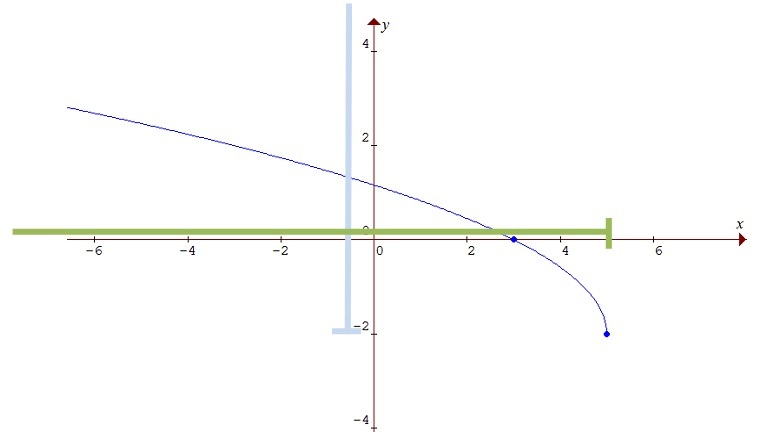
\includegraphics[height=5cm]{2_elem_rekenvaardigheden_B/inputs/reeel_vb1.jpg} 
%\end{figure}

%TODO figuur inladen 
\begin{figure}
	\centering          
	\tikzsetfigurename{Fig_module_2_1_2_reele_functies_vb1}
%TODO polynoombenadering uitrekenen > zie cursus Algebra

\begin{tikzpicture}[cap=round]

% Styles
\tikzstyle{axes}=[]
\tikzstyle help lines=[color=blue!50,very thin,dotted]


%%%%%%%%%%%%%%%%%%%%%%%%%%%%%%%%
%		GRID
%%%%%%%%%%%%%%%%%%%%%%%%%%%%%%%%

\draw[style=help lines,step=1cm] (-6.9,-3.9) grid (6.9,3.9);



%%%%%%%%%%%%%%%%%%%%%%%%%%%%%%%%
%		ASSENSTELSEL
%%%%%%%%%%%%%%%%%%%%%%%%%%%%%%%%

\draw[->] (-7,0) -- (7,0) node[right] {$x$};
\draw[->] (0,-4) -- (0,4) node[left]{$y$};

%\draw[fill,cyan](1,1)circle [radius=0.025];

%\draw[red,cap=rect, loosely dashed, ultra thick, domain=-2:2] plot (\x, {(\x*\x-1)+0.05}) node[above,yshift=-.7cm, right]{};

%%%%%%%%%%%%%%%%%%%%%%%%%%%%%%%%
%legende
%%%%%%%%%%%%%%%%%%%%%%%%%%%%%%%%
%\tkzDefPoint(0.5,3.5){A}
%\tkzDefPoint(1,3.5){B}
%\tkzLabelPoint[right,xshift=+0.1cm](B){${\color{cyan}f(x)=|x^2-1|}$}
%\tkzDrawSegment[cyan,ultra thick](A,B)

%\tkzDefPoint(0.5,3.2){C}
%\tkzDefPoint(1,3.2){D}
%\tkzLabelPoint[right,xshift=+0.1cm](D){${\color{red}e(x)=x^2-1}$}
%\tkzDrawSegment[red,cap=rect, loosely dashed, ultra thick](C,D)


%%%%%%%%%%%%%%%%%%%%%%%%%%%%%%%%
%getallen op de x-as en lijntjes
%%%%%%%%%%%%%%%%%%%%%%%%%%%%%%%%   
\foreach \x/\xtext in {-6,-5,-4,-3,-2,-1,1,2,3,4,5,6}
	\draw[xshift=\x cm] (0pt,1pt) -- (0pt,0pt) node[below,fill=white]
	{$\xtext$};,3
	
%getallen op de y-as en lijntjes  
%BEGIN LUS
\foreach \y/\ytext in {-4,-3,-2,-1,1,2,3}
	\draw[yshift=\y cm] (1pt,0pt) -- (0pt,0pt) node[left,fill=white]
	{$\ytext$}; %EINDE LUS



%%%%%%%%%%%%%%%%%%%%%%%%%%%%%%%%
%		GRAFIEKEN
%%%%%%%%%%%%%%%%%%%%%%%%%%%%%%%%
%\draw[cyan,cap=rect,thick, domain=-6:6] plot (\x, \x) node[above, right]{${\color{cyan}y=x}$};v

%\draw[cyan,cap=rect,ultra thick, domain=-6:1.75] plot (\x, {(\x-2)^(-1)}) node[above,right]{};


%\draw[cyan,cap=rect,ultra thick, domain=2.25:6] plot (\x, {(\x-2)^(-1)}) node[above,yshift=+0.5cm,left]{$\color{cyan} y=\frac{1}{x-2}$};


%\draw[cyan,cap=rect,ultra thick, domain=-7:1.9] plot (\x, {exp{\x}}) node[above, right]{${\color{cyan}y=\exp{x}}$};

%%%%%%%%%%%%%%%%%%%%%%%%%%%%%%%%
%		MARKERINGEN
%%%%%%%%%%%%%%%%%%%%%%%%%%%%%%%%
%verticale lijn
\draw[-o,line width=4,teal, cap=rect,opacity=0.3] (0,-4) -- (0,0.25) node[right] {};
\draw[line width=4,teal, cap=rect,opacity=0.3] (0,0) -- (0,4.2) node[right] {bld $f$ = $\mathbb{R}_0$};
%horizontale lijn
\draw[arrows=-o,line width=4,blue, cap=rect,opacity=0.3] (-7,0) -- (2.25,0) node[right] {};
\draw[line width=4,blue, cap=rect,opacity=0.3] (2.25,0) -- (7,0) node[below,yshift=-0.3cm] {dom$f$ = $\mathbb{R}  \setminus 2 $};
 
\end{tikzpicture}

	\caption{voorbeeld 1}
\label{fig:reele_functies_vb1}	
\end{figure}



\textbf{Domein}: de uitdrukking onder de vierkantswortel
mag niet negatief worden:


\begin{eqnarray*}
	\begin{array}{cccc}
		& 10-2x & \geqslant & 0\\
		\iff & 10 & \geqslant & 2x\\
		\iff & 5 & \geqslant & x\\
		\iff & x & \leqslant & 5
	\end{array}
\end{eqnarray*}


Besluit: voor $x$ zijn alle waarden van $-\infty$ tot
en met $5$ toegelaten. We schrijven: $\textrm{dom}\ f(x)=]-\infty,5]$ 

\textbf{Beeld}: de kleinste functiewaarde wordt
bekomen als de wortel $0$ is. Vierkantwortels geven altijd een positief
resultaat (of nul). De uitdrukking onder de wortel wordt $0$ als
$x=5$. We zien dat $f(5)=-2$. Er is geen bovengrens, dus het bereik
loopt tot $+\infty$.

Besluit: $\textrm{bld}f=[-2,+\infty[$




\textbf{Nulpunten}: voor welke waarden van $x$ wordt $f(x)=0$?


\begin{eqnarray*}
	\begin{array}{cccc}
		& \sqrt{10-2x}-2 & = & 0\\
		\iff & \sqrt{10-2x} & = & 2\\
		\iff & \left(\sqrt{10-2x}\right)^{2} & = & 2^{2}\\
		\iff & 10-2x & = & 4\\
		\iff & 6 & = & 2x\\
		\iff & x & = & 3
	\end{array}
\end{eqnarray*}


Besluit: er is slechts 1 nulwaarde, en dit is $x=3$ .




\textbf{Symmetrie}: we gaan na of het beeld van $-x$ hetzelfde
of het tegengestelde resultaat geeft als de gegeven functie. $f(-x)=\sqrt{10-2(-x)}-2=\sqrt{10+2x}-2$.
Dit is noch gelijk aan $f(x)$ noch gelijk aan $-f(x)$. Deze functie
is dus noch even, noch oneven.

\end{voorbeeld}

\begin{voorbeeld}
	Bespreek de functie met voorschrift $f(x)=\frac{1}{x-2}$.

%\begin{figure}[h]
%	\centering{}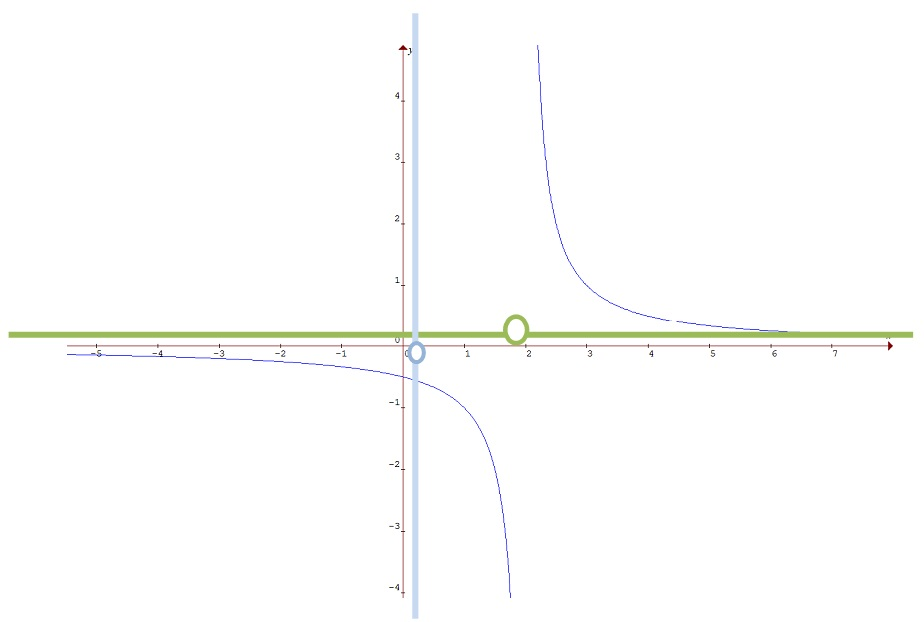
\includegraphics[height=5cm]{2_elem_rekenvaardigheden_B/inputs/reeel_vb2.jpg} 
%\end{figure}

%TODO figuur inladen

\begin{figure}
	\centering          
	
\begin{center}
\begin{tikzpicture}[scale=1,cap=round]

% Styles
\tikzstyle{axes}=[]
\tikzstyle help lines=[color=blue!50,very thin,dotted]


%%%%%%%%%%%%%%%%%%%%%%%%%%%%%%%%
%		GRID
%%%%%%%%%%%%%%%%%%%%%%%%%%%%%%%%

\draw[style=help lines,step=1cm] (-3.9,-5.9) grid (3.9,5.9);



%%%%%%%%%%%%%%%%%%%%%%%%%%%%%%%%
%		ASSENSTELSEL
%%%%%%%%%%%%%%%%%%%%%%%%%%%%%%%%

\draw[->] (-5,0) -- (5,0) node[right] {$x$};
\draw[->] (0,-7) -- (0,7) node[left]{$y$};

%\draw[fill,cyan](1,1)circle [radius=0.025];

%\draw[red,cap=rect, loosely dashed, ultra thick, domain=-2:2] plot (\x, {(\x*\x-1)+0.05}) node[above,yshift=-.7cm, right]{};

%%%%%%%%%%%%%%%%%%%%%%%%%%%%%%%%
%legende
%%%%%%%%%%%%%%%%%%%%%%%%%%%%%%%%
%\tkzDefPoint(0.5,3.5){A}
%\tkzDefPoint(1,3.5){B}
%\tkzLabelPoint[right,xshift=+0.1cm](B){${\color{cyan}f(x)=|x^2-1|}$}
%\tkzDrawSegment[cyan,ultra thick](A,B)

%\tkzDefPoint(0.5,3.2){C}
%\tkzDefPoint(1,3.2){D}
%\tkzLabelPoint[right,xshift=+0.1cm](D){${\color{red}e(x)=x^2-1}$}
%\tkzDrawSegment[red,cap=rect, loosely dashed, ultra thick](C,D)


%%%%%%%%%%%%%%%%%%%%%%%%%%%%%%%%
%getallen op de x-as en lijntjes
%%%%%%%%%%%%%%%%%%%%%%%%%%%%%%%%   
\foreach \x/\xtext in {-4,-3,-2,-1,1,2,3,4}
	\draw[xshift=\x cm] (0pt,1pt) -- (0pt,0pt) node[below,fill=white]
	{$\xtext$};,3
	
%getallen op de y-as en lijntjes  
%BEGIN LUS
\foreach \y/\ytext in {-6,-5,-4,-3,-2,-1,1,2,3,4,5,6}
	\draw[yshift=\y cm] (1pt,0pt) -- (0pt,0pt) node[left,fill=white]
	{$\ytext$}; %EINDE LUS



%%%%%%%%%%%%%%%%%%%%%%%%%%%%%%%%
%		GRAFIEKEN
%%%%%%%%%%%%%%%%%%%%%%%%%%%%%%%%
%\draw[cyan,cap=rect,thick, domain=-6:6] plot (\x, \x) node[above, right]{${\color{cyan}y=x}$};

\draw[cyan,cap=rect,ultra thick, domain=-1.2:3.5] plot (\x, {
	pow(\x,3)-3*pow(\x,2)		% <- plaats het functievoorschrift hier
}) node[above]{$f(x)=x^3-3x^2$};

\draw[opacity=0] (-1.2,-5) --(-1,-3) node[opacity=1,blue, midway,sloped]{stijgen};  
\draw[opacity=0] (0.5,-1) --(1.3,-3) node[opacity=1,blue, midway,sloped,above]{dalen};  
\draw[opacity=0] (3,1) --(3.5,5) node[opacity=1,blue, midway,sloped,above]{stijgen};  


%node[blue]{stijgen} 
%\draw[cyan,cap=rect,ultra thick, domain=2.25:6] plot (\x, {(\x-2)^(-1)}) node[above,yshift=+0.5cm,left]{$\color{cyan} y=\frac{1}{x-2}$};


%\draw[cyan,cap=rect,ultra thick, domain=-7:1.9] plot (\x, {exp{\x}}) node[above, right]{${\color{cyan}y=\exp{x}}$};

%%%%%%%%%%%%%%%%%%%%%%%%%%%%%%%%
%		MARKERINGEN
%%%%%%%%%%%%%%%%%%%%%%%%%%%%%%%%
%verticale lijn
%\draw[-o,line width=4,teal, cap=rect,opacity=0.3] (0,-4) -- (0,0.25) node[right] {};
%\draw[line width=4,teal, cap=rect,opacity=0.3] (0,0) -- (0,4.2) node[right] {bld $f$ = $\mathbb{R}_0$};
%horizontale lijn
\draw[line width=4,blue, cap=rect,opacity=0.3] (-1,0) -- (1,0) node[near start,above,xshift=-1.1cm,opacity=1] {maximum in (0,0)};

 
\draw[line width=4,blue, cap=rect,opacity=0.3] (1,-4) -- (3,-4) node[below,yshift=-.3cm,opacity=1] {minium in (2,-4)};
\end{tikzpicture}
\end{center}

	\caption{voorbeeld 2}
	\label{fig:reele_functies_vb2}	
\end{figure}




\textbf{Domein}: de noemer mag niet nul worden (omdat een
getal delen door $0$ geen getal $\in \mathbb{R}$ is):


\begin{eqnarray*}
	\begin{array}{cccc}
		& x-2 & \neq & 0\\
		\iff & x & \neq & 2
	\end{array}
\end{eqnarray*}


Besluit: $\textrm{dom}\:y=\mathbb{R}\setminus\{2\}$ 




\textbf{Beeld}: er is geen bovengrens en geen ondergrens,
maar de breuk zal echter nooit $0$ worden.

Besluit: $\textrm{bld}f=\mathbb{R}_{0}$




\textbf{Nulpunten}: aangezien een breuk enkel nul kan worden
als de teller nul is, zal dit bij deze functie nooit gebeuren. Er
is dus geen snijpunt met de $x$-as.

Besluit: deze functie heeft geen nulpunten.




\textbf{Symmetrie}: we gaan na of het beeld van $-x$ hetzelfde
of het tegengestelde resultaat geeft als de gegeven functie. $f(-x)=\frac{1}{(-x)-2}=-\frac{1}{x+2}$.
Dit is noch gelijk aan $f(x)$ noch gelijk aan $-f(x)$. Deze functie
is dus noch even, noch oneven.

\end{voorbeeld}

\begin{voorbeeld}
	Bespreek de sinusfunctie $f(x)=\sin(x)$ 

%\begin{figure}[h]
%	\centering{}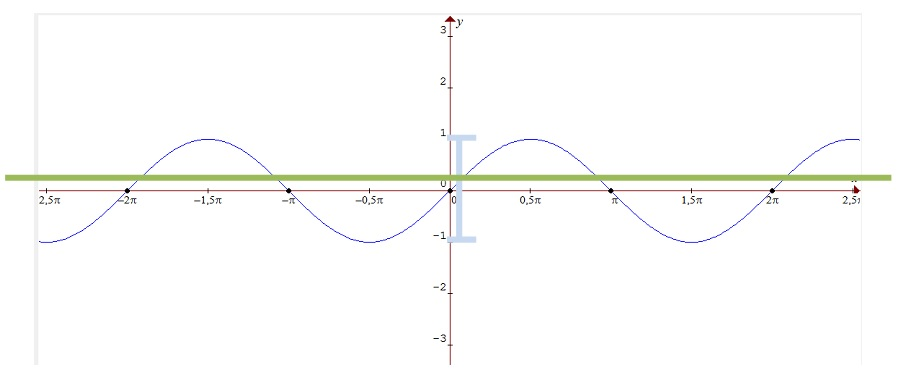
\includegraphics[height=5cm]{2_elem_rekenvaardigheden_B/inputs/reeel_vb3.jpg} 
%\end{figure}

%TODO figuur inladen
\begin{figure}
	\centering          
	
\begin{center}
\begin{tikzpicture}[scale=1,cap=round]

% Styles
\tikzstyle{axes}=[]
\tikzstyle help lines=[color=blue!50,very thin,dotted]


%%%%%%%%%%%%%%%%%%%%%%%%%%%%%%%%
%		GRID
%%%%%%%%%%%%%%%%%%%%%%%%%%%%%%%%

\draw[style=help lines,step=1cm] (-3.9,-5.9) grid (3.9,5.9);



%%%%%%%%%%%%%%%%%%%%%%%%%%%%%%%%
%		ASSENSTELSEL
%%%%%%%%%%%%%%%%%%%%%%%%%%%%%%%%

\draw[->] (-5,0) -- (7,0) node[right] {$x$};
\draw[->] (0,-7) -- (0,7) node[left]{$y$};

%\draw[fill,cyan](1,1)circle [radius=0.025];

%\draw[red,cap=rect, loosely dashed, ultra thick, domain=-2:2] plot (\x, {(\x*\x-1)+0.05}) node[above,yshift=-.7cm, right]{};

%%%%%%%%%%%%%%%%%%%%%%%%%%%%%%%%
%legende
%%%%%%%%%%%%%%%%%%%%%%%%%%%%%%%%
%\tkzDefPoint(0.5,3.5){A}
%\tkzDefPoint(1,3.5){B}
%\tkzLabelPoint[right,xshift=+0.1cm](B){${\color{cyan}f(x)=|x^2-1|}$}
%\tkzDrawSegment[cyan,ultra thick](A,B)

%\tkzDefPoint(0.5,3.2){C}
%\tkzDefPoint(1,3.2){D}
%\tkzLabelPoint[right,xshift=+0.1cm](D){${\color{red}e(x)=x^2-1}$}
%\tkzDrawSegment[red,cap=rect, loosely dashed, ultra thick](C,D)


%%%%%%%%%%%%%%%%%%%%%%%%%%%%%%%%
%getallen op de x-as en lijntjes
%%%%%%%%%%%%%%%%%%%%%%%%%%%%%%%%   
\foreach \x/\xtext in {-4,-3,-2,-1,1,2,3,4}
	\draw[xshift=\x cm] (0pt,1pt) -- (0pt,0pt) node[below,fill=white]
	{$\xtext$};,3
	
%getallen op de y-as en lijntjes  
%BEGIN LUS
\foreach \y/\ytext in {-6,-5,-4,-3,-2,-1,1,2,3,4,5,6}
	\draw[yshift=\y cm] (1pt,0pt) -- (0pt,0pt) node[left,fill=white]
	{$\ytext$}; %EINDE LUS



%%%%%%%%%%%%%%%%%%%%%%%%%%%%%%%%
%		GRAFIEKEN
%%%%%%%%%%%%%%%%%%%%%%%%%%%%%%%%
%\draw[cyan,cap=rect,thick, domain=-6:6] plot (\x, \x) node[above, right]{${\color{cyan}y=x}$};

\draw[cyan,cap=rect,ultra thick, domain=-1.2:3.5] plot (\x, {
	pow(\x,3)-3*pow(\x,2)		% <- plaats het functievoorschrift hier
}) node[above]{$f(x)=x^3-3x^2$};

 
%node[blue]{stijgen} 
%\draw[cyan,cap=rect,ultra thick, domain=2.25:6] plot (\x, {(\x-2)^(-1)}) node[above,yshift=+0.5cm,left]{$\color{cyan} y=\frac{1}{x-2}$};


%\draw[cyan,cap=rect,ultra thick, domain=-7:1.9] plot (\x, {exp{\x}}) node[above, right]{${\color{cyan}y=\exp{x}}$};

%%%%%%%%%%%%%%%%%%%%%%%%%%%%%%%%
%		MARKERINGEN
%%%%%%%%%%%%%%%%%%%%%%%%%%%%%%%%
%verticale lijn
%\draw[-o,line width=4,teal, cap=rect,opacity=0.3] (0,-4) -- (0,0.25) node[right] {};
%\draw[line width=4,teal, cap=rect,opacity=0.3] (0,0) -- (0,4.2) node[right] {bld $f$ = $\mathbb{R}_0$};
%horizontale lijn

 \draw[white,fill=blue,opacity=.5] (1,-2) circle [radius=.1]   node[blue, above,xshift=-1.1cm,opacity=1] {buigpunt in $(1,-2)$};


 
\draw[teal,cap=rect,line width=4, opacity=.5, domain=.5:1.5] plot (\x, {
	-2-3*(\x-1)		% <- plaats het functievoorschrift hier
}) node[opacity=1,above]{};


\draw[] (1.5,1.5) node[blue] {hol of concaaf};
\draw[] (1.5,-5) node[blue] {bol of convex};

\end{tikzpicture}
\end{center}

	\caption{voorbeeld 3}
	\label{fig:reele_functies_vb3}	
\end{figure}


\textbf{Domein}: we mogen op de plaats van $x$ gelijk welke
hoek invullen, de sinus zal steeds bestaan.

Besluit: $\textrm{dom}\:y=\mathbb{R}$ 




\textbf{Beeld}: we lezen op de $y$-as het beeld af. De
functiewaarden voor de sinus kunnen nooit groter zijn dan $1$ of
kleiner dan $-1$

Besluit: $\textrm{bld}f=[-1,1]$




\textbf{Nulpunten}: de $x$-as wordt gesneden als $\sin(x)=0$.
Dit gebeurt zowel voor $x$-waarden gelijk aan $\{0,\pi,2\pi,3\pi,...\}$
als ook voor $\{...,-3\pi,-2\pi,-\pi,0\}$

Besluit: de snijpunten met de $x$-as zijn de punten $\{...,(-2\pi,0),(-\pi,0),(0,0),(\pi,0),(2\pi,0),...\}$
of iets korter genoteerd als: $\{(k\pi,0)\:\textrm{met}\:k\in\mathbb{Z}\}$




\textbf{Symmetrie}: via de goniometrische formules vinden
we snel dat $f(-x)=\sin(-x)=-\sin(x)=-f(x)$ , dus kunnen we zeggen
dat deze functie oneven is (symmetrisch t.o.v. de oorsprong).

\end{voorbeeld}
%\subsection{Verloop van functies}

\subsubsection{Absolute en relatieve extrema}


\begin{definitie}
	Een functie $f$ heeft een \textbf{absoluut maximum} $f(x_{0})$
in het punt $x_{0}\in\textrm{dom}\:f$, als voor alle $x\in\textrm{dom}\:f$
geldt dat $f(x_{0})\geqslant f(x)$

Een functie $f$ heeft een \textbf{absoluut minimum} $f(x_{0})$
in het punt $x_{0}\in\textrm{dom}\:f$, als voor alle $x\in\textrm{dom}\:f$
geldt dat $f(x_{0})\leqslant f(x)$

Een functie $f$ heeft een \textbf{relatief of lokaal maximum}
in het punt $x_{0}$, indien er een open interval $I$ bestaat rond
het punt $x_{0}$ zodat voor alle $x$ in het interval $I$ geldt
dat $f(x_{0})\geqslant f(x)$

Een functie $f$ heeft een \textbf{relatief of lokaal minimum}
in het punt $x_{0}$, indien er een open interval $I$ bestaat rond
het punt $x_{0}$ zodat voor alle $x$ in het interval $I$ geldt
dat $f(x_{0})\leqslant f(x)$

\end{definitie}


\begin{voorbeeld}
%TODO figuur aanpassen  	

\begin{figure}[h]
	\centering          
	\begin{tikzpicture}[xscale=1,yscale=4,cap=round]

% Styles
\tikzstyle{axes}=[]
\tikzstyle help lines=[color=blue!50,very thin,dotted]

%%%%%%%%%%%%%%%%%%%%%%%%%%%%%%%%
%		GRID
%%%%%%%%%%%%%%%%%%%%%%%%%%%%%%%%

\draw[style=help lines,step=0.5cm] (-2.9,-0.6) grid (2.9,1.2);

%%%%%%%%%%%%%%%%%%%%%%%%%%%%%%%%
%		ASSENSTELSEL
%%%%%%%%%%%%%%%%%%%%%%%%%%%%%%%%

\draw[->] (-3,0) -- (3,0) node[right] {$x$};
\draw[->] (0,-0.6) -- (0,1.2) node[left]{$y$};

%\draw[fill,cyan](1,1)circle [radius=0.025];
%\draw[red,cap=rect, loosely dashed, ultra thick, domain=-2:2] plot (\x, {(\x*\x-1)+0.05}) node[above,yshift=-.7cm, right]{};

%%%%%%%%%%%%%%%%%%%%%%%%%%%%%%%%
%legende
%%%%%%%%%%%%%%%%%%%%%%%%%%%%%%%%
%\tkzDefPoint(0.5,3.5){A}
%\tkzDefPoint(1,3.5){B}
%\tkzLabelPoint[right,xshift=+0.1cm](B){${\color{cyan}f(x)=|x^2-1|}$}
%\tkzDrawSegment[cyan,ultra thick](A,B)

%\tkzDefPoint(0.5,3.2){C}
%\tkzDefPoint(1,3.2){D}
%\tkzLabelPoint[right,xshift=+0.1cm](D){${\color{red}e(x)=x^2-1}$}
%\tkzDrawSegment[red,cap=rect, loosely dashed, ultra thick](C,D)


%%%%%%%%%%%%%%%%%%%%%%%%%%%%%%%%
%getallen op de x-as en lijntjes
%%%%%%%%%%%%%%%%%%%%%%%%%%%%%%%%   
%\foreach \x/\xtext in {-2,-1,1,2}
%	\draw[xshift=\x cm] (0pt,1pt) -- (0pt,0pt) node[below,fill=white]
%	{$\xtext$};,3
	
%getallen op de y-as en lijntjes  
%BEGIN LUS
%\foreach \y/\ytext in {-1,1}
%	\draw[yshift=\y cm] (1pt,0pt) -- (0pt,0pt) node[left,fill=white]
%	{$\ytext$}; %EINDE LUS



%%%%%%%%%%%%%%%%%%%%%%%%%%%%%%%%
%		GRAFIEKEN
%%%%%%%%%%%%%%%%%%%%%%%%%%%%%%%%
%1.926583164702752926
%0.6148052613028164304
%%-14.35341068538563647
%-59.14215224350418509
%104.9541745028843565
%191

\draw[cyan,cap=rect,ultra thick, domain=-1.3:2.2] plot (\x, {
0.2*pow(\x,5)-(3/8)*pow(\x,4)-(2/3)*pow(\x,3)+(3/4)*pow(\x,2)+\x 	
%	*(	(\x+2)*(\x+1)*(\x+0.5)*(\x-1)*(\x-2) ) *0.2
	%pow(\x,5)+0.5*pow(\x,4)-5*pow(\x,3)+3*pow(\x,1)-1 )*.1 
	% <- plaats het functievoorschrift hier
}) node[above, yshift=+0.5cm,xshift=+1.3cm]{$$};
%f(x)=x^5+\frac{1}{2}x^4-5x^3-\frac{5}{2}x^2+4x-2

 
%node[blue]{stijgen} 
%\draw[cyan,cap=rect,ultra thick, domain=2.25:6] plot (\x, {(\x-2)^(-1)}) node[above,yshift=+0.5cm,left]{$\color{cyan} y=\frac{1}{x-2}$};


%\draw[cyan,cap=rect,ultra thick, domain=-7:1.9] plot (\x, {exp{\x}}) node[above, right]{${\color{cyan}y=\exp{x}}$};

%%%%%%%%%%%%%%%%%%%%%%%%%%%%%%%%
%		MARKERINGEN
%%%%%%%%%%%%%%%%%%%%%%%%%%%%%%%%
%verticale lijn
\draw[line width=1,red, dotted, opacity=1] (-1,-.15) -- (-1,0) node[above] {$x_1$};
\draw[line width=1,red, dotted, opacity=1] (-0.5,-.26) -- (-0.5,0) node[above] {$x_2$};
\draw[line width=1,red,opacity=1,dotted] (1,0) -- (1,0.9) node[above] {$x_3$};
\draw[line width=1,red,opacity=1,dotted] (2,0) -- (2,0.1) node[below,yshift=-.5cm] {$x_4$};
%\draw[line width=4,teal, cap=rect,opacity=0.3] (0,0) -- (0,4.2) node[right] {bld $f$ = $\mathbb{R}_0$};
%horizontale lijn

% \draw[white,fill=blue,opacity=.5] (1,-2) circle [radius=.1]   node[blue, above,xshift=-1.1cm,opacity=1] {buigpunt in $(1,-2)$};


 
%\draw[teal,cap=rect,line width=4, opacity=.5, domain=.5:1.5] plot (\x, {
%	-2-3*(\x-1)		% <- plaats het functievoorschrift hier
%}) node[opacity=1,above]{};


%\draw[] (1.5,1.5) node[blue] {hol of concaaf};
%\draw[] (1.5,-5) node[blue] {bol of convex};

\end{tikzpicture}
 
	\caption{voorbeeld 1}
	\label{fig:verloop_vb1}	
\end{figure}


Voor de functie in gegeven in bovenstaande figuur zijn $x_{1},\:x_{2},\:x_{3},\:x_{4}$ relatieve of lokale extrema. Hiervan zijn $x_{2}$ en $x_{3}$ absolute extrema.

$x_{1},\:x_{3}$ zijn relatieve of lokale maxima.
Hiervan is $x_{3}$ een absoluut maximum.

$x_{2},\:x_{4}$ zijn relatieve of lokale minima. Hiervan
is $x_{2}$ een absoluut minimum.

\end{voorbeeld}

\subsubsection{Stijgen, dalen en extrema}

De eerste afgeleide speelt een belangrijke rol bij het onderzoek
naar het verloop van een functie. Men zal dus het tekenverloop van
deze afgeleide onderzoeken.




\begin{definitie}
	Als de eerste afgeleide $f^{'}(x)>0$ is in een interval,
dan zal deze functie in dat interval \textbf{stijgen}.

Als de eerste afgeleide $f^{'}(x)<0$ is in een interval,
dan zal deze functie in dat interval \textbf{dalen}.

De functie zal een relatief of lokaal extremum (maximum
of minimum) bereiken waar de kromme overgaat van een stijgende functie
naar een dalende functie of omgekeerd.

Een functie $f(x)$ heeft in het punt $(x_{0},y_{0})$ een
extremum als in dat punt aan de volgende voorwaarden voldaan is:

\begin{itemize}
\item als $f^{'}(x_{0})=0$ en $f^{''}(x_{0})>0$ zal het
extremum een minimum zijn, en
\item als $f^{'}(x_{0})=0$ en $f^{''}(x_{0})<0$ zal het
extremum een maximum zijn.
\end{itemize}

\end{definitie}

\begin{opmerking}
	\ \\
	\begin{itemize}
\item Opmerking 1: in een extremum bezit de functie een horizontale
raaklijn (aangezien $f^{'}(x_{0})=0$ is).
\item Opmerking 2: indien $f^{'}(x_{0})=0$ en ook $f^{''}(x_{0})=0$
werkt deze methode niet om na te gaan of er in $x_{0}$ een extremum
is. In dat geval gaan we naar de derde afgeleide kijken. Als $f^{'''}(x_{0})\neq0$
dan is het punt $x_{0}$ een buigpunt. Indien ook de derde afgeleide
nul is moeten we naar de eerstvolgende afgeleide gaan kijken die niet
nul is. Stel dat deze van de n$^{de}$ orde is, dus $f^{(n)}(x_{0})\neq0$
. Als dan $n$ even is, is er in $x_{0}$ een lokaal minimum als $f^{(n)}(x_{0})>0$
, en een lokaal maximum als $f^{(n)}(x_{0})<0$ . Is de n$^{de}$
oneven dan is $x_{0}$ terug een buigpunt. 

Tip: als je dit moeilijk
kan onthouden, denk dan aan de eenvoudige functies $f(x)=x^{2}$ en
$f(x)=x^{3}$ . De functie $x^{2}$ heeft een minimum in nul, terwijl
$x^{3}$ in de oorsprong een buigpunt heeft.
\end{itemize}

\end{opmerking}



\begin{voorbeeld}
	Onderzoek het stijgen en dalen van volgende functie $f$ met voorschrift: $f(x)=x^{3}-3x^{2}$ in onderstaande figuur.
	
	\gewonefiguur{width=.7\linewidth}{2_elem_rekenvaardigheden_B/inputs/verloop_vb2.jpg}

De eerste afgeleide $f^{'}(x)=3x^{2}-6x$ is nul als $3x^{2}-6x=3x(x-2)=0$, dus als $x=0$ of als $x=2$.

Om de $y$-co\"ordinaat van deze extrema punten te vinden
vullen we $x=0$ en $x=2$ in in de functie $f(x)$. Dit geeft: $f(0)=0$
en $f(2)=-4$.

De functie $f$ zal in de punten $(0,0)$ en $(2,-4)$ een
extremum bezitten. In het punt $(0,0)$ is dit een maximum en in het
punt $(2,-4)$ een minimum. De raaklijn is in die punten ook telkens
horizontaal.

Aangezien de eerste afgeleide een tweedegraadsfunctie is,
zullen we het tekenverloop van de tweedegraadsfunctie toepassen, zie onderstaande tabel.

%\begin{table}
%	\centering
\begin{center}
	\begin{tabular}{c||c|c|c|c|c}
	$x$ &  & 0 &  & 2 & \tabularnewline
	\hline 
	$f^{'}(x)=3x(x-2)$ & + & 0 & - & 0 & + \\
	\hline 
	$f(x)$ &  & 0 &  & -4 & \\
	& $\nearrow$ & max & $\searrow$ & min & $\nearrow$ \\
\end{tabular}
\end{center}

%\caption{Voorbeeld stijgen, dalen en extrema.}
%\label{tab:stijgen}
%\end{table}

%\begin{figure}[h]
%\centering{}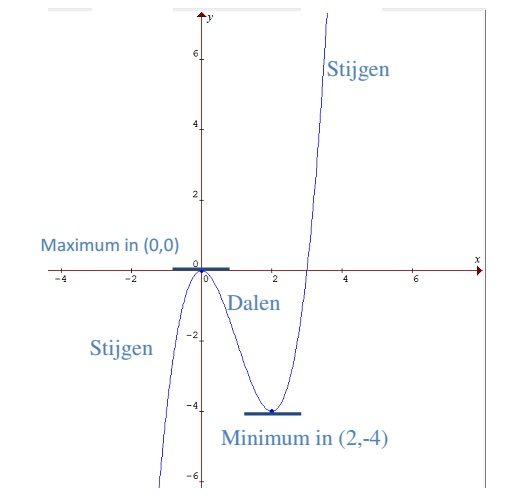
\includegraphics[width=.7\linewidth]{2_elem_rekenvaardigheden_B/inputs/verloop_vb2.jpg}
%\caption{Voorbeeld stijgen en dalen.}
%\label{fig:vb2}
%\end{figure}

\end{voorbeeld}

\subsubsection{Convex, concaaf en buigpunten}

Ook de tweede afgeleide speelt een belangrijke rol bij het
onderzoek naar het verloop van een functie. Men zal dus ook het tekenverloop
van de tweede afgeleide onderzoeken.


\begin{definitie}
	Als de tweede afgeleide $f^{''}(x)>0$ is in een interval,
dan zal de functie in dat interval \textbf{hol of concaaf} zijn (symbool:
$\bigcup$).

Als de tweede afgeleide $f^{''}(x)<0$ is in een interval,
dan zal de functie in dat interval \textbf{bol of convex} zijn (symbool:
$\bigcap$).

Punten waar de kromme overgaat van convex naar concaaf of
omgekeerd, noemt men \textbf{buigpunten}. In een buigpunt verandert
dus de tweede afgeleide van teken. Een functie $f(x)$ heeft in het
punt $(x_{0},y_{0})$ een buigpunt als in dat punt aan de volgende
voorwaarden voldaan zijn: $f^{''}(x_{0})=0$ en $f^{'''}(x_{0})\neq0$

\end{definitie}


\begin{opmerking}
	\ \\
	\begin{itemize}
	\item Opmerking 1: in een buigpunt snijdt de raaklijn de kromme,
	deze raaklijn noemt men de buigraaklijn.
	
	\item Opmerking 2: aangezien de kromming in een buigpunt verandert,
	is een buigpunt nooit een extremum.
\end{itemize}

\end{opmerking}


\begin{voorbeeld}
	Onderzoek het hol en bol zijn van
de functie $f$ met voorschrift $f(x)=x^{3}-3x^{2}$, zie onderstaande figuur.

\gewonefiguur{width=.7\linewidth}{2_elem_rekenvaardigheden_B/inputs/verloop_vb3.jpg}

De eerste afgeleide is $f^{'}(x)=3x^{2}-6x$ 

De tweede afgeleide is $f^{''}(x)=6x-6$ en is nul als $6x-6=6(x-1)=0$
, en dus als $x=1$.

Om de $y$-co\"ordinaat van dit buigpunt te vinden vullen
we $x=1$ in in de functie $f(x)$. Dit geeft: $f(1)=-2$.

Aangezien de tweede afgeleide een eerstegraadsfunctie is,
zullen we het tekenverloop van de eerstegraadsfunctie toepassen, zie onderstaande tabel.

%\begin{table}
%	\centering
\begin{center}
	\begin{tabular}{c||c|c|c}
	$x$ &  & 1 & \tabularnewline
	\hline 
	$f^{''}(x)=6(x-1)$ & - & 0 & +\\
	\hline 
	$f(x)$ & $\bigcap$ & -2 & $\bigcup$\\
	&  & buigpunt & \\
\end{tabular}
\end{center}
%\caption{Voorbeeld convex, concaaf en buigpunten}
%\label{tab:convex}
%\end{table}

\end{voorbeeld}
\begin{voorbeeld}
	Wat kan je zeggen over de functie $f$ met voorschrift
$f(x)=x^{3}$ in het punt waar $x=0$ is?

De eerste afgeleide is $f^{'}(x)=3x^{2}$ en is nul als
$x=0$. Dus $x=0$ kan een extremum zijn.

De tweede afgeleide is $f^{''}(x)=6x$ en is nul als $x=0$.
We kunnen niks zeggen; we moeten naar de eerstvolgende afgeleide gaan
kijken die niet nul is.

De derde afgeleide is $f^{'''}(x)=6$. De derde orde afgeleide
(n=3 is oneven) is niet nul, dus het punt $x=0$ is een buigpunt (en
geen extremum).

\end{voorbeeld}

\begin{voorbeeld}
	Zoek de buigpunten van de functie $f$ met voorschrift
$f(x)=\cos(x)$.

De eerste afgeleide is $f^{'}(x)=-\sin(x)$. De nulpunten
van $\sin x$ zijn $\{x=n\pi\:\textrm{met}\:n\in\mathbb{Z}\}$. In
deze punten kan $f(x)=\cos(x)$ een extremum bereiken.

De tweede afgeleide is $f^{''}(x)=-\cos(x)$. De nulpunten
van $\cos(x)$ zijn $\{x=\frac{\pi}{2}+n\pi\:\textrm{met}\:n\in\mathbb{Z}\}$.
In deze punten verandert de cosinus en dus ook de tweede afgeleide
van teken, dus dit zijn buigpunten. M.a.w. de nulpunten van de functie
$f(x)=\cos(x)$ zijn tevens de buigpunten (dit geldt ook voor de sinus).

\end{voorbeeld}
\subsection{Eerste- en tweedegraadsfuncties}
\label{sec:eerste_tweede}

\subsubsection{Constante functies}

\begin{definitie}
	Functievoorschrift: $f(x)=a$ met $a\in\mathbb{R}$
\end{definitie}

%\uline{Voorbeeld}: $f(x)=2$

\textbf{Grafische voorstelling van de constante functie}
met vergelijking $f(x)=a$ is een horizontale rechte, waarbij de $y$-as
wordt gesneden in het punt $(0,a)$.

%Alle afgeleiden zijn overal nul, er zijn geen extrema, geen
%buigpunten...

Tekenverloop: 

\begin{tabel}{Tekenverloop van een constante functie}
	\begin{tabular}{c||c}
		$x$ & \\
		\hline 
		$f(x)$ & teken van $a$\\
	\end{tabular}
	\label{tab:ct}
\end{tabel}


\begin{voorbeeld}
	Gegeven de functie: $f(x)=\frac{1}{2}$. 
%TODO figuur

\begin{figure}[h]
	\centering          
	\tikzsetfigurename{Fig_module_2_1_4_constante_functie}
\begin{tikzpicture}

% Styles
\tikzstyle{axes}=[]
\tikzstyle help lines=[color=blue!50,very thin,dotted]


%%%%%%%%%%%%%%%%%%%%%%%%%%%%%%%%
%		GRID
%%%%%%%%%%%%%%%%%%%%%%%%%%%%%%%%

\draw[style=help lines,step=1cm] (-3.9,-2.9) grid (3.9,2.9);



%%%%%%%%%%%%%%%%%%%%%%%%%%%%%%%%
%		ASSENSTELSEL
%%%%%%%%%%%%%%%%%%%%%%%%%%%%%%%%

\draw[->] (-5,0) -- (5,0) node[right] {$x$};
\draw[->] (0,-3) -- (0,3) node[left]{$y$};

%\draw[fill,cyan](1,1)circle [radius=0.025];

%\draw[red,cap=rect, loosely dashed, ultra thick, domain=-2:2] plot (\x, {(\x*\x-1)+0.05}) node[above,yshift=-.7cm, right]{};

%%%%%%%%%%%%%%%%%%%%%%%%%%%%%%%%
%legende
%%%%%%%%%%%%%%%%%%%%%%%%%%%%%%%%
%\tkzDefPoint(0.5,3.5){A}
%\tkzDefPoint(1,3.5){B}
%\tkzLabelPoint[right,xshift=+0.1cm](B){${\color{cyan}f(x)=|x^2-1|}$}
%\tkzDrawSegment[cyan,ultra thick](A,B)

%\tkzDefPoint(0.5,3.2){C}
%\tkzDefPoint(1,3.2){D}
%\tkzLabelPoint[right,xshift=+0.1cm](D){${\color{red}e(x)=x^2-1}$}
%\tkzDrawSegment[red,cap=rect, loosely dashed, ultra thick](C,D)


%%%%%%%%%%%%%%%%%%%%%%%%%%%%%%%%
%getallen op de x-as en lijntjes
%%%%%%%%%%%%%%%%%%%%%%%%%%%%%%%%   
\foreach \x/\xtext in {-4,-3,-2,-1,0,1,2,3,4}
	\draw[xshift=\x cm] (0pt,1pt) -- (0pt,0pt) node[below,fill=white]
	{$\xtext$};,3
	
%getallen op de y-as en lijntjes  
%BEGIN LUS
\foreach \y/\ytext in {-2,-1,1,2}
	\draw[yshift=\y cm] (1pt,0pt) -- (0pt,0pt) node[left,fill=white]
	{$\ytext$}; %EINDE LUS



%%%%%%%%%%%%%%%%%%%%%%%%%%%%%%%%
%		GRAFIEKEN
%%%%%%%%%%%%%%%%%%%%%%%%%%%%%%%%
%\draw[cyan,cap=rect,thick, domain=-6:6] plot (\x, \x) node[above, right]{${\color{cyan}y=x}$};


\draw[teal,cap=rect,line width=4, opacity=.5, domain=-5:5] plot (\x, {
	0.5		% <- plaats het functievoorschrift hier
}) node[opacity=1,above]{};


 
%node[blue]{stijgen} 
%\draw[cyan,cap=rect,ultra thick, domain=2.25:6] plot (\x, {(\x-2)^(-1)}) node[above,yshift=+0.5cm,left]{$\color{cyan} y=\frac{1}{x-2}$};


%\draw[cyan,cap=rect,ultra thick, domain=-7:1.9] plot (\x, {exp{\x}}) node[above, right]{${\color{cyan}y=\exp{x}}$};

%%%%%%%%%%%%%%%%%%%%%%%%%%%%%%%%
%		MARKERINGEN
%%%%%%%%%%%%%%%%%%%%%%%%%%%%%%%%
%verticale lijn
%\draw[-o,line width=4,teal, cap=rect,opacity=0.3] (0,-4) -- (0,0.25) node[right] {};
%\draw[line width=4,teal, cap=rect,opacity=0.3] (0,0) -- (0,4.2) node[right] {bld $f$ = $\mathbb{R}_0$};
%horizontale lijn

% \draw[white,fill=blue,opacity=.5] (1,-2) circle [radius=.1]   node[blue, above,xshift=-1.1cm,opacity=1] {buigpunt in $(1,-2)$};


 


\draw[] (0,.5) node[blue,left] {$\frac{1}{2}$};
%\draw[] (1.5,-5) node[blue] {bol of convex};

\end{tikzpicture}
 
	\caption{Voorbeeld constante functie}
	\label{fig:constante_functie}	
\end{figure}
	
 
Grafische voorstelling:
\begin{itemize}
\item het domein van de constante functie is altijd: $\textrm{dom}f=\mathbb{R}$
\item het beeld van deze constante functie is: $\textrm{bld}f=\frac{1}{2}$
\end{itemize}
%\begin{figure}[h]
%\centering{}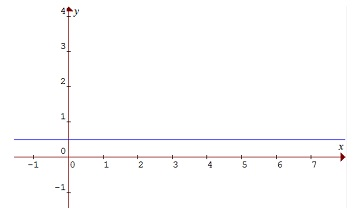
\includegraphics[height=5cm]{2_elem_rekenvaardigheden_B/inputs/constantefuncties.jpg} 
%\caption{Voorbeeld constante functie.}
%\label{fig:ct}
%\end{figure}

Tekenverloop

\begin{center}
\begin{tabular}{c||c}
	$x$ & \\
	\hline 
	$f(x)$ & $+$ \\
\end{tabular}	
\end{center}

\end{voorbeeld}

\subsubsection{Eerstegraadsfuncties of lineaire functies}

\begin{definitie}
	Functievoorschrift: $f(x)=ax+b$ met $a\in\mathbb{R}_{0}$
en $b\in\mathbb{R}$.

\end{definitie}


\begin{voorbeeld}
	 $f(x)=10x+1$ , $f(x)=8-5x$ , $f(x)=3x$
\end{voorbeeld}

Grafische voorstelling van de lineaire functie is een rechte.

%TODO figuur

\begin{figure}[h]
	\centering          
	\begin{tikzpicture}[scale=1,cap=round]

% Styles
\tikzstyle{axes}=[]
\tikzstyle help lines=[color=blue!50,very thin,dotted]


%%%%%%%%%%%%%%%%%%%%%%%%%%%%%%%%
%		GRID
%%%%%%%%%%%%%%%%%%%%%%%%%%%%%%%%

\draw[style=help lines,step=1cm] (-3.9,-2.9) grid (3.9,5.9);



%%%%%%%%%%%%%%%%%%%%%%%%%%%%%%%%
%		ASSENSTELSEL
%%%%%%%%%%%%%%%%%%%%%%%%%%%%%%%%

\draw[->] (-5,0) -- (5,0) node[right] {$x$};
\draw[->] (0,-4) -- (0,7) node[left]{$y$};

%\draw[fill,cyan](1,1)circle [radius=0.025];

%\draw[red,cap=rect, loosely dashed, ultra thick, domain=-2:2] plot (\x, {(\x*\x-1)+0.05}) node[above,yshift=-.7cm, right]{};

%%%%%%%%%%%%%%%%%%%%%%%%%%%%%%%%
%legende
%%%%%%%%%%%%%%%%%%%%%%%%%%%%%%%%
%\tkzDefPoint(0.5,3.5){A}
%\tkzDefPoint(1,3.5){B}
%\tkzLabelPoint[right,xshift=+0.1cm](B){${\color{cyan}f(x)=|x^2-1|}$}
%\tkzDrawSegment[cyan,ultra thick](A,B)

%\tkzDefPoint(0.5,3.2){C}
%\tkzDefPoint(1,3.2){D}
%\tkzLabelPoint[right,xshift=+0.1cm](D){${\color{red}e(x)=x^2-1}$}
%\tkzDrawSegment[red,cap=rect, loosely dashed, ultra thick](C,D)


%%%%%%%%%%%%%%%%%%%%%%%%%%%%%%%%
%getallen op de x-as en lijntjes
%%%%%%%%%%%%%%%%%%%%%%%%%%%%%%%%   
\foreach \x/\xtext in {-4,-3,-2,-1,0,1,2,3,4}
	\draw[xshift=\x cm] (0pt,1pt) -- (0pt,0pt) node[below,fill=white]
	{$\xtext$};,3
	
%getallen op de y-as en lijntjes  
%BEGIN LUS
\foreach \y/\ytext in {-3,-2,-1,1,2,3,4,5,6}
	\draw[yshift=\y cm] (1pt,0pt) -- (0pt,0pt) node[left,fill=white]
	{$\ytext$}; %EINDE LUS



%%%%%%%%%%%%%%%%%%%%%%%%%%%%%%%%
%		GRAFIEKEN
%%%%%%%%%%%%%%%%%%%%%%%%%%%%%%%%
%\draw[cyan,cap=rect,thick, domain=-6:6] plot (\x, \x) node[above, right]{${\color{cyan}y=x}$};


\draw[teal,cap=rect,line width=4, opacity=.5, domain=-3:2] plot (\x, {
	2*\x + 3 		% <- plaats het functievoorschrift hier
}) node[opacity=1,left,pos=1,xshift=-1cm, yshift=+2cm]{$q=3$};
 
%node[blue]{stijgen} 
%\draw[cyan,cap=rect,ultra thick, domain=2.25:6] plot (\x, {(\x-2)^(-1)}) node[above,yshift=+0.5cm,left]{$\color{cyan} y=\frac{1}{x-2}$};


%\draw[cyan,cap=rect,ultra thick, domain=-7:1.9] plot (\x, {exp{\x}}) node[above, right]{${\color{cyan}y=\exp{x}}$};

%%%%%%%%%%%%%%%%%%%%%%%%%%%%%%%%
%		MARKERINGEN
%%%%%%%%%%%%%%%%%%%%%%%%%%%%%%%%
%verticale lijn
%\draw[-o,line width=4,teal, cap=rect,opacity=0.3] (0,-4) -- (0,0.25) node[right] {};
%\draw[line width=4,teal, cap=rect,opacity=0.3] (0,0) -- (0,4.2) node[right] {bld $f$ = $\mathbb{R}_0$};
%horizontale lijn

%horizontale lijn
\draw[->,line width=1,red, cap=rect,opacity=1] (0,3) -- (1,3) node[right] {$1$};
\draw[->,line width=1,red, cap=rect,opacity=1] (1,3) -- (1,5) node[right,pos=0.5] {$m=2$};



% \draw[white,fill=blue,opacity=.5] (1,-2) circle [radius=.1]   node[blue, above,xshift=-1.1cm,opacity=1] {buigpunt in $(1,-2)$};

\draw[] (2,2) node[blue,right] {$y=mx +q$};

\draw[] (2,1) node[blue,right] {$y=2x +3$};

\end{tikzpicture}
 
	\caption{Voorbeeld van een eerstegraadsfunctie}
	\label{fig:eerstegraadsfunctie}	
\end{figure}



%\gewonefiguur{height=5cm}{2_elem_rekenvaardigheden_B/inputs/eerstegraadsfuncties1.jpg}

\begin{itemize}
	\item Het domein van elke lineaire functie is: $\textrm{dom} f = \mathbb{R}$.
	\item Het beeld van deze lineaire functie is: $\textrm{bld} f = \mathbb{R}$.
\end{itemize}

De rechte wordt bepaald door de \textbf{richtingsco\"effici\"ent}
(de \textbf{rico}) \textquoteleft $a$\textquoteright{} en de intercept
\textquoteleft $b$\textquoteright . De rico bepaalt de helling van
de rechte. Als $x$ met 1 eenheid toeneemt, dan neemt $y$ met $a$
eenheden toe. Hoe groter de absolute waarde van de rico $a$, hoe
steiler de rechte.
\begin{itemize}
\item een positieve rico hoort bij een stijgende rechte
\item een negatieve rico hoort bij een dalende rechte
\end{itemize}


%TODO figuur

%M\begin{tabular}{ccc}
	%\hline
%	\begin{tikzpicture}[scale=0.3,cap=round]

% Styles
\tikzstyle{axes}=[]
\tikzstyle help lines=[color=blue!50,very thin,dotted]


%%%%%%%%%%%%%%%%%%%%%%%%%%%%%%%%
%		GRID
%%%%%%%%%%%%%%%%%%%%%%%%%%%%%%%%

\draw[style=help lines,step=1cm] (-3.9,-2.9) grid (3.9,5.9);



%%%%%%%%%%%%%%%%%%%%%%%%%%%%%%%%
%		ASSENSTELSEL
%%%%%%%%%%%%%%%%%%%%%%%%%%%%%%%%

\draw[->] (-5,0) -- (5,0) node[right] {$x$};
\draw[->] (0,-4) -- (0,7) node[left]{$y$};

%\draw[fill,cyan](1,1)circle [radius=0.025];

%\draw[red,cap=rect, loosely dashed, ultra thick, domain=-2:2] plot (\x, {(\x*\x-1)+0.05}) node[above,yshift=-.7cm, right]{};

%%%%%%%%%%%%%%%%%%%%%%%%%%%%%%%%
%legende
%%%%%%%%%%%%%%%%%%%%%%%%%%%%%%%%
%\tkzDefPoint(0.5,3.5){A}
%\tkzDefPoint(1,3.5){B}
%\tkzLabelPoint[right,xshift=+0.1cm](B){${\color{cyan}f(x)=|x^2-1|}$}
%\tkzDrawSegment[cyan,ultra thick](A,B)

%\tkzDefPoint(0.5,3.2){C}
%\tkzDefPoint(1,3.2){D}
%\tkzLabelPoint[right,xshift=+0.1cm](D){${\color{red}e(x)=x^2-1}$}
%\tkzDrawSegment[red,cap=rect, loosely dashed, ultra thick](C,D)


%%%%%%%%%%%%%%%%%%%%%%%%%%%%%%%%
%getallen op de x-as en lijntjes
%%%%%%%%%%%%%%%%%%%%%%%%%%%%%%%%   
\foreach \x/\xtext in {-4,-3,-2,-1,0,1,2,3,4}
	\draw[xshift=\x cm] (0pt,1pt) -- (0pt,0pt) node[below,fill=white]
	{$\xtext$};,3
	
%getallen op de y-as en lijntjes  
%BEGIN LUS
\foreach \y/\ytext in {-3,-2,-1,1,2,3,4,5,6}
	\draw[yshift=\y cm] (1pt,0pt) -- (0pt,0pt) node[left,fill=white]
	{$\ytext$}; %EINDE LUS



%%%%%%%%%%%%%%%%%%%%%%%%%%%%%%%%
%		GRAFIEKEN
%%%%%%%%%%%%%%%%%%%%%%%%%%%%%%%%
%\draw[cyan,cap=rect,thick, domain=-6:6] plot (\x, \x) node[above, right]{${\color{cyan}y=x}$};


\draw[teal,cap=rect,line width=4, opacity=.5, domain=-3:2] plot (\x, {
	2*\x + 3 		% <- plaats het functievoorschrift hier
}) node[opacity=1,left,pos=1,xshift=-1cm, yshift=+2cm]{$q=3$};
 
%node[blue]{stijgen} 
%\draw[cyan,cap=rect,ultra thick, domain=2.25:6] plot (\x, {(\x-2)^(-1)}) node[above,yshift=+0.5cm,left]{$\color{cyan} y=\frac{1}{x-2}$};


%\draw[cyan,cap=rect,ultra thick, domain=-7:1.9] plot (\x, {exp{\x}}) node[above, right]{${\color{cyan}y=\exp{x}}$};

%%%%%%%%%%%%%%%%%%%%%%%%%%%%%%%%
%		MARKERINGEN
%%%%%%%%%%%%%%%%%%%%%%%%%%%%%%%%
%verticale lijn
%\draw[-o,line width=4,teal, cap=rect,opacity=0.3] (0,-4) -- (0,0.25) node[right] {};
%\draw[line width=4,teal, cap=rect,opacity=0.3] (0,0) -- (0,4.2) node[right] {bld $f$ = $\mathbb{R}_0$};
%horizontale lijn

%horizontale lijn



% \draw[white,fill=blue,opacity=.5] (1,-2) circle [radius=.1]   node[blue, above,xshift=-1.1cm,opacity=1] {buigpunt in $(1,-2)$};

\draw[] (2,2) node[blue,right] {$ m > 0 $};



\end{tikzpicture}
 	&\tikzsetfigurename{Fig_module_2_1_4_rico_nul}

\begin{tikzpicture}[scale=0.3,cap=round]

% Styles
\tikzstyle{axes}=[]
\tikzstyle help lines=[color=blue!50,very thin,dotted]


%%%%%%%%%%%%%%%%%%%%%%%%%%%%%%%%
%		GRID
%%%%%%%%%%%%%%%%%%%%%%%%%%%%%%%%

\draw[style=help lines,step=1cm] (-3.9,-2.9) grid (3.9,5.9);



%%%%%%%%%%%%%%%%%%%%%%%%%%%%%%%%
%		ASSENSTELSEL
%%%%%%%%%%%%%%%%%%%%%%%%%%%%%%%%

\draw[->] (-5,0) -- (5,0) node[right] {$x$};
\draw[->] (0,-4) -- (0,7) node[left]{$y$};

%\draw[fill,cyan](1,1)circle [radius=0.025];

%\draw[red,cap=rect, loosely dashed, ultra thick, domain=-2:2] plot (\x, {(\x*\x-1)+0.05}) node[above,yshift=-.7cm, right]{};

%%%%%%%%%%%%%%%%%%%%%%%%%%%%%%%%
%legende
%%%%%%%%%%%%%%%%%%%%%%%%%%%%%%%%
%\tkzDefPoint(0.5,3.5){A}
%\tkzDefPoint(1,3.5){B}
%\tkzLabelPoint[right,xshift=+0.1cm](B){${\color{cyan}f(x)=|x^2-1|}$}
%\tkzDrawSegment[cyan,ultra thick](A,B)

%\tkzDefPoint(0.5,3.2){C}
%\tkzDefPoint(1,3.2){D}
%\tkzLabelPoint[right,xshift=+0.1cm](D){${\color{red}e(x)=x^2-1}$}
%\tkzDrawSegment[red,cap=rect, loosely dashed, ultra thick](C,D)


%%%%%%%%%%%%%%%%%%%%%%%%%%%%%%%%
%getallen op de x-as en lijntjes
%%%%%%%%%%%%%%%%%%%%%%%%%%%%%%%%   
\foreach \x/\xtext in {-4,-3,-2,-1,0,1,2,3,4}
	\draw[xshift=\x cm] (0pt,1pt) -- (0pt,0pt) node[below,fill=white]
	{$\xtext$};,3
	
%getallen op de y-as en lijntjes  
%BEGIN LUS
\foreach \y/\ytext in {-3,-2,-1,1,2,3,4,5,6}
	\draw[yshift=\y cm] (1pt,0pt) -- (0pt,0pt) node[left,fill=white]
	{$\ytext$}; %EINDE LUS



%%%%%%%%%%%%%%%%%%%%%%%%%%%%%%%%
%		GRAFIEKEN
%%%%%%%%%%%%%%%%%%%%%%%%%%%%%%%%
%\draw[cyan,cap=rect,thick, domain=-6:6] plot (\x, \x) node[above, right]{${\color{cyan}y=x}$};


\draw[teal,cap=rect,line width=4, opacity=.5, domain=-5:5] plot (\x, {
	2.3 		% <- plaats het functievoorschrift hier
}) node[opacity=1,left,pos=1,xshift=-1cm, yshift=+2cm]{$q=3$};
 
%node[blue]{stijgen} 
%\draw[cyan,cap=rect,ultra thick, domain=2.25:6] plot (\x, {(\x-2)^(-1)}) node[above,yshift=+0.5cm,left]{$\color{cyan} y=\frac{1}{x-2}$};


%\draw[cyan,cap=rect,ultra thick, domain=-7:1.9] plot (\x, {exp{\x}}) node[above, right]{${\color{cyan}y=\exp{x}}$};

%%%%%%%%%%%%%%%%%%%%%%%%%%%%%%%%
%		MARKERINGEN
%%%%%%%%%%%%%%%%%%%%%%%%%%%%%%%%
%verticale lijn
%\draw[-o,line width=4,teal, cap=rect,opacity=0.3] (0,-4) -- (0,0.25) node[right] {};
%\draw[line width=4,teal, cap=rect,opacity=0.3] (0,0) -- (0,4.2) node[right] {bld $f$ = $\mathbb{R}_0$};
%horizontale lijn

%horizontale lijn





% \draw[white,fill=blue,opacity=.5] (1,-2) circle [radius=.1]   node[blue, above,xshift=-1.1cm,opacity=1] {buigpunt in $(1,-2)$};

\draw[] (2,3) node[blue,right] {$m=0$};



\end{tikzpicture}
  &  \begin{tikzpicture}[scale=0.3,cap=round]

% Styles
\tikzstyle{axes}=[]
\tikzstyle help lines=[color=blue!50,very thin,dotted]


%%%%%%%%%%%%%%%%%%%%%%%%%%%%%%%%
%		GRID
%%%%%%%%%%%%%%%%%%%%%%%%%%%%%%%%

\draw[style=help lines,step=1cm] (-3.9,-2.9) grid (3.9,5.9);



%%%%%%%%%%%%%%%%%%%%%%%%%%%%%%%%
%		ASSENSTELSEL
%%%%%%%%%%%%%%%%%%%%%%%%%%%%%%%%

\draw[->] (-5,0) -- (5,0) node[right] {$x$};
\draw[->] (0,-4) -- (0,7) node[left]{$y$};

%\draw[fill,cyan](1,1)circle [radius=0.025];

%\draw[red,cap=rect, loosely dashed, ultra thick, domain=-2:2] plot (\x, {(\x*\x-1)+0.05}) node[above,yshift=-.7cm, right]{};

%%%%%%%%%%%%%%%%%%%%%%%%%%%%%%%%
%legende
%%%%%%%%%%%%%%%%%%%%%%%%%%%%%%%%
%\tkzDefPoint(0.5,3.5){A}
%\tkzDefPoint(1,3.5){B}
%\tkzLabelPoint[right,xshift=+0.1cm](B){${\color{cyan}f(x)=|x^2-1|}$}
%\tkzDrawSegment[cyan,ultra thick](A,B)

%\tkzDefPoint(0.5,3.2){C}
%\tkzDefPoint(1,3.2){D}
%\tkzLabelPoint[right,xshift=+0.1cm](D){${\color{red}e(x)=x^2-1}$}
%\tkzDrawSegment[red,cap=rect, loosely dashed, ultra thick](C,D)


%%%%%%%%%%%%%%%%%%%%%%%%%%%%%%%%
%getallen op de x-as en lijntjes
%%%%%%%%%%%%%%%%%%%%%%%%%%%%%%%%   
\foreach \x/\xtext in {-4,-3,-2,-1,0,1,2,3,4}
	\draw[xshift=\x cm] (0pt,1pt) -- (0pt,0pt) node[below,fill=white]
	{$\xtext$};,3
	
%getallen op de y-as en lijntjes  
%BEGIN LUS
\foreach \y/\ytext in {-3,-2,-1,1,2,3,4,5,6}
	\draw[yshift=\y cm] (1pt,0pt) -- (0pt,0pt) node[left,fill=white]
	{$\ytext$}; %EINDE LUS



%%%%%%%%%%%%%%%%%%%%%%%%%%%%%%%%
%		GRAFIEKEN
%%%%%%%%%%%%%%%%%%%%%%%%%%%%%%%%
%\draw[cyan,cap=rect,thick, domain=-6:6] plot (\x, \x) node[above, right]{${\color{cyan}y=x}$};


\draw[teal,cap=rect,line width=4, opacity=.5, domain=-1:3] plot (\x, {
	(-2)*\x + 3  		% <- plaats het functievoorschrift hier
}) node[opacity=1,left,pos=1,xshift=-1cm, yshift=+2cm]{$q=3$};
 
%node[blue]{stijgen} 
%\draw[cyan,cap=rect,ultra thick, domain=2.25:6] plot (\x, {(\x-2)^(-1)}) node[above,yshift=+0.5cm,left]{$\color{cyan} y=\frac{1}{x-2}$};


%\draw[cyan,cap=rect,ultra thick, domain=-7:1.9] plot (\x, {exp{\x}}) node[above, right]{${\color{cyan}y=\exp{x}}$};

%%%%%%%%%%%%%%%%%%%%%%%%%%%%%%%%
%		MARKERINGEN
%%%%%%%%%%%%%%%%%%%%%%%%%%%%%%%%
%verticale lijn
%\draw[-o,line width=4,teal, cap=rect,opacity=0.3] (0,-4) -- (0,0.25) node[right] {};
%\draw[line width=4,teal, cap=rect,opacity=0.3] (0,0) -- (0,4.2) node[right] {bld $f$ = $\mathbb{R}_0$};
%horizontale lijn

%horizontale lijn




% \draw[white,fill=blue,opacity=.5] (1,-2) circle [radius=.1]   node[blue, above,xshift=-1.1cm,opacity=1] {buigpunt in $(1,-2)$};

\draw[] (2,2) node[blue,right] {$m<0$};



\end{tikzpicture}
   \\
	%\hline
%\end{tabular}


\begin{figure}[h]
	\centering
	\begin{subfigure}{0.3\textwidth}
	\begin{tikzpicture}[scale=0.3,cap=round]

% Styles
\tikzstyle{axes}=[]
\tikzstyle help lines=[color=blue!50,very thin,dotted]


%%%%%%%%%%%%%%%%%%%%%%%%%%%%%%%%
%		GRID
%%%%%%%%%%%%%%%%%%%%%%%%%%%%%%%%

\draw[style=help lines,step=1cm] (-3.9,-2.9) grid (3.9,5.9);



%%%%%%%%%%%%%%%%%%%%%%%%%%%%%%%%
%		ASSENSTELSEL
%%%%%%%%%%%%%%%%%%%%%%%%%%%%%%%%

\draw[->] (-5,0) -- (5,0) node[right] {$x$};
\draw[->] (0,-4) -- (0,7) node[left]{$y$};

%\draw[fill,cyan](1,1)circle [radius=0.025];

%\draw[red,cap=rect, loosely dashed, ultra thick, domain=-2:2] plot (\x, {(\x*\x-1)+0.05}) node[above,yshift=-.7cm, right]{};

%%%%%%%%%%%%%%%%%%%%%%%%%%%%%%%%
%legende
%%%%%%%%%%%%%%%%%%%%%%%%%%%%%%%%
%\tkzDefPoint(0.5,3.5){A}
%\tkzDefPoint(1,3.5){B}
%\tkzLabelPoint[right,xshift=+0.1cm](B){${\color{cyan}f(x)=|x^2-1|}$}
%\tkzDrawSegment[cyan,ultra thick](A,B)

%\tkzDefPoint(0.5,3.2){C}
%\tkzDefPoint(1,3.2){D}
%\tkzLabelPoint[right,xshift=+0.1cm](D){${\color{red}e(x)=x^2-1}$}
%\tkzDrawSegment[red,cap=rect, loosely dashed, ultra thick](C,D)


%%%%%%%%%%%%%%%%%%%%%%%%%%%%%%%%
%getallen op de x-as en lijntjes
%%%%%%%%%%%%%%%%%%%%%%%%%%%%%%%%   
\foreach \x/\xtext in {-4,-3,-2,-1,0,1,2,3,4}
	\draw[xshift=\x cm] (0pt,1pt) -- (0pt,0pt) node[below,fill=white]
	{$\xtext$};,3
	
%getallen op de y-as en lijntjes  
%BEGIN LUS
\foreach \y/\ytext in {-3,-2,-1,1,2,3,4,5,6}
	\draw[yshift=\y cm] (1pt,0pt) -- (0pt,0pt) node[left,fill=white]
	{$\ytext$}; %EINDE LUS



%%%%%%%%%%%%%%%%%%%%%%%%%%%%%%%%
%		GRAFIEKEN
%%%%%%%%%%%%%%%%%%%%%%%%%%%%%%%%
%\draw[cyan,cap=rect,thick, domain=-6:6] plot (\x, \x) node[above, right]{${\color{cyan}y=x}$};


\draw[teal,cap=rect,line width=4, opacity=.5, domain=-3:2] plot (\x, {
	2*\x + 3 		% <- plaats het functievoorschrift hier
}) node[opacity=1,left,pos=1,xshift=-1cm, yshift=+2cm]{$q=3$};
 
%node[blue]{stijgen} 
%\draw[cyan,cap=rect,ultra thick, domain=2.25:6] plot (\x, {(\x-2)^(-1)}) node[above,yshift=+0.5cm,left]{$\color{cyan} y=\frac{1}{x-2}$};


%\draw[cyan,cap=rect,ultra thick, domain=-7:1.9] plot (\x, {exp{\x}}) node[above, right]{${\color{cyan}y=\exp{x}}$};

%%%%%%%%%%%%%%%%%%%%%%%%%%%%%%%%
%		MARKERINGEN
%%%%%%%%%%%%%%%%%%%%%%%%%%%%%%%%
%verticale lijn
%\draw[-o,line width=4,teal, cap=rect,opacity=0.3] (0,-4) -- (0,0.25) node[right] {};
%\draw[line width=4,teal, cap=rect,opacity=0.3] (0,0) -- (0,4.2) node[right] {bld $f$ = $\mathbb{R}_0$};
%horizontale lijn

%horizontale lijn



% \draw[white,fill=blue,opacity=.5] (1,-2) circle [radius=.1]   node[blue, above,xshift=-1.1cm,opacity=1] {buigpunt in $(1,-2)$};

\draw[] (2,2) node[blue,right] {$ m > 0 $};



\end{tikzpicture}
 
	\caption{}
	\label{fig:rico_pos}	
	\end{subfigure}
	\begin{subfigure}{0.3\textwidth}
	\tikzsetfigurename{Fig_module_2_1_4_rico_nul}

\begin{tikzpicture}[scale=0.3,cap=round]

% Styles
\tikzstyle{axes}=[]
\tikzstyle help lines=[color=blue!50,very thin,dotted]


%%%%%%%%%%%%%%%%%%%%%%%%%%%%%%%%
%		GRID
%%%%%%%%%%%%%%%%%%%%%%%%%%%%%%%%

\draw[style=help lines,step=1cm] (-3.9,-2.9) grid (3.9,5.9);



%%%%%%%%%%%%%%%%%%%%%%%%%%%%%%%%
%		ASSENSTELSEL
%%%%%%%%%%%%%%%%%%%%%%%%%%%%%%%%

\draw[->] (-5,0) -- (5,0) node[right] {$x$};
\draw[->] (0,-4) -- (0,7) node[left]{$y$};

%\draw[fill,cyan](1,1)circle [radius=0.025];

%\draw[red,cap=rect, loosely dashed, ultra thick, domain=-2:2] plot (\x, {(\x*\x-1)+0.05}) node[above,yshift=-.7cm, right]{};

%%%%%%%%%%%%%%%%%%%%%%%%%%%%%%%%
%legende
%%%%%%%%%%%%%%%%%%%%%%%%%%%%%%%%
%\tkzDefPoint(0.5,3.5){A}
%\tkzDefPoint(1,3.5){B}
%\tkzLabelPoint[right,xshift=+0.1cm](B){${\color{cyan}f(x)=|x^2-1|}$}
%\tkzDrawSegment[cyan,ultra thick](A,B)

%\tkzDefPoint(0.5,3.2){C}
%\tkzDefPoint(1,3.2){D}
%\tkzLabelPoint[right,xshift=+0.1cm](D){${\color{red}e(x)=x^2-1}$}
%\tkzDrawSegment[red,cap=rect, loosely dashed, ultra thick](C,D)


%%%%%%%%%%%%%%%%%%%%%%%%%%%%%%%%
%getallen op de x-as en lijntjes
%%%%%%%%%%%%%%%%%%%%%%%%%%%%%%%%   
\foreach \x/\xtext in {-4,-3,-2,-1,0,1,2,3,4}
	\draw[xshift=\x cm] (0pt,1pt) -- (0pt,0pt) node[below,fill=white]
	{$\xtext$};,3
	
%getallen op de y-as en lijntjes  
%BEGIN LUS
\foreach \y/\ytext in {-3,-2,-1,1,2,3,4,5,6}
	\draw[yshift=\y cm] (1pt,0pt) -- (0pt,0pt) node[left,fill=white]
	{$\ytext$}; %EINDE LUS



%%%%%%%%%%%%%%%%%%%%%%%%%%%%%%%%
%		GRAFIEKEN
%%%%%%%%%%%%%%%%%%%%%%%%%%%%%%%%
%\draw[cyan,cap=rect,thick, domain=-6:6] plot (\x, \x) node[above, right]{${\color{cyan}y=x}$};


\draw[teal,cap=rect,line width=4, opacity=.5, domain=-5:5] plot (\x, {
	2.3 		% <- plaats het functievoorschrift hier
}) node[opacity=1,left,pos=1,xshift=-1cm, yshift=+2cm]{$q=3$};
 
%node[blue]{stijgen} 
%\draw[cyan,cap=rect,ultra thick, domain=2.25:6] plot (\x, {(\x-2)^(-1)}) node[above,yshift=+0.5cm,left]{$\color{cyan} y=\frac{1}{x-2}$};


%\draw[cyan,cap=rect,ultra thick, domain=-7:1.9] plot (\x, {exp{\x}}) node[above, right]{${\color{cyan}y=\exp{x}}$};

%%%%%%%%%%%%%%%%%%%%%%%%%%%%%%%%
%		MARKERINGEN
%%%%%%%%%%%%%%%%%%%%%%%%%%%%%%%%
%verticale lijn
%\draw[-o,line width=4,teal, cap=rect,opacity=0.3] (0,-4) -- (0,0.25) node[right] {};
%\draw[line width=4,teal, cap=rect,opacity=0.3] (0,0) -- (0,4.2) node[right] {bld $f$ = $\mathbb{R}_0$};
%horizontale lijn

%horizontale lijn





% \draw[white,fill=blue,opacity=.5] (1,-2) circle [radius=.1]   node[blue, above,xshift=-1.1cm,opacity=1] {buigpunt in $(1,-2)$};

\draw[] (2,3) node[blue,right] {$m=0$};



\end{tikzpicture}
 
	\caption{}
	\label{fig:rico_nul}	
	\end{subfigure}
	\begin{subfigure}{0.3\textwidth}
	\begin{tikzpicture}[scale=0.3,cap=round]

% Styles
\tikzstyle{axes}=[]
\tikzstyle help lines=[color=blue!50,very thin,dotted]


%%%%%%%%%%%%%%%%%%%%%%%%%%%%%%%%
%		GRID
%%%%%%%%%%%%%%%%%%%%%%%%%%%%%%%%

\draw[style=help lines,step=1cm] (-3.9,-2.9) grid (3.9,5.9);



%%%%%%%%%%%%%%%%%%%%%%%%%%%%%%%%
%		ASSENSTELSEL
%%%%%%%%%%%%%%%%%%%%%%%%%%%%%%%%

\draw[->] (-5,0) -- (5,0) node[right] {$x$};
\draw[->] (0,-4) -- (0,7) node[left]{$y$};

%\draw[fill,cyan](1,1)circle [radius=0.025];

%\draw[red,cap=rect, loosely dashed, ultra thick, domain=-2:2] plot (\x, {(\x*\x-1)+0.05}) node[above,yshift=-.7cm, right]{};

%%%%%%%%%%%%%%%%%%%%%%%%%%%%%%%%
%legende
%%%%%%%%%%%%%%%%%%%%%%%%%%%%%%%%
%\tkzDefPoint(0.5,3.5){A}
%\tkzDefPoint(1,3.5){B}
%\tkzLabelPoint[right,xshift=+0.1cm](B){${\color{cyan}f(x)=|x^2-1|}$}
%\tkzDrawSegment[cyan,ultra thick](A,B)

%\tkzDefPoint(0.5,3.2){C}
%\tkzDefPoint(1,3.2){D}
%\tkzLabelPoint[right,xshift=+0.1cm](D){${\color{red}e(x)=x^2-1}$}
%\tkzDrawSegment[red,cap=rect, loosely dashed, ultra thick](C,D)


%%%%%%%%%%%%%%%%%%%%%%%%%%%%%%%%
%getallen op de x-as en lijntjes
%%%%%%%%%%%%%%%%%%%%%%%%%%%%%%%%   
\foreach \x/\xtext in {-4,-3,-2,-1,0,1,2,3,4}
	\draw[xshift=\x cm] (0pt,1pt) -- (0pt,0pt) node[below,fill=white]
	{$\xtext$};,3
	
%getallen op de y-as en lijntjes  
%BEGIN LUS
\foreach \y/\ytext in {-3,-2,-1,1,2,3,4,5,6}
	\draw[yshift=\y cm] (1pt,0pt) -- (0pt,0pt) node[left,fill=white]
	{$\ytext$}; %EINDE LUS



%%%%%%%%%%%%%%%%%%%%%%%%%%%%%%%%
%		GRAFIEKEN
%%%%%%%%%%%%%%%%%%%%%%%%%%%%%%%%
%\draw[cyan,cap=rect,thick, domain=-6:6] plot (\x, \x) node[above, right]{${\color{cyan}y=x}$};


\draw[teal,cap=rect,line width=4, opacity=.5, domain=-1:3] plot (\x, {
	(-2)*\x + 3  		% <- plaats het functievoorschrift hier
}) node[opacity=1,left,pos=1,xshift=-1cm, yshift=+2cm]{$q=3$};
 
%node[blue]{stijgen} 
%\draw[cyan,cap=rect,ultra thick, domain=2.25:6] plot (\x, {(\x-2)^(-1)}) node[above,yshift=+0.5cm,left]{$\color{cyan} y=\frac{1}{x-2}$};


%\draw[cyan,cap=rect,ultra thick, domain=-7:1.9] plot (\x, {exp{\x}}) node[above, right]{${\color{cyan}y=\exp{x}}$};

%%%%%%%%%%%%%%%%%%%%%%%%%%%%%%%%
%		MARKERINGEN
%%%%%%%%%%%%%%%%%%%%%%%%%%%%%%%%
%verticale lijn
%\draw[-o,line width=4,teal, cap=rect,opacity=0.3] (0,-4) -- (0,0.25) node[right] {};
%\draw[line width=4,teal, cap=rect,opacity=0.3] (0,0) -- (0,4.2) node[right] {bld $f$ = $\mathbb{R}_0$};
%horizontale lijn

%horizontale lijn




% \draw[white,fill=blue,opacity=.5] (1,-2) circle [radius=.1]   node[blue, above,xshift=-1.1cm,opacity=1] {buigpunt in $(1,-2)$};

\draw[] (2,2) node[blue,right] {$m<0$};



\end{tikzpicture}
 
	\caption{}
	\label{fig:rico_neg}	
\end{subfigure}
\caption{Het teken van de richtingscoëfficiënt bepaalt of de rechte stijgt, constant is of daalt.}
\label{fig:rico}

\end{figure}
  


%\gewonefiguur{width=\linewidth}{2_elem_rekenvaardigheden_B/inputs/eerstegraadsfuncties2.jpg}

Een rechte evenwijdig met de $x$-as heeft een rico gelijk
aan 0. Dit is in feite de constante functie $f(x)=b$.

Een rechte evenwijdig met de $y$-as heeft geen rico (in
dit geval zou $m=\infty$ moeten zijn). 

Nulpunten: het snijpunt met de $x$-as is het
punt $(-\frac{b}{a},0)$.

%\uline{De eerste afgeleide} van $f(x)$ is $f^{'}(x)=(mx+b)^{'}=m$.
%Dit betekent dat de eerste afgeleide ons meteen vertelt of het om
%een stijgende of een dalende rechte gaat.
%
%Er zijn geen extrema, geen buigpunten...

Tekenverloop: 
\begin{tabel}{Tekenverloop voor $a>0$}
	\centering\begin{tabular}{c||c|c|c}
		$x$ &  & $-\frac{b}{a}$ & \\
		\hline 
		$f(x)$ & - & 0 & +\\
	\end{tabular}
\end{tabel}

\begin{tabel}{Tekenverloop voor $a<0$.}
	\centering\begin{tabular}{c||c|c|c}
		$x$ &  & $-\frac{b}{a}$ & \\
		\hline 
		$f(x)$ & + & 0 & -\\
	\end{tabular}
	\label{tab:eerst_akl0}
\end{tabel}

\begin{voorbeeld}
	Gegeven de functie: $f(x)=-2x+3$.
	

Grafische voorstelling:
\begin{itemize}
\item het domein van elke lineaire functie is: $\textrm{dom}f=\mathbb{R}$
\item het beeld van deze lineaire functie is: $\textrm{bld}f=\mathbb{R}$
\end{itemize}
%TODO figuur vervangen 


\begin{figure}[h]
	\centering          
	
		\tikzsetfigurename{Fig_module_2_1_4_eerstegraadsfunctie_3}

\begin{tikzpicture}[scale=.5,cap=round]

% Styles
\tikzstyle{axes}=[]
\tikzstyle help lines=[color=blue!50,very thin,dotted]


%%%%%%%%%%%%%%%%%%%%%%%%%%%%%%%%
%		GRID
%%%%%%%%%%%%%%%%%%%%%%%%%%%%%%%%

\draw[style=help lines,step=1cm] (-3.9,-2.9) grid (3.9,5.9);



%%%%%%%%%%%%%%%%%%%%%%%%%%%%%%%%
%		ASSENSTELSEL
%%%%%%%%%%%%%%%%%%%%%%%%%%%%%%%%

\draw[->] (-5,0) -- (5,0) node[right] {$x$};
\draw[->] (0,-4) -- (0,7) node[left]{$y$};

%\draw[fill,cyan](1,1)circle [radius=0.025];

%\draw[red,cap=rect, loosely dashed, ultra thick, domain=-2:2] plot (\x, {(\x*\x-1)+0.05}) node[above,yshift=-.7cm, right]{};

%%%%%%%%%%%%%%%%%%%%%%%%%%%%%%%%
%legende
%%%%%%%%%%%%%%%%%%%%%%%%%%%%%%%%
%\tkzDefPoint(0.5,3.5){A}
%\tkzDefPoint(1,3.5){B}
%\tkzLabelPoint[right,xshift=+0.1cm](B){${\color{cyan}f(x)=|x^2-1|}$}
%\tkzDrawSegment[cyan,ultra thick](A,B)

%\tkzDefPoint(0.5,3.2){C}
%\tkzDefPoint(1,3.2){D}
%\tkzLabelPoint[right,xshift=+0.1cm](D){${\color{red}e(x)=x^2-1}$}
%\tkzDrawSegment[red,cap=rect, loosely dashed, ultra thick](C,D)


%%%%%%%%%%%%%%%%%%%%%%%%%%%%%%%%
%getallen op de x-as en lijntjes
%%%%%%%%%%%%%%%%%%%%%%%%%%%%%%%%   
\foreach \x/\xtext in {-4,-3,-2,-1,0,1,2,3,4}
	\draw[xshift=\x cm] (0pt,1pt) -- (0pt,0pt) node[below,fill=white]
	{$\xtext$};,3
	
%getallen op de y-as en lijntjes  
%BEGIN LUS
\foreach \y/\ytext in {-3,-2,-1,1,2,3,4,5,6}
	\draw[yshift=\y cm] (1pt,0pt) -- (0pt,0pt) node[left,fill=white]
	{$\ytext$}; %EINDE LUS



%%%%%%%%%%%%%%%%%%%%%%%%%%%%%%%%
%		GRAFIEKEN
%%%%%%%%%%%%%%%%%%%%%%%%%%%%%%%%
%\draw[cyan,cap=rect,thick, domain=-6:6] plot (\x, \x) node[above, right]{${\color{cyan}y=x}$};


\draw[teal,cap=rect,line width=4, opacity=.5, domain=-2:3] plot (\x, {
	(-2)*\x + 3  		% <- plaats het functievoorschrift hier
}) node[opacity=1,left,pos=1,xshift=-1cm, yshift=+2cm]{};
 
%node[blue]{stijgen} 
%\draw[cyan,cap=rect,ultra thick, domain=2.25:6] plot (\x, {(\x-2)^(-1)}) node[above,yshift=+0.5cm,left]{$\color{cyan} y=\frac{1}{x-2}$};


%\draw[cyan,cap=rect,ultra thick, domain=-7:1.9] plot (\x, {exp{\x}}) node[above, right]{${\color{cyan}y=\exp{x}}$};

%%%%%%%%%%%%%%%%%%%%%%%%%%%%%%%%
%		MARKERINGEN
%%%%%%%%%%%%%%%%%%%%%%%%%%%%%%%%
%verticale lijn
%\draw[-o,line width=4,teal, cap=rect,opacity=0.3] (0,-4) -- (0,0.25) node[right] {};
%\draw[line width=4,teal, cap=rect,opacity=0.3] (0,0) -- (0,4.2) node[right] {bld $f$ = $\mathbb{R}_0$};
%horizontale lijn

%horizontale lijn
%\draw[->,line width=1,red, cap=rect,opacity=1] (0,3) -- (1,3) node[right] {$1$};
%\draw[->,line width=1,red, cap=rect,opacity=1] (1,3) -- (1,5) node[right,pos=0.5] {$m=2$};



% \draw[white,fill=blue,opacity=.5] (1,-2) circle [radius=.1]   node[blue, above,xshift=-1.1cm,opacity=1] {buigpunt in $(1,-2)$};

\draw[] (0.5,3) node[blue,right] {$b$};

\draw[fill,cyan](1.5,0)circle [radius=0.025];
\draw[] (1,-2) node[blue,right] {$-\frac{a}{b}$};

\end{tikzpicture}
 
	\caption{Voorbeeld van de grafische voorstelling van een eerstegraadsfunctie}
	\label{fig:eerstegraadsfunctie_3}	
\end{figure}

%\gewonefiguur{height=5cm}{2_elem_rekenvaardigheden_B/inputs/eerstegraadsfuncties3.jpg}

%\begin{figure}[h]
%\centering{}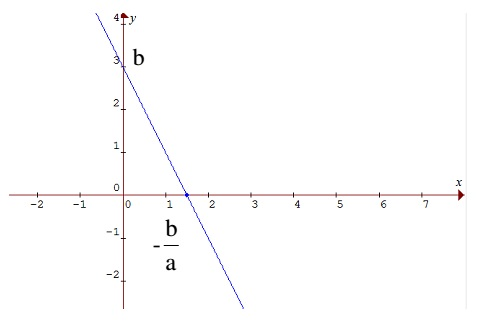
\includegraphics[height=5cm]{2_elem_rekenvaardigheden_B/inputs/eerstegraadsfuncties3.jpg}
%\caption{Voorbeeld grafische voorstelling van de eerstegraadfunctie.}
%\label{fig:eerste_vb_graf} 
%\end{figure}

Nulpunten:

We lossen de vergelijking $y=f(x)=-2x+3=0$ op en vinden:
$x=\frac{3}{2}$. Het snijpunt met de $x$-as is het punt $(\frac{3}{2},0)$.

Tekenverloop: zie Tabel \ref{tab:eerste_vb}.

\begin{tabel}{Voorbeeld eerstegraadsfunctie: tekenverloop}
\begin{tabular}{c||c|c|c}
	$x$ &  & $\frac{3}{2}$ & \\
	\hline 
	$f(x)$ & $+$ & 0 & $-$\\
\end{tabular}
\label{tab:eerste_vb}	
\end{tabel}

\end{voorbeeld}

\subsubsection{Tweedegraadsfuncties of kwadratische functies}



\begin{definitie}
	Functievoorschrift: $f(x)=ax^{2}+bx+c$ met $a\in\mathbb{R}_{0}$
en $b,c\in\mathbb{R}$ 

\end{definitie}

\begin{voorbeeld}
	$f(x)=3x^{2}+10x+1$ , $f(x)=-2x^{2}+5$
, $f(x)=x^{2}$
\end{voorbeeld}

Grafische voorstelling van de kwadratische functie
is een parabool.
%TODO figuur  vervangen 
\gewonefiguur{width=.7\linewidth}{2_elem_rekenvaardigheden_B/inputs/tweedegraadsfuncties1.jpg}

%\begin{figure}[h]
%\centering{}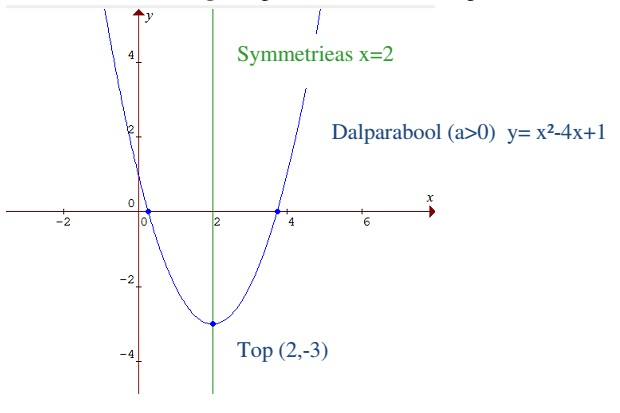
\includegraphics[width=.7\linewidth]{2_elem_rekenvaardigheden_B/inputs/tweedegraadsfuncties1.jpg}
%\caption{Grafische voorstelling van een tweedegraadsfunctie.}
%\label{fig:tweede} 
%\end{figure}

\begin{itemize}
\item als $a>0$ is de top van de \textbf{dalparabool} het minimum
\item als $a<0$ is de top van de \textbf{bergparabool} het maximum
\end{itemize}
Hoe groter de absolute waarde van $a$, hoe smaller de opening
van de parabool is.

De verticale lijn door de top is de \textbf{symmetrieas}.
De vergelijking van de symmetrieas is: $x=-\frac{b}{2a}$ 

Het laagste punt van een dalparabool of het hoogste punt
van een bergparabool heet de \textbf{top} van de parabool. De top
is het snijpunt van de parabool met de verticale symmetrieas. De co\"ordinaten
van de top zijn dus $(-\frac{b}{2a},y)$. De $y$-waarde vinden we
door de gevonden $x$-waarde in het functievoorschrift $f(x)$ in
te vullen, dus $y=f(-\frac{b}{2a})$ .

Nulpunten: stellen we $y=f(x)=ax^{2}+bx+c=0$
(in dat geval spreken we van de \textbf{vierkantsvergelijking}), dan
vinden we de snijpunten met de $x$-as. Hiervoor moeten we dus de
(vierkants)vergelijking $ax^{2}+bx+c=0$ oplossen. Daarvoor bepaal
je best eerst de \textbf{discriminant} $D=b^{2}-4ac$ (van de abc
formule). Met de discriminant bepaal je het aantal snijpunten van
de kwadratische functie met de $x$-as.
\begin{itemize}
\item als $D>0$ , dan heeft de vergelijking twee oplossing: $x_{1}=\frac{-b+\sqrt{D}}{2a}$
en $x_{2}=\frac{-b-\sqrt{D}}{2a}$. De parabool snijdt de $x$-as
op twee plaatsen.
\item als $D=0$ , dan heeft de vergelijking \'e\'en oplossing: $x_{1}=x_{2}=-\frac{b}{2a}$.
De parabool raakt met zijn top de $x$-as in \'e\'en punt.
\item als $D<0$ , dan heeft de vergelijking geen re\"ele oplossingen. De
parabool ligt ofwel boven ofwel onder de $x$-as.
\end{itemize}

%TODO figuur vervangen 
\gewonefiguur{scale=0.8}{2_elem_rekenvaardigheden_B/inputs/tweedegraadsfuncties2.jpg}

%\begin{figure}[h]
%\centering{}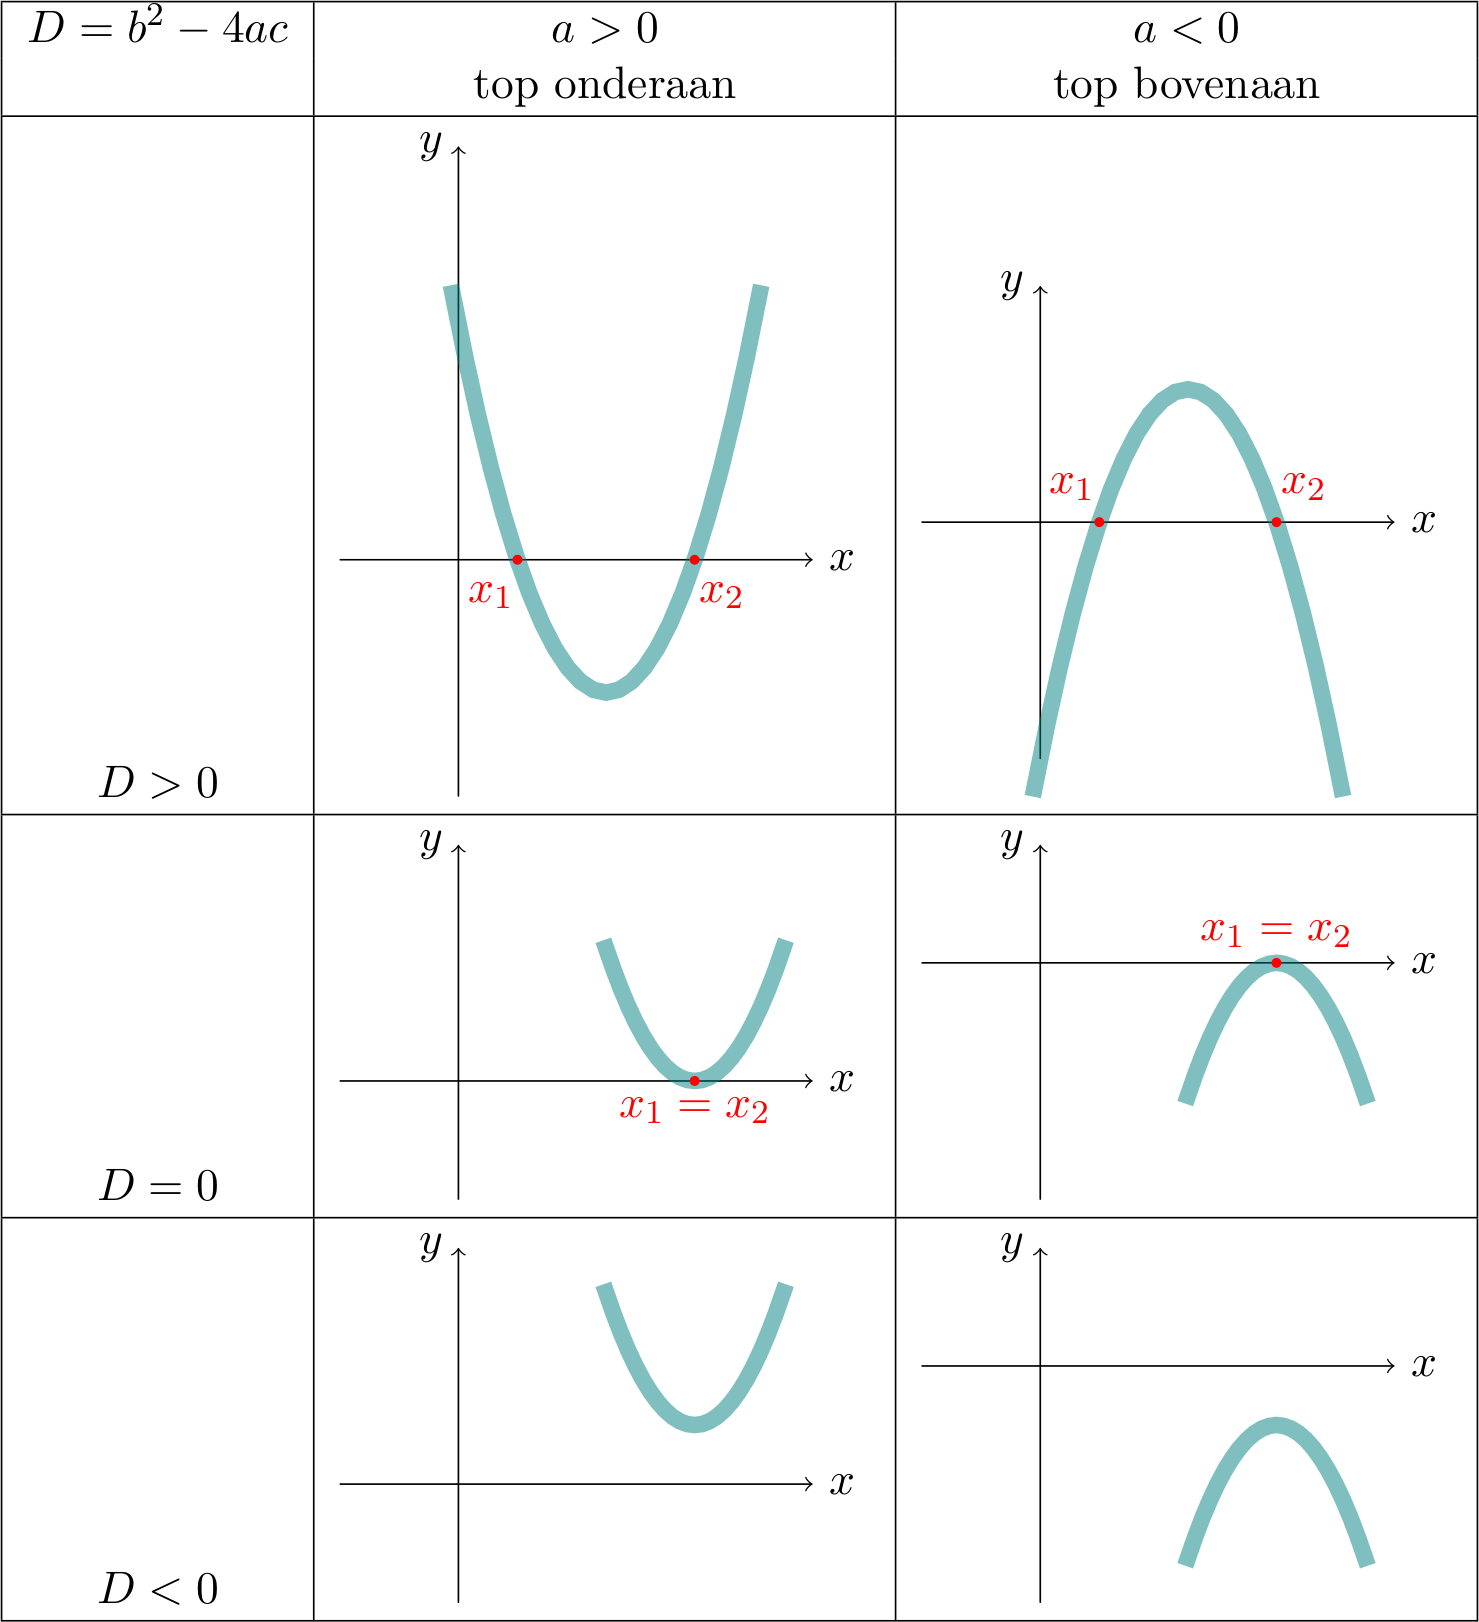
\includegraphics[scale=0.8]{2_elem_rekenvaardigheden_B/inputs/tweedegraadsfuncties2.jpg} 
%\caption{Grafische voorstelling van tweedegraadsfuncties voor verschillende waarden van $a$ en $D$.}
%\label{fig:tweede:gevallen}
%\end{figure}


%\uline{Opmerking}: stellen we de eerste afgeleide gelijk
%aan nul, dan vinden we de $x$-co\"ordinaat van de top: $f^{'}(x)=(ax^{2}+bx+c)^{'}=2ax+b=0$
%of $x=-\frac{b}{2a}$ . Het teken van de eerste afgeleide zegt ons
%of de functie (links en rechts van de top) stijgt of daalt. Tenslotte,
%het teken van de tweede afgeleide $f^{''}(x)=(2ax+b)^{'}=2a$, m.a.w.
%het teken van $a$ , zegt ons of het om een dal- of bergparabool gaat.

Tekenverloop:

\begin{itemize}
\item Als $D>0$ \\
\begin{center}
	\begin{tabular}{c||c|c|c|c|c}
$x$ &  & $x_{1}$ &  & $x_{2}$ & \\
\hline 
$f(x)$ & teken van $a$ & 0 & tegengesteld teken van $a$ & 0 & teken van $a$\\
\end{tabular}
\end{center}
\item Als $D=0$ \\
\begin{center}
	\begin{tabular}{c||c|c|c}
	$x$ &  & $x_{1}=x_{2}$ & \\
	\hline 
	$f(x)$ & teken van $a$ & 0 & teken van $a$\\
\end{tabular}
\end{center}
\item Als $D<0$ \\
\begin{center}
	\begin{tabular}{c||c}
$x$ & \\
\hline 
$f(x)$ & teken van $a$\\
\end{tabular}
\end{center}
\end{itemize}
%\begin{table}[h]
%\centering
%\caption{Algemeen tekenverloop van een tweedegraadsfunctie voor $D>0$}
%\end{table}
%\begin{tabular}{c|c}
%$D=0$ & %
%\begin{tabular}{c||c|c|c}
%$x$ &  & $x_{1}=x_{2}$ & \\
%\hline 
%\hline 
%$f(x)$ & teken van $a$ & 0 & teken van $a$\\
%\end{tabular}\\
% & \\
%\hline 
% & \\
%$D>0$ & %
%\begin{tabular}{c||c|c|c|c|c}
%$x$ &  & $x_{1}$ &  & $x_{2}$ & \\
%\hline 
%\hline 
%$f(x)$ & teken van $a$ & 0 & tegengesteld teken van $a$ & 0 & teken van $a$\\
%\end{tabular}\\
% & \\
%\hline 
% & \\
%$D<0$ & %
%\begin{tabular}{c||c}
%$x$ & \\
%\hline 
%\hline 
%$f(x)$ & teken van $a$\\
%\end{tabular}\\
%\end{tabular}


\begin{voorbeeld}
	Gegeven de functie $f$ met voorschrift: $f(x)=-x^{2}-5x+6$ 

Grafische voorstelling:
\begin{itemize}
\item het domein van elke kwadratische functie is: $\textrm{dom}f=\mathbb{R}$
\item $a=-1<0$ dus het is een bergparabool
\item de symmetrieas ligt bij $x=-\frac{b}{2a}=-\frac{-5}{2.(-1)}=-\frac{5}{2}=-2,5$
\item de top heeft de co\"ordinaten $(x,y)=(-\frac{b}{2a},f(-\frac{b}{2a}))=(-2,5;12,25)$
\item de top van deze bergparabool ligt op $y=12,25$. Dit is dus de grootste
waarde die $y$ kan bereiken. Het beeld van deze kwadratische functie
is daarom: $\textrm{bld}f=]-\infty;12,25]$
\end{itemize}


Nulpunten:

We lossen de vergelijking $y=f(x)=-x^{2}-5x+6=0$ op d.m.v.
de abc formule. We berekenen daarvoor eerst de discriminant $D$:

\begin{equation*}
D=b^{2}-4ac=(-5)^{2}-4.(-1).6=25+24=49
\end{equation*}

Omdat $D>0$ zijn er 2 re\"ele oplossingen, dus 2 snijpunten
met de $x$-as. Deze zijn:
\begin{itemize}
\item $x_{1}=\frac{-b+\sqrt{D}}{2a}=\frac{-(-5)+\sqrt{49}}{2.(-1)}=-6$
\item $x_{2}=\frac{-b-\sqrt{D}}{2a}=\frac{-(-5)-\sqrt{49}}{2.(-1)}=1$
\end{itemize}
De parabool snijdt de horizontale as in de koppels (-6,0) en (1,0)
en de top ligt boven de $x$-as (want het is een bergparabool).
%TODO figuur vervangen
\gewonefiguur{width=.5\linewidth}{2_elem_rekenvaardigheden_B/inputs/tweedegraadsfuncties3.jpg}

%\begin{figure}[h]
%\centering{}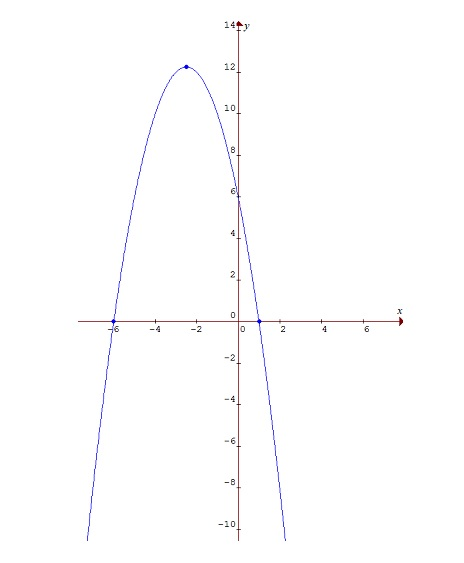
\includegraphics[width=.5\linewidth]{2_elem_rekenvaardigheden_B/inputs/tweedegraadsfuncties3.jpg}
%\caption{Voorbeeld tweedegraadsfuncties: grafische voorstelling}
%\label{fig:tweede:vb} 
%\end{figure}


Tekenverloop:


\begin{tabel}{Voorbeeld tweedegraadsfuncties: tekenverloop}
\begin{tabular}{c||c|c|c|c|c}
	$x$ &  & $-6$ &  & $1$ & \\
	\hline 
	$f(x)$ & $-$ & 0 & $+$ & 0 & $-$\\
\end{tabular}
\label{tab:tweede:vb}	
\end{tabel}

\end{voorbeeld}
\subsection{Tweedegraadsvergelijking - voorbeeld 1}
\begin{minipage}{.25\linewidth}
	\raggedright
	
\includegraphics[width=4cm]{2_elem_rekenvaardigheden_B/inputs/QR_Code_TWEEDEGRVGL1_module2new}
\end{minipage}
\begin{minipage}{.7\linewidth}
	Zie filmpje MOOC.
\end{minipage}
\subsection{Tweedegraadsvergelijking - voorbeeld 2}
\begin{minipage}{.25\linewidth}
	\raggedright
	
\includegraphics[width=4cm]{2_elem_rekenvaardigheden_B/inputs/QR_Code_TWEEDEGRVGL2_module2new}
\end{minipage}
\begin{minipage}{.7\linewidth}
	Zie filmpje MOOC.
\end{minipage}
%\input{2_elem_rekenvaardigheden_B/module_2_1_5}
%\input{2_elem_rekenvaardigheden_B/module_2_1_6}
%\subsection{Veeltermfuncties}

\subsubsection{Veeltermfuncties of polynoomfuncties}

\emph{Definitie}

Een veelterm- of polynoomfunctie heeft als functievoorschrift een veelterm in 1 onbekende, dus
$f(x)=a_{n}x^{n}+a_{n-1}x^{n-1}+\ldots+a_{2}x^{2}+a_{1}x+a_{0}$
met $a_{n}\in\mathbb{R}_{0}$ en $a_{n-1},\ldots,a_{0}\in\mathbb{R}$. De constanten $a_{i}$ noemen we de \textbf{co\"effici\"enten}.

De (meestal eerste) term met de hoogste macht bepaalt de \textbf{graad} van de veeltermfunctie.

\emph{Voorbeelden}

$f(x)=2x^{4}-5x^{3}+10x$ , $f(x)=x^{3}$ 

\textbf{Grafische voorstelling}

\noindent Het domein van een veeltermfunctie is: $\textrm{dom}f=\mathbb{R}$

\noindent De grafieken van de elementaire machtsfuncties $y=x^{n}$
met positieve exponent zijn hieronder weergegeven:

\begin{figure}[h]
\centering{}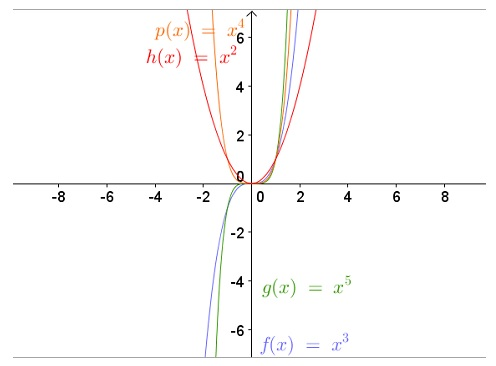
\includegraphics[height=5cm]{2_elem_rekenvaardigheden_B/inputs/veeltermfuncties1.jpg} 
\end{figure}


\noindent De grafieken van de elementaire machtsfuncties $y=x^{-n}=\frac{1}{x^{n}}$
met negatieve exponent zijn hieronder weergegeven:

\begin{figure}[h]
\centering{}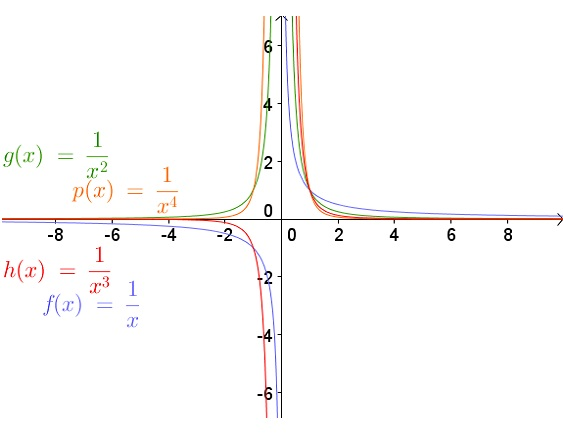
\includegraphics[height=5cm]{2_elem_rekenvaardigheden_B/inputs/veeltermfuncties2.jpg} 
\end{figure}


\textbf{Nulwaarden}

\noindent Een $n$\textsuperscript{de} graadsveeltermfunctie met oneven
$n$ heeft minimum $1$ en maximum $n$ snijpunten met de $x$-as.

\noindent Een $n$\textsuperscript{de} graadsveeltermfunctie met even
$n$ heeft minimum $0$ en maximum $n$ snijpunten met de $x$-as. De grafiek
kan namelijk helemaal boven of onder de $x$-as liggen, en dus geen
snijpunten hebben met de $x$-as.

\emph{Voorbeeld}

De functie $f$ met voorschrift $f(x)=2x^{4}-3x^{3}-x^{2}+x$ uit Figuur \ref{fig:vt:vb1}
is een 4\textsuperscript{de} graadsvergelijking en heeft in dit geval
4 snijpunten met de $x$-as:

\begin{figure}[h]
\centering{}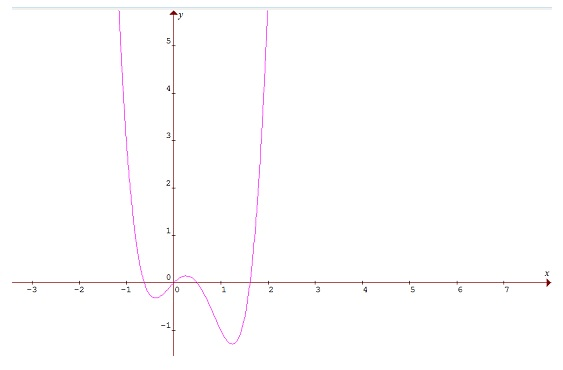
\includegraphics[height=5cm]{2_elem_rekenvaardigheden_B/inputs/veeltermfuncties3.jpg} 
\caption{Voorbeeld veeltermfunctie.}
\label{fig:vt:vb1}
\end{figure}

\textbf{Nulwaarden vinden}

De nulwaarden voor een veeltermfunctie vinden we door het
functievoorschrift te ontbinden in een product van factoren met ten
hoogste een tweede graad, m.a.w. we ontbinden de veeltermfunctie $f(x)$
in lineaire factoren $x+a$ en in kwadratische factoren $ax^{2}+bx+c$.
De nulpunten van de functie $f(x)$ zijn dan de nulpunten van de verschillende
factoren.

\textbf{Tekenverloop}

Eens een veelterm ontbonden is in factoren, is het eenvoudig
om het tekenverloop er van te bepalen. Het tekenverloop van een constante,
een lineaire en een kwadratische functie is immers gekend. Het teken
van een veeltermfunctie is het product van de tekens van de factoren.


\emph{Voorbeeld (een tweedegraadsfunctie verleiden door substitutie)}

Deze methode is toepasbaar bij bikwadratische vergelijkingen. Dit
zijn vergelijkingen van de vorm $ax^{4}+bx^{2}+c=0$. Dit type van
vergelijkingen kan herleid worden tot een kwadratische vergelijking
met behulp van de substitutiemethode. Stel hierbij $x^{2}=t$.

We bekijken de veelterm $f(x)=4x^{4}-5x^{2}+1$

\textbf{Nulwaarden}

\noindent We bepalen de nulwaarden door de veelterm te ontbinden in
factoren, gebruik makend van de substitutiemethode:\\

\begin{equation*}
4x^{4}-5x^{2}+1=0  \underrightarrow{x^{2}=t}  4t^{2}-5t+1=0
\end{equation*}

\noindent We bekomen een kwadratische vergelijking. Hiervan zijn de
nulpunten:
\begin{eqnarray*}
t_{1}=\frac{-b+\sqrt{D}}{2a}&=&\frac{-(-5)+\sqrt{9}}{2.4}=1 \\
t_{2}=\frac{-b-\sqrt{D}}{2a}&=&\frac{-(-5)-\sqrt{9}}{2.4}=\frac{1}{4}
\end{eqnarray*}

De 2 oplossingen voor $t$ zijn $t_{1}=1$ en $t_{2}=\frac{1}{4}$
zodat de vergelijking kan geschreven worden als: $4t^{2}-5t+1=(t-1)(t-\frac{1}{4})$.

Aangezien $x^{2}=t$ zijn de 4 oplossingen voor $x$: $x_{1en2}=\pm\sqrt{t_{1}}$
en $x_{3en4}=\pm\sqrt{t_{2}}$ 

Dit geeft $x_{1}=1$ , $x_{2}=-1$ , $x_{3}=\frac{1}{2}$
en $x_{4}=-\frac{1}{2}$.

De gegeven vergelijking kan dus ook geschreven worden als:

\begin{equation*}
f(x)=4x^{4}-5x^{2}+1=(x-1)(x+1)(x-\frac{1}{2})(x+\frac{1}{2})
\end{equation*}

\textbf{Tekenverloop}

Maak \'e\'en overzichtelijke tabel met bovenaan alle nulpunten
in stijgende volgorde. Per rij onderzoek je het teken van elke factor
van $f(x)$. Het teken van $f(x)$ is dan het product van deze tekens.

\begin{center}
\begin{tabular}{c||ccccccccc}
$x$ &  & $-1$ &  & $-\frac{1}{2}$ &  & $\frac{1}{2}$ &  & $1$ & \\
\hline 
$(x-1)$ & - & - & - & - & - & - & - & $0$ & $+$\\
$(x-\frac{1}{2})$ & - & - & - & - & -  & $0$ & + & + & + \\
$(x+\frac{1}{2})$ & - & - & - & $0$ & + & + & + & + & + \\
$(x+1)$ & $-$ & $0$ & + & + & + & + & + & + & + \\
\hline 
$f(x)$ & $+$ & $0$ & $-$ & $0$ & $+$ & $0$ & $-$ & $0$ & $+$\\
\end{tabular}
\end{center}


\emph{Voorbeeld 2 (ontbinden in factoren)}

We bekijken de veelterm $f(x)=3x^{3}-4x^{2}-6x+8$

\textbf{Nulpunten}

We bepalen de nulpunten door de veelterm te ontbinden in
factoren. Soms kunnen we gebruik maken van merkwaardige producten
of, zoals in dit geval, door het groeperen van gemeenschappelijke
termen:

\begin{eqnarray*}
3x^{3}-4x^{2}-6x+8 & = & (3x^{3}-4x^{2})-(6x-8)\\
 & = & x^{2}(3x-4)-2(3x-4)\\
 & = & (x^{2}-2)(3x-4)\\
 & = & (x-\sqrt{2})(x+\sqrt{2})(3x-4)
\end{eqnarray*}

\noindent De gegeven vergelijking $3x^{3}-4x^{2}-6x+8=0$ heeft dus
3 nulpunten:

\begin{equation*}
x_{1}=\sqrt{2}, x_{2}=-\sqrt{2} \text{ en } x_{3}=\frac{4}{3}
\end{equation*}

\textbf{Tekenverloop}

Maak \'e\'en overzichtelijke tabel met bovenaan alle nulpunten
in stijgende volgorde. Per rij onderzoek je het teken van elke factor
van $f(x)$. Het teken van $f(x)$ is dan het product van deze tekens.

\begin{center}
\begin{tabular}{c||ccccccc}
$x$ &  & $-\sqrt{2}$ &  & $\frac{4}{3}$ &  & $\sqrt{2}$ & \\
\hline 
$(x-\sqrt{2})$ & - & - & -& -& - & $0$ & $+$ \\
$(x+\sqrt{2})$ & $-$ & $0$ & + & + & +&+&+ \\
$(3x-4)$ & - & - & - & $0$ & +&+&+ \\
\hline 
$f(x)$ & $-$ & $0$ & $+$ & $0$ & $-$ & $0$ & + \\
\end{tabular}
\end{center}


\emph{Voorbeeld 3 (regel van Horner)}

We bekijken de veelterm $f(x)=x^{4}-4x^{3}+5x^{2}-4x+4$

\textbf{Nulpunten}

We bepalen de nulpunten door de veelterm te ontbinden in
factoren gebruik makend van de regel van Horner.

Ga na welke mogelijke delers van $a_{0}$ kunnen afgesplitst
worden zonder rest. Hier zijn de delers van $a_{0}=4$: $\pm1,\:\pm2\:\textrm{en}\:\pm4$

We proberen $x=+2$: $f(2)=(2)^{4}-4(2)^{3}+5(2)^{2}-4(2)+4=0$

Dus de factor $(x-2)$ kan afgesplitst worden. De co\"effici\"enten
van de resterende veelterm vinden we via de regel van Horner:

\begin{center}
\begin{tabular}{r||rrrrr}
	& $1$ & $-4$ & $5$ & $-4$ & $4$\\
	$\mathbf{2}$ & $\downarrow$ & $2$ & $-4$ & $2$ & $-4$\\
	\hline  
	& $1$ & $-2$ & $1$ & \multicolumn{1}{r|}{$-2$} & $\mathbf{0}$\\
\end{tabular}	
\end{center}

We vinden $f(x)=x^{4}-4x^{3}+5x^{2}-4x+4=(x-2)(x^{3}-2x^{2}+x-2)$

We kunnen proberen om nog een factor af te splitsten.

We proberen nog eens $x=+2$: $f(2)=(2)^{3}-2(2)^{2}+(2)-2=0$

Dus de factor $(x-2)$ kan nog eens afgesplitst worden.
De co\"effici\"enten van de resterende veelterm vinden we terug via de
regel van Horner:

\begin{center}
\begin{tabular}{r||rrrr}
	& $1$ & $-2$ & $1$ & $-2$\\
	$\mathbf{2}$ & $\downarrow$ & $2$ & $0$ & $2$\\
	\hline 
	& $1$ & $0$ & \multicolumn{1}{r|}{$1$} & $\mathbf{0}$\\
\end{tabular}
\end{center}

We vinden tenslotte: $f(x)=x^{4}-4x^{3}+5x^{2}-4x+4=(x-2)^{2}(x^{2}+1)$

Merk op dat de discriminant $D$ van $(x^{2}+1)$ negatief
is zodat deze factor geen nulpunten heeft.

We vinden voor $x=2$ een dubbel nulpunt; deze veelterm
heeft dus 2 samenvallende snijpunten met de $x$-as.

Aangezien zowel de factor $(x-2)^{2}$ als ook de factor
$(x^{2}+1)$ steeds positief zijn, is er voor geen enkele waarde van
$x$ een negatief beeld (de functie bevindt zich overal boven de $x$-as,
en in het punt $x=2$ raakt deze veelterm de $x$-as),zie ook Figuur \ref{fig:vt:vb4}.

\begin{figure}[h]
\centering{}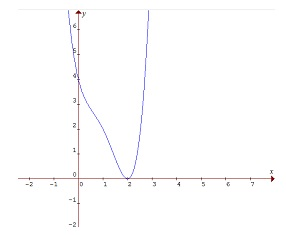
\includegraphics[width=.6\linewidth]{2_elem_rekenvaardigheden_B/inputs/veeltermfuncties4.jpg} 
\caption{Veeltermfuncties: voorbeeld 4.}
\label{fig:vt:vb4}
\end{figure}


\textbf{Tekenverloop}

Maak \'e\'en overzichtelijke tabel met bovenaan alle nulpunten
in stijgende volgorde. Per rij onderzoek je het teken van elke factor
van $f(x)$. Het teken van $f(x)$ is dan het product van deze tekens.

\begin{center}
\begin{tabular}{c||c|c|c}
$x$ &  & $2$ & \\
\hline 
$(x-2)^{2}$ & $+$ & $0$ & \multicolumn{1}{c}{$+$}\\
$(x^{2}+1)$ & +&+&+\\
\hline 
$f(x)$ & $+$ & $0$ & $+$\\
\end{tabular}
\par\end{center}

%\subsection{Rationale functies}

\begin{definitie}
	Functievoorschrift

${\displaystyle f(x)=\frac{t(x)}{n(x)}}$ met $t(x)$ en $n(x)$ veeltermfuncties
en waarbij de graad van $n(x)$ minstens 1 is.
\end{definitie}

\begin{voorbeeld}
Voorbeelden van rationale functies: ${\displaystyle f(x)=\frac{x^{2}}{1+x}}$,
${\displaystyle f(x)=\frac{1}{x^{2}-1}}$, ${\displaystyle f(x)=\frac{3x-9}{x-3}}$

Voorbeelden van niet-rationale functies: ${\displaystyle f(x)=\frac{\sin x}{4x}}$,
${\displaystyle f(x)=\frac{2^{x}}{3x+5}}$, ${\displaystyle f(x)=\frac{\sqrt{x-1}}{x-3}}$

\end{voorbeeld}

\textbf{Grafische voorstelling}

Het domein van een rationale functie is $\mathbb{R\setminus}\textrm{\{nulpunten\:van\:de\:noemer\}}$.

\begin{definitie}
	Voorbeeld: het domein van ${\displaystyle f(x)=\frac{2x+2}{x-8}}$
is ${\displaystyle \mathbb{R}\setminus\{8\}}$
\end{definitie}

\textbf{Nulpunten}

De nulpunten van een rationale functie $f(x)$, zijn de nulpunten
van de teller, die niet de nulpunten van de noemer zijn.

De nulpunten van de noemer, noemen we de polen van de rationale functie
$f(x)$. Bij elke pool hoort een verticale asymptoot.

Punten die zowel nulpunt zijn van teller als noemer, geven aanleiding
tot de vorm $\frac{0}{0}$. Aangezien deze punten de noemer nul maken,
horen ze niet tot het domein, maar geven ook geen aanleiding tot een
asymptoot.


\textbf{Asymptoten}

\begin{enumerate}
\item De rechte $x=a$ is een \textbf{verticale asymptoot} (VA) van de
rationale functie $f(x)$ als en slechts als $a$ een nulpunt is van
de noemer en geen nulpunt van de teller.

\begin{equation*}
\lim_{\overset{x\rightarrow a}{<}}f(x)=\pm\infty\quad\textrm{of}\quad \lim_{\overset{x\rightarrow a}{>}}f(x)=\pm\infty \\
		\Rightarrow\:x=a\:\textrm{is een VA}
\end{equation*}

\begin{voorbeeld}
\ 
\begin{equation*}
f(x)=\frac{2x+1}{x-1}
\end{equation*}

Het nulpunt van de noemer, of de pool is $x=1$. Dit punt is geen
nulpunt van de teller. Dus, $x=1$ is een verticale asymptoot. De
functie $f(x)$ is niet gedefinieerd in het punt $x=1$.
\begin{equation*}
\lim_{\overset{x\rightarrow1}{<}}\left(\frac{2x+1}{x-1}\right)=-\infty\quad\textrm{en}\quad \lim_{\overset{x\rightarrow1}{>}}\left(\frac{2x+1}{x-1}\right)=+\infty
\Rightarrow\:x=1\:\textrm{is een VA}
\end{equation*}

\end{voorbeeld}

\item Een rationale functie $f(x)$ heeft een \textbf{horizontale asymptoot}
(HA) als en slechts als de graad van de teller \ensuremath{\le} graad
van de noemer.

\begin{equation*}
\lim_{x\to\pm\infty}f(x)=b
\Rightarrow\:y=b\:\textrm{is een HA}
\end{equation*}

\begin{voorbeeld}
\ 
\begin{equation*}
f(x)=\frac{2x+7}{4x^{2}+x+2}
\end{equation*}

De graad van de teller is 1, en de graad van de noemer is 2; dus deze
functie heeft een horizontale asymptoot.

\begin{equation*}
\lim_{x\to\pm\infty}\frac{2x+7}{4x^{2}+x+2}\overset{HGT}{=} \lim_{x\to\pm\infty}\frac{2x}{4x^{2}}=\lim_{x\to\pm\infty}\frac{1}{2x}=0
\displaystyle \Rightarrow\:y=0\:\textrm{is een HA}
\end{equation*}

\end{voorbeeld}

\item Een rationale functie $f(x)$ heeft een \textbf{schuine asymptoot}
(SA) als en slechts als de graad van de teller = graad van de noemer
+1.

\begin{equation*}
m=\lim_{x\to\pm\infty}\frac{f(x)}{x}\quad\textrm{en}\quad q=\lim_{x\to\pm\infty}\left[f(x)-mx\right]\Rightarrow\:y=mx+q\:\textrm{is een SA}
\end{equation*}

\begin{voorbeeld}
	\begin{equation*}
f(x)=\frac{x^{3}-4}{2x^{2}}
\end{equation*}

De graad van de noemer is 2, en de graad van de teller is (2+1=) 3,
dus deze functie heeft een schuine asymptoot.

\begin{eqnarray*}
m&=&\lim_{x\to\pm\infty}\frac{f(x)}{x}= \lim_{x\to\pm\infty}\frac{x^{3}-4}{2x^{3}}\overset{HGT}{=} \lim_{x\to\pm\infty}\frac{x^{3}}{2x^{3}}=\frac{1}{2}
\\
q&=& \lim_{x\to\pm\infty}\left[\frac{x^{3}-4}{2x^{2}}-\frac{1}{2}x\right]=\lim_{x\to\pm\infty}\left[\frac{x^{3}-4-x^{3}}{2x^{2}}\right]=0 \\
&&\Rightarrow\:y=\frac{1}{2}x\:\textrm{is een SA}
\end{eqnarray*}

\end{voorbeeld}

\begin{opmerking}
Als een functie $f(x)$ voor $x\rightarrow+\infty$ een
horizontale asymptoot heeft, kan ze voor $x\rightarrow+\infty$ geen
schuine asymptoot meer hebben. Hetzelfde geldt voor $x\rightarrow-\infty$.
\end{opmerking}
\end{enumerate}

\textbf{Tekenverloop}

Om het tekenverloop van een rationale functie te bepalen, moet het
tekenonderzoek van de teller en de noemer worden uitgevoerd. Het tekenverloop
van een constante, een lineaire en een kwadratische functie is gekend
(zie Module 2 sectie \ref{sec:eerste_tweede} en \ref{sec:vtf}).
Het teken van de rationale functie is het product van het teken van
de teller en het teken van de noemer.


\begin{voorbeeld}
Bespreek de rationale functie 
\begin{equation*}
f(x)=\frac{3x^{2}}{x^{2}-2}
\end{equation*}

\underline{Domein}

$\textrm{dom}f(x)=\mathbb{R}\setminus\{-\sqrt{2},\sqrt{2}\}$ want de noemer mag niet nul worden. Dit gebeurt als ${\displaystyle x^{2}-2=0}\Longleftrightarrow x=\pm\sqrt{2}$.

\underline{Nulwaarden}

Stap 1: Bepaal de nulpunten van de teller, deze zijn de nulpunten
van de functie $f(x)$. Dus $3x^{2}=0\Longleftrightarrow x=0$ .

$x=0$ is een nulpunt van de teller, maar niet van de noemer, dus
dit punt is een nulpunt van de functie $f(x)$.

Stap 2: Bepaal de nulpunten van de noemer, deze zijn de polen van
de functie $f(x)$. Bij elke pool hoort een verticale asymptoot.

$x=-\sqrt{2}$ en $x=+\sqrt{2}$ zijn de nulpunten van de noemer,
de functie $f(x)$ heeft dus twee verticale asymptoten.

\underline{Asymptoten}

Stap 3: Ga na of de functie een verticale asymptoot bezit. 

De rechte $x=-\sqrt{2}$ is een verticale asymptoot (VA) van de functie
$f(x)$ aangezien $-\sqrt{2}$ een nulpunt is van de noemer en geen
nulpunt van de teller is.

Hoe verloopt de functie $f(x)$ in de buurt van deze asymptoot:

\begin{equation*}
\textrm{LL}: \lim_{\overset{x\rightarrow-\sqrt{2}}{<}}\left(\frac{3x^{2}}{x^{2}-2}\right)=+\infty\quad\textrm{en}\quad \textrm{RL}:\lim_{\overset{x\rightarrow-\sqrt{2}}{>}}\left(\frac{3x^{2}}{x^{2}-2}\right)=-\infty
\Rightarrow x=-\sqrt{2} \text{is een VA.}
\end{equation*}

De rechte $x=+\sqrt{2}$ is een verticale asymptoot (VA) van de functie
$f(x)$ aangezien $+\sqrt{2}$ een nulpunt is van de noemer en geen
nulpunt van de teller is.

Hoe verloopt de functie $f(x)$ in de buurt van deze asymptoot:

\begin{equation*}
\textrm{LL}: \lim_{\overset{x\rightarrow\sqrt{2}}{<}}\left(\frac{3x^{2}}{x^{2}-2}\right)=-\infty\quad\textrm{en}\quad \textrm{RL}:\lim_{\overset{x\rightarrow\sqrt{2}}{>}}\left(\frac{3x^{2}}{x^{2}-2}\right)=+\infty \\
\Rightarrow x=+\sqrt{2} \text{is een VA.}
\end{equation*}


Stap 4: Ga na of de functie een horizontale asymptoot bezit. De functie
$f(x)$ heeft een horizontale asymptoot (HA) aangezien de graad van
teller (2\textsuperscript{de} graad) = graad van de noemer (2\textsuperscript{de}
graad).

\begin{equation*}
\lim_{x\to\pm\infty}\frac{3x^{2}}{x^{2}-2}\overset{HGT}{=} \lim_{x\to\pm\infty}\frac{3x^{2}}{x^{2}}=3 \\
\Rightarrow y=3\text{ is een HA}.
\end{equation*}

Stap 5: Ga na of de functie een schuine asymptoot heeft. De functie
$f(x)$ heeft voor $x\rightarrow+\infty$ en $x\rightarrow-\infty$,
al een horizontale asymptoot en kan bijgevolg geen schuine asymptoot
meer hebben.

\underline{Tekenverloop}

Stap 6: - Schrijf in \'e\'en tabel bovenaan alle nulpunten en alle polen
in stijgende volgorde. 

\begin{itemize}
\item Onderzoek het teken voor elke factor van $f(x)$ . 
\item Het teken van $f(x)$ is dan het product van deze tekens.
\end{itemize}

\begin{center}
	\begin{tabular}{c||cccccccc} 
$x$ &  & $-\sqrt{2}$ &  & $0$ &  & $-\sqrt{2}$ &  & ${\displaystyle \longrightarrow\mathbb{R}}$\\
\hline 
${\displaystyle 3x^{2}}$ & + &  & + & 0 & + &  & + & \\
\hline 
${\displaystyle x^{2}-2}$ & + & 0 & - & - & - & 0 & + & \\
\hline 
${\displaystyle f(x)=\frac{3x^{2}}{x^{2}-2}}$ & + & $\mid$ & - & 0 & - & $\mid$ & + & \\
\end{tabular}
\end{center}

\underline{Grafiek}

%\gewonefiguur{width=10cm}{2_elem_rekenvaardigheden_B/inputs/vb_rat1}

\begin{figure}
\centering
\tikzsetfigurename{Fig_module_2_1_8_vb_rat1}
\begin{center}
\begin{tikzpicture}[xscale=1,yscale=0.5,cap=round]

% Styles
\tikzstyle{axes}=[]
\tikzstyle help lines=[color=blue!50,very thin,dotted]

% grid
\draw[style=help lines,step=1cm] (-7.9,-2.9) grid (7.9,9.9);

\draw[->] (-8,0) -- (8,0) node[right] {$x$};
\draw[->] (0,-3) -- (0,10) node[above] {$y$};

\draw[-,thin] (-1.41,-3)--(-1.41,10);

\draw[-,thin] (1.41,-3)--(1.41,10);


\draw[-,thin] (-7,3)--(7,3);
%\draw[fill,cyan](1,1)circle [radius=0.025];



%getallen op de x-as en lijntjes   
\foreach \x/\xtext in {-7,-6,-5,-4,-3,-2,-1,1,2,3,4,5,6,7}
\draw[xshift=\x cm] (0pt,1pt) -- (0pt,0pt) node[below,fill=white]
{$\xtext$};,3

%getallen op de y-as en lijntjes  
%BEGIN LUS
\foreach \y/\ytext in {-1,0,1,2,3,4,5,6,7,8,9}
\draw[yshift=\y cm] (1pt,0pt) -- (0pt,0pt) node[left,fill=white]
{$\ytext$}; %EINDE LUS



%FUNCTIEVOORSCHRIFTEN




\draw[blue,cap=rect,line width=1, opacity=1, domain=-7:-1.7,samples=100] plot (\x, {
	( 3*(pow(\x,2))) /(	pow(\x,2)-2)	% <- plaats het functievoorschrift hier	
}) node[opacity=1,above]{$$};
%-------------------------------------------


%---------------------------------------

\draw[blue,cap=rect,line width=1, opacity=1, domain=-1:1,samples=100] plot (\x, {
	( 3*(pow(\x,2))) /(	pow(\x,2)-2)	% <- plaats het functievoorschrift hier	
}) node[opacity=1,above]{$$};
%-------------------------------------------



\draw[blue,cap=rect,line width=1, opacity=1, domain=1.7:7,samples=100] plot (\x, {
	( 3*(pow(\x,2))) /(	pow(\x,2)-2)	% <- plaats het functievoorschrift hier	
}) node[opacity=1,above]{$$};
%-------------------------------------------


%legende





\end{tikzpicture}
\end{center}


\end{figure}


\end{voorbeeld}


\begin{ftonthoud}
	De grafiek en het tekenverloop van een rationale functie bepaal je
als volgt: $f(x)=\frac{t(x)}{n(x)}$ met $t(x)$ en $n(x)$ veeltermfuncties
en waarbij de graad van $n(x)$ minstens 1 is.

Het domein van een rationale functie is $\mathbb{R\setminus}\textrm{\{nulpunten\:van\:de\:noemer\}}$.

Stap 1: Bepaal de nulpunten van de teller, dit zijn de nulpunten van
de functie $f(x)$.

Stap 2: Bepaal de nulpunten van de noemer, dit zijn de polen van de
functie $f(x)$.

Stap 3: De rechte $x=a$ is een \textbf{verticale asymptoot} (VA)
van de rationale functie $f(x)$ als en slechts als $a$ een nulpunt
is van de noemer en maar geen nulpunt van de teller.

\begin{equation*}
\lim_{\overset{x\rightarrow a}{<}}f(x)=\pm\infty\quad\textrm{of}\quad \lim_{\overset{x\rightarrow a}{>}}f(x)=\pm\infty\quad\Rightarrow\:x=a\:\textrm{is een VA}
\end{equation*}


Stap 4: Een rationale functie $f(x)$ heeft een \textbf{horizontale
asymptoot} (HA) als en slechts als de graad van de teller \ensuremath{\le}
graad van de noemer. Maar hou wel rekening met het domein.

\begin{equation*}
\lim_{x\to\pm\infty}f(x)=b\quad\Rightarrow\:y=b\:\textrm{is een HA}
\end{equation*}

Stap 5: Een rationale functie $f(x)$ heeft een \textbf{schuine asymptoot}
(SA) als en slechts als de graad van de teller = graad van de noemer
+1. Maar hou wel rekening met het domein.

\begin{eqnarray*}
m= \lim_{x\to\pm\infty}\frac{f(x)}{x}\quad\textrm{en}\quad
q=\lim_{x\to\pm\infty}\left[f(x)-mx\right] \\
\Rightarrow\:y=mx+q\:\textrm{is een SA}
\end{eqnarray*}

Stap 6: Bepaal het tekenverloop
\begin{itemize}
\item Schrijf in \'e\'en tabel bovenaan alle nulpunten en alle polen in stijgende
volgorde. 

\item Onderzoek het teken voor elke factor van $f(x)$.

\item Het teken van $f(x)$ is dan het product van deze tekens.

\end{itemize}

\end{ftonthoud}

%\subsection{Irrationale functies}
%\maketitle
%\begin{itemize}
%\item Wat zijn irrationale functies?
%\item Wanneer hebben ze (verticale, horizontale en/of schuine) asymptoten?
%\end{itemize}
%Dit zijn vergelijkingen waarin wortelvormen voorkomen, eventueel met
%een breuk. Deze wortelvormen kan je wegwerken door beide leden van
%de vergelijking te verheffen tot een gepaste macht.

\begin{voorbeeld}
	$f(x)=\sqrt{x^{2}+2x+4}$, $f(x)=2\cdot \sqrt[3]{x^{5}-3x^{2}+7}-x-1$,
$f(x)=\frac{x-2}{\sqrt{10-x^{2}}}$
\end{voorbeeld}

\textbf{Grafische voorstelling}

De grafiek van de elementaire wortelfuncties $y=\sqrt[n]{x}$
is hieronder weergegeven. Denk eraan dat (machts)wortels ook als macht
kunnen geschreven worden: $y=\sqrt[n]{x}=x^{\frac{1}{n}}$.

\gewonefiguur{width=10cm}{2_elem_rekenvaardigheden_B/inputs/machtsw1}

Om het domein (de toegelaten waarden voor $x$) te bepalen moeten
we rekening houden met zowel de \emph{bestaansvoorwaarden} als de
\emph{kwadrateringsvoorwaarde}.

\begin{itemize}
	\item Bestaansvoorwaarde(n): de uitdrukking onder een even machtswortel
moet steeds positief zijn!! En niet vergeten, de eventuele noemer
mag niet nul worden.
\item Kwadrateringsvoorwaarde: we spreken af dat een even machtswortel uit
een uitdrukking steeds positief is.
\end{itemize}

Het domein van een irrationale functie valt samen met de intervallen,
waar de vorm onder de vierkantswortel niet negatief is en waar de
uitdrukking van een even machtsfunctie steeds een positief resultaat
oplevert.

\begin{voorbeeld}
	\begin{equation*}
f(x)=\sqrt{x^{2}-4}
\end{equation*}

\gewonefiguur{width=7cm}{2_elem_rekenvaardigheden_B/inputs/machtsw2}

Om het domein van de functie $f(x)$ te bepalen moet er aan de bestaansvoorwaarde(n)
voldaan zijn. In dit geval mag de functie onder het wortelteken niet
negatief worden. We werken dit verder uit:

De bestaansvoorwaarde: $\begin{array}{cccl}
x^{2}-4\geq0 &\iff & x^{2}\geq4\\
& \iff & x\geq2 \textrm{ en } x\leq-2
\end{array}$

De kwadrateringsvoorwaarde is reeds voldaan (want er staat infeite
$f(x)=+\sqrt{x^{2}-4}$).

Welke waarden van $x$ voldoen hier nu aan? $\textrm{dom}f(x)$ is voor $x\in]-\infty,-2]\bigcup[2,+\infty[$.

\end{voorbeeld}

\begin{voorbeeld}
\begin{equation*}
f(x)=x+\sqrt{5x+2}-1
\end{equation*}

\gewonefiguur{width=7cm}{2_elem_rekenvaardigheden_B/inputs/vbirrat1}

Om het domein van de functie $f(x)$ te bepalen moet er aan de bestaansvoorwaarde(n)
voldaan zijn. In dit geval mag de functie onder het wortelteken niet
negatief worden. We werken dit verder uit:

De bestaansvoorwaarde:$\begin{array}{cclccc}
 & 5x+2\geq0
 & \iff & x & \geq & -\frac{2}{5}\\
\textrm{dus} & & \iff & x & \in & [-\frac{2}{5},+\infty[
\end{array}$

Nu moeten we nog de kwadrateringsvoorwaarde controleren, m.a.w. volgens
onze gemaakte afspraak is een even machtswortel uit een uitdrukking
steeds positief is:

De bestaansvoorwaarde:
$\begin{array}{cccclcc}
 & x+\sqrt{5x+2}=1 & \iff & \sqrt{5x+2} & = & 1-x & \geq0\\
 & & \iff & 1-x & \geq & 0\\
\textrm{dus} & & \iff & x & \leq & 1\\
\textrm{of} & & \iff & x & \in & ]-\infty,1]
\end{array}$

De mogelijke waarden voor $x$ moeten aan beide voorwaarden voldoen.
Dit betekent: $\textrm{dom}f(x)$ is voor $x\in[-\frac{2}{5},1]$

\end{voorbeeld}

\textbf{Nulpunten}

De vergelijking wordt $f(x)=0$.

De wortelvormen kan je wegwerken door beide leden van de vergelijking
te verheffen tot een gepaste macht. Bepaal vervolgens de nulpunten
van de functie. Wanneer een breuk voorkomt in het functievoorschrift,
bepaal dan ook de nulpunten van de noemer, deze zijn de polen.

\textbf{Asymptoten}

\begin{enumerate}
	\item De rechte $x=a$ is een \textbf{verticale asymptoot} (VA) van de
irrationale functie $f(x)$ als en slechts als $a$ een nulpunt is
van de noemer en geen nulpunt van de teller.

\begin{equation*}
\lim_{\overset{x\rightarrow a}{<}}f(x)=\pm\infty\quad\textrm{of}\quad \lim_{\overset{x\rightarrow a}{>}}f(x)=\pm\infty \Rightarrow\:x=a\:\textrm{is een VA}
\end{equation*}

\item Een irrationale functie $f(x)$ heeft een \textbf{horizontale asymptoot}
(HA) als en slechts als de graad van de teller $\le$ graad
van de noemer.
\begin{equation*}
\lim_{x\to\pm\infty}f(x)=b \Rightarrow\:y=b\:\textrm{is een HA}
\end{equation*}

\item Een irrationale functie $f(x)$ heeft een \textbf{schuine asymptoot}
(SA) als en slechts als de graad van de teller = graad van de noemer
+1.

\begin{equation*}
m=\lim_{x\to\pm\infty}\frac{f(x)}{x}\quad\textrm{en}\quad 
q= \lim_{x\to\pm\infty}\left[f(x)-mx\right]
\Rightarrow\:y=mx+q\;\textrm{is een SA}
\end{equation*}

\end{enumerate}


\textbf{Tekenverloop}

Wanneer je de wortels hebt weggewerkt door de vergelijking te verheffen
tot een gepaste macht, zal je een veeltermfunctie, een kwadratische
of een lineaire functie bekomen. Pas het desbetreffend tekenonderzoek
toe.


\begin{voorbeeld}
	Bespreek de irrationale functie $f(x)=\frac{\sqrt{4-x^{2}}}{x-1}$

\underline{Domein}

\begin{eqnarray}
\textrm{dom}f(x)=[-2,1[\bigcup]1,2]
\end{eqnarray}

want de bestaansvoorwaarden zijn:  
\begin{equation*}
\begin{array}{ccclcc}
& 4-x^{2}\geq0 & \iff & x^{2}\leq4\\
\textrm{dus} & & \iff & x\leq2\;\textrm{en}\:x\geq-2\\
\textrm{of} & & \iff & x\in[-2,2]
\end{array}
\end{equation*}

en:
\begin{equation*}
x-1\neq0 \textrm{ dus } x\neq1
\end{equation*}

De kwadrateringsvoorwaarde is hier niet van toepassing (vanwege de
noemer kan $f(x)$ ook negatief worden).

\underline{Nulpunten}

Stap 1: Bepaal de nulpunten van de teller, deze zijn de nulpunten
van de functie $f(x)$.

Dus 
\begin{equation*}
\begin{array}{ccc}
f(x)=0 & \iff & \frac{\sqrt{4-x^{2}}}{x-1} = 0\\
& \iff & \sqrt{4-x^{2}} = 0\\
& \iff & 4-x^{2} = 0\\
& \iff & x^{2} = 4\\
& \iff & x = \pm2
\end{array}
\end{equation*}

Stap 2: Bepaal eventueel de nulpunten van de noemer, deze zijn de
polen van de functie $f(x)$. Bij elke pool hoort een verticale asymptoot.

Het nulpunt van de noemer is $x=1$ (dit is dan tevens de vergelijking
van de verticale asymptoot).

\underline{Asymptoten}

Stap 3: Ga na of de functie een verticale asymptoot bezit. 

De rechte $x=1$ is een verticale asymptoot (VA) van de functie $f(x)$
aangezien $1$ een nulpunt is van de noemer en geen nulpunt van de
teller is.

Hoe verloopt de functie $f(x)$ in de buurt van deze asymptoot:

\begin{equation*}
\textrm{LL}:\lim_{\overset{x\rightarrow1}{<}}\left(\frac{\sqrt{4-x^{2}}}{x-1}\right)=-\infty\quad\textrm{en}\quad \textrm{RL}:\lim_{\overset{x\rightarrow1}{>}}\left(\frac{\sqrt{4-x^{2}}}{x-1}\right)=+\infty \Rightarrow x=1 \text{ is een VA}
\end{equation*}


Stap 4: Ga na of de functie een horizontale asymptoot bezit.

De functie heeft geen horizontale asymptoot, want $x$ die nadert
naar $+\infty$ of $-\infty$ behoort niet tot het domein.

Stap 5: Ga na of de functie een schuine asymptoot heeft.

De functie heeft geen schuine asymptoot, want $x$ die nadert naar
$+\infty$ of $-\infty$ behoort niet tot het domein.

\underline{Tekenverloop}

Stap 6:
\begin{itemize}
\item Schrijf in \'e\'en tabel bovenaan alle nulpunten en alle polen
	in stijgende volgorde. 
\item Onderzoek het teken voor elke factor van $f(x)$. 
\item Het teken van $f(x)$ is dan het product van deze tekens.
\end{itemize}


\begin{tabel}{Voorbeeld irrationale functies: tekenverloop.}
\begin{tabular}{c|cccccccc}
$x$ &  & $-2$ &  & $1$ &  & $2$ &  & $\longrightarrow\mathbb{R}$\\
\hline  
$\sqrt{4-x^{2}}$ & / & 0 & + &  & + & 0 & / & \\
$x-1$ & - & - & - & 0 & + & + & + & \\
\hline 
$f(x)=\frac{\sqrt{4-x^{2}}}{x-1}$ & / & 0 & - & $\mid$ & + & 0 & / & \\
\end{tabular}
\label{tab:irrattk}
\end{tabel}

\underline{Grafiek}

\gewonefiguur{width=7cm}{2_elem_rekenvaardigheden_B/inputs/vbirrat2}

\end{voorbeeld}

\begin{ftonthoud}
	De grafiek en het tekenverloop van een irrationale functie bepaal
je als volgt:

Het domein van een irrationale functie valt samen met de intervallen,
waar de vorm onder de vierkantswortel niet negatief (BVW) is en waar
de uitdrukking van een even machtsfunctie steeds een positief resultaat
oplevert (KVW).

Stap 1: Bepaal de nulpunten van de teller, dit zijn de nulpunten van
de functie $f(x)$.

Stap 2: Bepaal eventueel de nulpunten van de noemer, dit zijn de polen
van de functie $f(x)$.

Stap 3: De rechte $x=a$ is een \textbf{verticale asymptoot} (VA)
van de irrationale functie $f(x)$ als en slechts als $a$ een nulpunt
is van de noemer en maar geen nulpunt van de teller.

\begin{equation*}
\lim_{\overset{x\rightarrow a}{<}}f(x)=\pm\infty\quad\textrm{of}\quad \lim_{\overset{x\rightarrow a}{>}}f(x)=\pm\infty\quad\Rightarrow\:x=a\:\textrm{is een VA}
\end{equation*}

Stap 4: Een irrationale functie $f(x)$ heeft een \textbf{horizontale
asymptoot} (HA) als en slechts als de graad van de teller \ensuremath{\le}
graad van de noemer.
\begin{equation*}
 \lim_{x\to\pm\infty}f(x)=b\quad\Rightarrow\:y=b\:\textrm{is een HA}
\end{equation*}


Stap 5: Een irrationale functie $f(x)$ heeft een \textbf{schuine
asymptoot} (SA) als en slechts als de graad van de teller = graad
van de noemer +1.

\begin{equation*}
m=\lim_{x\to\pm\infty}\frac{f(x)}{x}\quad\textrm{en}\quad q= \lim_{x\to\pm\infty}\left[f(x)-mx\right] \Rightarrow\:y=mx+q\:\textrm{is een SA}
\end{equation*}


Stap 6: Bepaal het tekenverloop

\begin{itemize}
\item Schrijf in \'e\'en tabel bovenaan alle nulpunten en alle polen in stijgende
volgorde.

\item Hou rekening met de bestaansvoorwaarde en de kwadrateringsvoorwaarde.

\item Onderzoek het teken voor elke factor van $f(x)$.

\item Het teken van $f(x)$ is dan het product van deze tekens.
\end{itemize}

\end{ftonthoud}
%%\DeclareMathOperator{\tri}{tri} \DeclareMathOperator{\rect}{rect}
%\DeclareMathOperator{\sgn}{sgn} \DeclareMathOperator{\ramp}{ramp}
%\DeclareMathOperator{\sinc}{sinc}


\subsection{Exponenti\"ele functies}
%\maketitle
%\begin{itemize}
%\item Wat is een exponenti\"ele functie?
%\item Hoe ziet het functievoorschrift van een exponenti\"ele functie eruit?
%\item Welke rekenregels voor machten en wortels zijn er?
%\item Hoe lossen we exponenti\"ele vergelijkingen op?
%\item Hoe kan je een exponenti\"ele functie grafisch voorstellen?
%\item Hoe bepaal je het tekenverloop van een exponenti\"ele functie? 
%\end{itemize}


\begin{definitie}
De exponenti\"ele functie is van de vorm:
\begin{equation*}
	y=a^{x}\text{ met }a\in\mathbb{R}_{0}^{+}\setminus\{ 1\}\text{ en }x\in\mathbb{R}
\end{equation*}
$a$ noemen we het \textbf{grondtal}, en moet strikt positief
en verschillend van 1 zijn.

$x$ noemen we de \textbf{exponent}, en is een re\"eel getal.
\end{definitie}

\begin{voorbeeld}
\begin{eqnarray*}
4^{2}&=&16 \\
3^{-2}&=&\frac{1}{3^{2}}=\frac{1}{9} \\
5^{\frac{2}{3}}&=&\sqrt[3]{5^{2}} \\
5^{-\frac{3}{2}}&=&\frac{1}{5^{\frac{3}{2}}}=\frac{1}{\sqrt{5^{3}}}=\frac{1}{\sqrt{5^{2}.5}}=\frac{1}{5\sqrt{5}}\\
\sqrt{25}&=&5 \\
\sqrt[4]{10000}&=&10\\
\sqrt[5]{-32}&=&-2\\
\sqrt[3]{8}&=&2\\
\end{eqnarray*}
\end{voorbeeld}

\begin{opmerking}
De positieve tweedemachts- of vierkantswortel van 25 is 5, want $5>0$ en $5^{2}=25$, dit wordt genoteerd als ${\displaystyle \sqrt{25}=5}$.

En de negatieve tweedemachts- of vierkantswortel van 25 is -5, want
$-5 < 0$ en $(-5)^{2}=25$, dit wordt genoteerd als ${\displaystyle -\sqrt{25}=-5}$.

Ook je rekenmachine zal bij ${\displaystyle \sqrt{25}}$ als resultaat
5 geven. Verwar dit niet met het oplossen van de vergelijking $x^{2}=25$.
In dit geval zijn de twee oplossingen van de vergelijking: $x=\pm\sqrt{25}=\pm5$.
\end{opmerking}

\subsubsection{Bijzondere gevallen}
\begin{itemize}
\item De exponenti\"ele functie met grondtal $e$ ($e=2,718281828$) wordt
genoteerd als $y=e^{x}$.
\item $a^{0}=1$
\item $a^{1}=a$
\item Als n even is spreekt men van een \emph{evenmachtswortel} ($\sqrt{\ }$,
$\sqrt[4]{\ }$, ...), is n oneven dan spreekt men van een \emph{onevenmachtswortel}
($\sqrt[3]{\ }$, $\sqrt[5]{\ }$, ...).
\item Positieve re\"ele getallen hebben twee tegengestelde evenmachtswortels
en juist \'e\'en positieve onevenmachtswortel.
\item als n even is, dan heeft elk re\"eel getal $a$ twee n\textsuperscript{de}
machtswortels die tegengesteld zijn, genoteerd door $-\sqrt[n]{a}$
en $+\sqrt[n]{a}$, of kortweg $\pm\sqrt[n]{a}$.
\item als n oneven is, dan heeft elk re\"eel getal a juist \'e\'en n\textsuperscript{de}
machtswortel, genoteerd door $\sqrt[n]{a}$.
\item Als n even is, dan hebben de negatieve getallen geen n\textsuperscript{de}
machtswortel; dus negatieve re\"ele getallen hebben geen (re\"ele) evenmachtswortel
en juist \'e\'en onevenmachtswortel welke negatief is.
\end{itemize}
Let op: worteltrekken is niet hetzelfde als het oplossen van een vergelijking:

\begin{tabel}{}
\begin{tabular}{c|c}
worteltrekken & vergelijking oplossen\\
\hline 
$\sqrt{4}=2$ & $\begin{array}{lll}
x^{2} & = & 4\\
x & = & \pm\sqrt{4}\\
x & = & \pm2
\end{array}$\\
\hline 
 &  $x_{1}=-2$ en $x_{2}=+2$\\
\end{tabular}
\end{tabel}


\subsubsection{Rekenregels}

\begin{tabel}{}
\begin{tabular}{l|l}
machten & wortels\\
\hline 
$a^{m}a^{n}=a^{m+n}$ & $\sqrt[m]{a}\cdot\sqrt[n]{a}=\sqrt[m\cdot n]{a^{m+n}}$\\
$\frac{a^{m}}{a^{n}}=a^{m-n}$ & $\sqrt[n]{a^{m}}=a^{\frac{m}{n}}$\\
$\left(\frac{1}{a}\right)^{n}=a^{-n}$ & $\sqrt[n]{a}=a^{\frac{1}{n}}$\\
$\left(a^{m}\right)^{n}=a^{m\cdot n}$ & $\sqrt[n]{\sqrt[m]{a}}=\sqrt[n\cdot m]{a}$\\
$\left(a\cdot b\right)^{n}=a^{n}\cdot b^{n}$ & $\sqrt[n]{a\cdot b}=\sqrt[n]{a}\cdot \sqrt[n]{b}$\\
$\left(\frac{a}{b}\right)^{n}=\frac{a^{n}}{b^{n}}$ & $\sqrt[n]{\frac{a}{b}}=\frac{\sqrt[n]{a}}{\sqrt[n]{b}}$\\
\end{tabular}
\end{tabel}


\begin{opmerking}
	\ \\
	\begin{itemize}
\item aangezien $1=\frac{a}{a}=a^{1-1}=a^{0}$ zie je waarom
we zeggen dat $a^{0}=1$.
\item formules met wortels kan je (gemakkelijk) terugvinden als je de wortelvorm
herschrijft d.m.v. machten:
\end{itemize}
\begin{equation*}
\sqrt[m]{a}.\sqrt[n]{a}=a^{\frac{1}{m}}.a^{\frac{1}{n}}=a^{\frac{1}{m}+\frac{1}{n}}=a^{\frac{m+n}{m.n}}=\sqrt[m.n]{a^{m+n}}
\end{equation*}
\begin{itemize}
\item laat je niet vangen: $\sqrt{a+b}\neq\sqrt{a}+\sqrt{b}$
\item een veel gebruikte bewerking is het wortelvrij maken van de noemen,
bv.: $\frac{1}{\sqrt{2}}=\frac{1}{\sqrt{2}}.\frac{\sqrt{2}}{\sqrt{2}}=\frac{\sqrt{2}}{2}.$
\end{itemize}
\end{opmerking}

\subsubsection{Oplossen van exponenti\"ele vergelijkingen}

Algemeen

In sommige opgaves kom je exponenti\"ele vergelijkingen tegen. Dit zijn
vergelijkingen waar de onbekende voorkomt in de exponent. Om exponenti\"ele
vergelijkingen vlot te kunnen oplossen, maak je best gebruik van onderstaand
stappenplan:

Stap 1: Noteer de vergelijking in haar standaardvorm: $ a^{f(x)}=c$
of $ a^{f(x)}=a^{g(x)}$ of $ a^{f(x)}=b^{g(x)}$ 

Stap 2: Laat op beide leden van de vergelijking een geschikte logaritmische
functie inwerken.

Stap 3: Stop de uitkomst in de opgave en controleer.

\begin{voorbeeld}

Los op: $8^{x-1}-4=0$
\begin{equation*}
 \begin{array}{rclr}
 8^{x-1}-4=0 &
	\iff & 8^{x-1} = 4 & \text{ (stap 1)}\\
	& \iff & 2^{3x-3} = 2^{2} & \text{ (zoek een verband tss 8, 4 en 2)}\\
	& \iff & \log2^{3x-3} = \log2^{2} & \text{ (stap 2)}\\
	& \iff & 3x-3 = 2 & \text{}\\
	& \iff & x = \frac{5}{3}
	\end{array}
\end{equation*}

In stap 3 controleer je dat $ 8^{\frac{5}{3}-1}-4=0$?
Dit is ok.

Opmerking: stap 2 kan je ook in gedachten doen, m.a.w. hoef je niet
op te schrijven.

\end{voorbeeld}
\begin{voorbeeld}
	
\begin{equation*}
a^{f(x)}=b^{g(x)}
\end{equation*}

Los op: $50\sqrt{0,1^{x}}=10^{x+1}\sqrt{2,5}$

\begin{equation*}
 \begin{array}{rclr}
 50\sqrt{0,1^{x}}=10^{x+1}\sqrt{2,5} & 
	\iff & 50.\left(0,1\right)^{\frac{x}{2}} = 10^{x+1}\sqrt{2,5} & \text{ (stap 1)}\\
	&\iff & 50.10^{-\frac{x}{2}} = 10^{x}.10.\sqrt{2,5} & \text{ (zoek een verband tss 0,1 en 10)}\\
	&\iff & 10^{-\frac{x}{2}}.10^{-x} = \frac{10.\sqrt{2,5}}{50} & \textrm{(zet alle factoren met x bij elkaar)}\\
	&\iff & 10^{-\frac{3}{2}x} = \sqrt{\frac{100.2,5}{2500}}\\
	&\iff & \log10^{-\frac{3}{2}x} = \log10^{-\frac{1}{2}} & \text{ (stap 2)}\\
	&\iff & -\frac{3}{2}x = -\frac{1}{2} & \text{}\\
	&\iff & x = \frac{1}{3} & 
	\end{array}
\end{equation*}

In stap 3 controleer je dat $ 50\sqrt{0,1^{\frac{1}{3}}}=10^{\frac{1}{3}+1}\sqrt{2,5}$? Dit is ok.

Opmerking: stap 2 kan je ook in gedachten doen, m.a.w. hoef je niet
op te schrijven.
\end{voorbeeld}


\begin{voorbeeld}
Los op:  \begin{equation*}
2^{2x}-3\cdot 2^{(x+2)}+36=0
\end{equation*}

\begin{equation*}
 \begin{array}{lr}
 2^{2x}-3\cdot 2^{(x+2)}+36 = 0 & \\
	 2^{2x}-3\cdot 2^{x}\cdot 2^{2}+36 = 0 & \\
	 2^{2x}-12\cdot 2^{x}+36 = 0 & \text{ (herken dat \ensuremath{ 2^{2x}=\left(2^{x}\right)^{2}}}) \\
 	 & \text{ stel }2^{x}=t\\
	 t^{2}-12\cdot t+36 = 0 & \text{ (los de vierkantsvgl op)}
	\end{array}
\end{equation*}

\begin{equation*}
t_{1\textrm{en}2}=\frac{-(-12)\pm\sqrt{(-12)^{2}-4\cdot 1\cdot 36}}{2\cdot 1}=\frac{12\pm0}{2}=6
\end{equation*}

We zoeken niet $ t_{1\textrm{en}2}$ maar wel de waarde van $x$. Dus: $ 2^{x}=t=6$ zodat $ x=\log_{2}6$.

Ook hier kan je terug controleren of de gevonden waarde van $x$ voldoet
aan de gegeven vergelijking. 

Merk op dat in dit geval hier $ t_{1}$ en $ t_{2}$ gelijk zijn, waardoor er slechts \'e\'en $x$-waarde is. Indien $ t_{1}\neq t_{2}$ dan vind je ook een $x_{1}$ en $ x_{2}$.

Tenslotte, als je een $t$-waarde vindt die negatief is, dan... bestaat
de bijhorende $x$-waarde niet. Je kan immer geen logaritme nemen
van een negatief getal.

\end{voorbeeld}

\subsubsection{De exponenti\"ele functie}

Grafische voorstelling
\begin{itemize}
	\item Het domein van de exponenti\"ele functie is $\mathbb{R}$.
	\item Het beeld van de exponenti\"ele functie is ${\displaystyle \mathbb{R}}_{0}^{+}$,
	dus alle strikt positieve getallen; de grafiek ligt boven de $x$-as.
	\item De punten $(0,1)$ en $(1,a)$ behoren steeds tot de exponenti\"ele
	functie ${\displaystyle f(x)=a^{x}}$.
	\item Als het grondtal $a>1$ is het een stijgende functie.
	\item Als het grondtal $0<a<1$ is het een dalende functie.
	\item De grafieken ${\displaystyle y=a^{x}}$ en ${\displaystyle y=\left(\frac{1}{a}\right)^{x}=a^{-x}}$
	zijn elkaars spiegelbeeld t.o.v. de $y$-as.
\end{itemize}
\gewonefiguur{width=7cm}{2_elem_rekenvaardigheden_B/inputs/exp}

Nulpunten
\begin{itemize}
	\item Er zijn geen nulpunten. De exponenti\"ele functie heeft geen snijpunten
	met de $x$-as. De $x$-as is de horizontale asymptoot.
	\item Het punt $(0,1)$ is het enige snijpunt met de $y$-as.
\end{itemize}

Tekenverloop

\begin{itemize}
	\item Alle functiewaarden $f(x)$ zijn strikt positief, de grafiek ligt
	overal boven de $x$-as.
\end{itemize}

\begin{voorbeeld}
$y=2^{x}$

Grafische voorstelling (stap1):
het grondtal is 2, en $2>0$,
dus krijgen we een stijgende functie. Het punt $(1,a)$ is hier dus
$(1,2)$ en behoort tot de functie ${\displaystyle y=2^{x}}$.


Nulpunten (stap2):
er zijn geen nulpunten. De $x$-as
wordt nooit gesneden. De $x$-as is de horizontale asymptoot. De $y$-as
wordt gesneden in het punt $(0,1)$.


Tekenverloop (stap3) %

\begin{tabel}{}
\begin{tabular}{c|c}
	$x$ & $\longrightarrow\mathbb{R}$\\
	\hline 
	\multirow{1}{*}{$2^{x}$} & + \\
\end{tabular}

\end{tabel}

Grafiek (stap4) 

\gewonefiguur{width=7cm}{2_elem_rekenvaardigheden_B/inputs/vbexp}

\end{voorbeeld}


%
%\DeclareMathOperator{\tri}{tri} \DeclareMathOperator{\rect}{rect}
%\DeclareMathOperator{\sgn}{sgn} \DeclareMathOperator{\ramp}{ramp}
%\DeclareMathOperator{\sinc}{sinc}

\subsection{Logaritmische functies}

%\begin{itemize}
%\item Wat is een logaritmische functie?
%\item Hoe ziet het functievoorschrift van een logaritmische functie eruit?
%\item Welke rekenregels voor logaritmen zijn er?
%\item Hoe lossen we logaritmische vergelijkingen op?
%\item Hoe kan je een logaritmische functie grafisch voorstellen?
%\item Hoe bepaal je het tekenverloop van een logaritmische functie? 
%\end{itemize}

\begin{definitie}
	De logaritmische functie wordt gedefinieerd als de inverse
van de exponenti\"ele functie.

De logaritmische functie is van de vorm:

\begin{equation}
 y=\log_{a}\left(x\right)=\sideset{^{a}}{\left(x\right)}\log\quad\iff\quad a^{y}=x
\end{equation}
met $a\in\mathbb{R}_{0}^{+}\setminus\left\{ 1\right\}$
en $x\in\mathbb{R}_{0}^{+}$

$a$ noemen we het \textbf{grondtal}, en moet strikt positief
en verschillend van 1 zijn. $x$ is een strikt positief re\"eel getal.
\end{definitie}


Om de waarde van $y$ te vinden, stel je jezelf de vraag: ``tot
welke macht moet ik het grondtal $a$ verheffen om $x$ uit te komen?''

\figuurmetlabel[\label{fig:loggraf}]{width=\linewidth}{2_elem_rekenvaardigheden_B/inputs/logExp}{Grafische voorstelling va $y=\log_{10}\left(x\right)=\log(x)$ (links) en $y=\log_{e}\left(x\right)=\ln(x)$ (rechts).}


$\log_{a}(x)$ is de inverse functie van
de functie $a^{x}$; beide functies zijn elkaar spiegelbeeld
t.o.v. de eerste bissectrice ($y=x$).

$\ln(x)$ is de inverse functie van de functie
$e^{x}$; beide functies zijn elkaar spiegelbeeld
t.o.v. de eerste bissectrice ($y=x$).



\begin{voorbeeld}
	\begin{eqnarray*}
\log_{10}\left(100\right)&=&2 \text{ (want $10^{2}=100$)}\\
\log_{2}8&=&3\\
\log_{4}16&=&2\\
\log_{3}9&=&2\\
\log_{3}\sqrt{3}&=&\log_{3}3^{\frac{1}{2}}=\frac{1}{2}\\
\log_{5}\frac{1}{5}&=&\log_{5}5^{-1}=-1
	\end{eqnarray*}
\end{voorbeeld}


\subsubsection{Bijzondere gevallen}
\begin{itemize}
\item De \textbf{tiendelige of Briggse logaritme} is de logaritme met grondtal
10. In de notatie wordt vaak het grondtal 10 weggelaten: $y=\log_{10}\left(x\right)=\log\left(x\right)$
\item De \textbf{natuurlijke of Neperiaanse logaritme} is de logaritme met
grondtal e (e=2,718281828) en wordt genoteerd als $y=\log_{e}(x)$. Ook hier wordt het grondtal e weggelaten, en gebruikt men de specifieke
notatie: $y=\ln(x)$
\item $\log_{a}\left(a\right)=1$ (want $a^{1}=a$)
\item $\log_{a}\left(1\right)=0$ (want $a^{0}=1$)
\item $\log_{a}\left(0\right)$ en $\log_{a}\left(-...\right)$
bestaan niet!
\end{itemize}

\subsubsection{Rekenregels}

\begin{ftrekenregel}
\begin{eqnarray}
\log\left(x.y\right)=\log x+\log y\\
\log\left(\frac{x}{y}\right)=\log x-\log y\\
\log\left(x^{n}\right)=n\log x\\
\log\left(\sqrt[n]{x}\right)=\frac{1}{n}\log x\\
\log_{a}\left(b\right)=\frac{1}{\log_{b}\left(a\right)}\\
\end{eqnarray}
\end{ftrekenregel}


\begin{opmerking}
	\ \\
\begin{itemize}
\item voor de eenvoud hebben we enkele keren het grondtal weggelaten. 
\item laat je niet verleiden, er bestaat geen eenvoudige formule voor $\log\left(x+y\right)=\ldots$
\item $\log\left(x^{n}\right)=\log\left(x\cdot x\cdot x\cdot \:\ldots\:x\right)=\log x+\log x+\:\ldots\:+\log x=n\log x$.
Toch niet zo moeilijk h\'e!?
\item om een logaritme met grondtal $a$ om te zetten naar een logaritme met
grondtal $c$ maken we gebruiken van de volgende eigenschap: $\log_{a}x=\frac{\log_{c}x}{\log_{c}a}$
Hiermee vind je trouwens ook gemakkelijk het laatste rekenregeltje.
Stel, je moet uitrekenen hoeveel $\log_{2}8$ is door
over te gaan op een ander grondtal (bijvoorbeeld 10, wat immers op
je rekentoestel staat). Dan is $\log_{2}8=\frac{\log_{10}8}{\log_{10}2}=\frac{\log8}{\log2}=\frac{0,9031}{0,3010}=3,000$
(en dat hadden we natuurlijk ook al lang uit het hoofd uitgerekend
via een andere eigenschap).
\item soms is het nodig om de variabele $x$ of een getal, op een andere
manier te schrijven. Zowel de notatie $x=10^{log_{10}(x)}$
als $x=\log_{10}10^{x}$ worden regelmatig gebruikt.
Hetzelfde geldt voor $x=e^{log_{e}(x)}=e^{\ln x}$
en $x=\log_{e}e^{x}=\ln e^{x}$. Het idee hierachter
is dat de logaritmische en exponenti\"ele functies elkaars inverse zijn,
waardoor ze elkaar opheffen als ze na elkaar worden toegepast op $x$.
Maar let wel op met bijvoorbeeld $\sqrt{x^{2}}\neq x$
maar wel $\sqrt{x^{2}}=\left|x\right|$(zie ook Module
1 - Absolute waarde).
\end{itemize}

\end{opmerking}

\subsubsection{Oplossen van logaritmische vergelijkingen}

In sommige opgaves kom je logaritmische vergelijkingen tegen. Dit
zijn vergelijkingen waar de onbekende voorkomt in een logaritmische
functie. Om logaritmische vergelijkingen vlot te kunnen oplossen,
maak je best gebruik van onderstaand stappenplan:

Stap 1: Noteer de vergelijking in haar standaardvorm: $ \log_{a}\left(f(x)\right)=c$
of $ \log_{a}\left(f(x)\right)=\log_{a}\left(g(x)\right)$.

Stap 2: Laat op beide leden van de vergelijking een geschikte exponenti\"ele
functie inwerken.

Stap 3: Controleer of de bekomen oplossingen voldoen aan de voorwaarden:
\begin{itemize}
	\item het grondtal moet strikt positief zijn, en verschillend van 1 zijn,
	en
	\item de $ \log_{a}\left(f(x)\right)$ bestaat enkel als
	$ f(x)>0$ . 
\end{itemize}
Stap 4: Stop de uitkomst in de opgave en controleer.


\begin{voorbeeld} $\log_{a}\left(f(x)\right)=\log_{a}\left(g(x)\right)$ 

Los op: $ \log_{3}(x+4)+\log_{3}(x-2)=2\log_{3}x$

\begin{equation*} 
\begin{array}{rclr}
\log_{3}(x+4)+\log_{3}(x-2)=2\log_{3}x
	&\iff & \log_{3}\left[\left(x+4\right)\left(x-2\right)\right] = \log_{3}x^{2} & \text{(stap 1)}\\
	&\iff & 3^{\log_{3}\left[\left(x+4\right)\left(x-2\right)\right]} = 3^{\log_{3}x^{2}} & \text{ (stap 2)}\\
	&\iff & \left(x+4\right)\left(x-2\right) = x^{2} & \\
	&\iff & x^{2}-2x+4x-8 = x^{2} & \\
	&\iff & 2x-8 = 0& \\
	&\iff & x = 4 & 
\end{array}
\end{equation*}


In stap 3 controleren we de voorwaarden voor $x=4$:

\begin{enumerate}
	\item Voor $ \log_{3}(x+4)$ moet gelden: $x+4>0$ $\iff$
$x>-4$? ok.
	\item 2) Voor $ \log_{3}(x-2)$ moet gelden: $x-2>0$ $\iff x>2$? ok.
	\item Voor $ 2\log_{3}x$ moet gelden: $x>0$ ? ok.
\end{enumerate}

Besluit: de oplossing $x=4$ voldoet aan de voorwaarden, en is dus
een oplossing van de vergelijking.

Stap 4: controleer je oplossing: $\log_{3}(4+4)+\log_{3}(4-2)=2\log_{3}4$? ok.

Opmerking: stap 2 kan je ook in gedachten doen, m.a.w. hoef je niet
op te schrijven.
\end{voorbeeld}

\begin{voorbeeld}
$ \log_{a}\left(f(x)\right)=c$

Los op: $ \log_{(x+3)}(x+5)=2$

\begin{equation*}
 \begin{array}{rclr}
 \log_{(x+3)}(x+5)=2 & 
	\iff & (x+3)^{2} = x+5 & \text{(stap 1)} \\
	& & & \textrm{definitie:}\: y=\log_{a}x\Leftrightarrow a^{y}=x\\
	&\iff & x^{2}+6x+9 = x+5 & \text{}\\
	&\iff & x^{2}+5x+4 = 0 & 
	\end{array}
\end{equation*}


\begin{equation*}
x_{1\textrm{en}2}=\frac{-5\pm\sqrt{5^{2}-4\cdot 1\cdot 4}}{2\cdot 1}=\frac{-5\pm3}{2}\iff x_{1}=-1
\text{ en }x_{2}=-4
\end{equation*}

In stap 3 controleren we de voorwaarden voor $x_{1}$ en $x_{2}$:

\begin{enumerate}
	\item Is $x+3>0\iff x>-3$? 
	\item Is $x+5>0\iff x>-5$?
\end{enumerate}

Besluit: $ x_{1}=-1$ voldoet aan de voorwaarden, maar
$ x_{2}=-4$ niet. Dus enkel $ x_{1}=-1$
is een oplossing van de vergelijking.

Stap 4: controleer je oplossing: $ \log_{(-1+3)}(-1+5)=2$?
ok. Maar $ \log_{(-4+3)}(-4+5)=2$ gaat niet.

\end{voorbeeld}

\begin{voorbeeld} 
	het grondtal is onbekend

Los op: $\log_{a}250=3+\log_{a}2$


\begin{equation*}
 \begin{array}{rcl}
  \log_{a}250=3+\log_{a}2
	&\iff &  \log_{a}250-\log_{a}2 = 3\\
	&\iff &  \log_{a}\left(\frac{250}{2}\right) = 3 \\
	&\iff &  \log_{a}125 = 3\\
	&\iff & a^{3} = 125\\
	&\iff & a = \sqrt[3]{125}=5
	\end{array}
\end{equation*}


Alternatieve aanpak:


\begin{equation*}
\begin{array}{rclr}
	\log_{a}250=3+\log_{a}2
	&\iff & \log_{a}250 = 3\log_{a}a+\log_{a}2 & (\textrm{infeite}\:\textrm{is}\:\log_{a}a=1)\\
	&\iff &  \log_{a}250 = \log_{a}a^{3}+\log_{a}2 & \text{}\\
	&\iff &  \log_{a}250 = \log_{a}\left(a^{3}\cdot 2\right)&\\
	&\iff & 250 = 2a^{3}&\\
	&\iff & a = \sqrt[3]{\frac{250}{2}}=5&
\end{array}
\end{equation*}

\end{voorbeeld}

\begin{voorbeeld}
rekenen met zeer grote en kleine getallen

Uit hoeveel cijfers bestaat het getal $ 1995^{1995}$?

Stel $ x=1995^{1995}$ 

Dan is: 
\begin{eqnarray*}
	\log_{10}x & = & \log_{10}\left(1995^{1995}\right)\\
	& = & 1995.\log_{10}\left(1995\right)\\
	& = & 6583,386\ldots \\
	\text{of} && \\
	 6583&<&\log_{10}x<6584\\
	\log_{10}10^{6583}&<&\log_{10}x<\log_{10}10^{6584}\\
	10^{6583}&<&x<10^{6584}
	\end{eqnarray*}

% 6583<\log_{10}x<6584}
%
% \log_{10}10^{6583}<\log_{10}x<\log_{10}10^{6584}}
% 10^{6583}<x<10^{6584}}


Besluit: $x$ is een geheel getal dat bestaat uit $6584$ cijfers

\end{voorbeeld}

\subsubsection{De logaritmische functie}

Grafische voorstelling

\gewonefiguur{width=7cm}{2_elem_rekenvaardigheden_B/inputs/logfun}

\begin{itemize}
	\item Het domein van de logaritmische functie is $\mathbb{R}_{0}^{+}$,
	dus alle strikt positieve getallen, de grafiek ligt rechts van de
	$y$-as.
	\item Het beeld van de logaritmische functie is $\mathbb{R}$.
	\item De punten $(1,0)$ en $(a,1)$ behoren steeds tot de logaritmische
	functie $f(x)=\log_{a}x$.
	\item Als het grondtal $a>1$ is het een stijgende functie.
	\item Als het grondtal $0<a<1$ is het een dalende functie.
	\item De grafieken $y=\log_{a}x$ en $y=\log_{\frac{1}{a}}x$
	zijn elkaars spiegelbeeld t.o.v. de $x$-as.
\end{itemize}

Nulpunten

\begin{itemize}
	\item De logaritmische functie heeft 1 nulpunt: het punt (1,0) is het enige
	snijpunt met de $x$-as. 
	\item Er zijn geen snijpunten met de $y$-as. De $y$-as is de verticale asymptoot.
\end{itemize}

Tekenverloop

\begin{tabel}{}
\begin{tabular}{c|ccccc}
	$x$ & 0 &  & 1 &  & $\longrightarrow\mathbb{R}$\\
	\hline 
	$\log_{a}x$ met $0<a<1$ & $/$ & + & 0 & - & \multicolumn{1}{c|}{}\\
	$\log_{a}x$ met $a>1$ & $/$ & - & 0 & + & \multicolumn{1}{c|}{}\\
\end{tabular}
\end{tabel}


\begin{voorbeeld}
$y=\log_{2}x$

Grafische voorstelling: (stap1) het grondtal is 2, en $2>0$,
dus krijgen we een stijgende functie. Het punt $(a,1)$ is hier dus
$(2,1)$ en behoort tot de functie $y=\log_{2}x$.


Nulpunten: (stap2) er is altijd \'e\'en nulpunt; de
$x$-as wordt altijd gesneden in het punt $(1,0)$. De $y$-as wordt nooit
gesneden. De $y$-as is de verticale asymptoot.


Tekenverloop: (stap3) %
\begin{tabular}{c|ccccc}
	$x$ & 0 &  & 1 &  & $\longrightarrow\mathbb{R}$\\
	\hline 
	$\log_{2}x$ met $a=2>1$ & $/$ & - & 0 & + & \multicolumn{1}{c}{}\\
\end{tabular}

Grafiek: (stap4) 

\gewonefiguur{width=7cm}{2_elem_rekenvaardigheden_B/inputs/vblog}

\end{voorbeeld}


%
%\DeclareMathOperator{\tri}{tri} \DeclareMathOperator{\rect}{rect}
%\DeclareMathOperator{\sgn}{sgn} \DeclareMathOperator{\ramp}{ramp}
%\DeclareMathOperator{\sinc}{sinc}


\subsection{Goniometrische functies}
%\begin{itemize}
%\item Wat is een periode?
%\item Wat is een goniometrische functie?
%\item Wat zijn de grafieken van sin, cos, tan en cot? 
%\end{itemize}

\subsubsection{De periode}

Veel fenomenen in ons dagelijks leven herhalen zich, bijvoorbeeld
je hartslag, de slingerbeweging van een staande klok, ... Ook in technische
wetenschappen komen zichzelf herhalende patronen vaak voor, denk maar
aan de trillingen in een gebouw, of het principe van wisselstroom.
Deze zichzelf herhalende fenomenen worden voorgesteld door periodieke
functies.


We noemen een functie periodiek als er een getal $\textrm{T}>0$
bestaat zodat

\begin{equation*}
f(x)=f(x+\textrm{T})=f(x+2\textrm{T})=\ldots \text{ en ook } f(x)=f(x-\textrm{T})=f(x-2\textrm{T})=\ldots
\end{equation*}

en dat voor alle $x$. Het kleinste getal $T$ met deze eigenschap
noemen we \textbf{de periode}.

We kunnen dit ook iets korter noteren: $f(x)=f(x+k\textrm{T})$
met $k\in\mathbb{Z}$ en dit $\forall x\in\mathbb{R}$.


Een periodieke functie met periode $\textrm{T}$ herhaalt zich dus
telkens na een \textquoteleft afstand\textquoteright{} $\textrm{T}$.
Je kan de periode ook zien als de \textquoteleft breedte\textquoteright{}
van het zich herhalende stuk. Een voorbeeld:


\gewonefiguur{width=7cm}{2_elem_rekenvaardigheden_B/inputs/periodieke}


Deze functie herhaalt zichzelf met periode $2\pi$.

\subsubsection{Goniometrische functies}

Goniometrische functies zijn functies opgebouwd uit de basisfuncties
$\sin$, $\cos$ en $\tan$.

Goniometrische functies gebruiken \emph{radialen} als argument,
en geen graden. Omdat deze basisfuncties zo belangrijk zijn, zetten
we ze even op een rijtje met bijhorende grafieken. 

\begin{itemize}
\item{Sinusfunctie}

$f(x)=\sin x$


\gewonefiguur{width=7cm}{2_elem_rekenvaardigheden_B/inputs/sin}


\begin{itemize}
	\item De sinusfunctie kan je voor elke $x$ berekenen. 
	\item De sinusfunctie ligt altijd tussen -1 en 1.
	\item De periode is $2\pi$. 
	\item De sinusfunctie is een oneven functie want $\sin(-x)=-\sin(x)$
\end{itemize}

\item{Cosinusfunctie}

$f(x)=\cos x$

\gewonefiguur{width=7cm}{2_elem_rekenvaardigheden_B/inputs/cos}


\begin{itemize}
	\item De cosinusfunctie kan je voor elke $x$ berekenen. 
	\item De cosinusfunctie ligt altijd tussen -1 en 1.
	\item De periode is $2\pi$. 
	\item De cosinusfunctie is een even functie want $\cos(-x)=\cos(x)$
\end{itemize}

\item{Tangensfunctie}

\begin{equation*}
f(x)=\tan x=\textrm{tg}x=\frac{\sin x}{\cos x}
\end{equation*}

\gewonefiguur{width=5cm}{2_elem_rekenvaardigheden_B/inputs/tan}


\begin{itemize}
	\item De tangensfunctie kan je niet berekenen voor $\frac{\pi}{2}$, $-\frac{\pi}{2}$,
	$\frac{\pi}{2}+\pi$, $\ldots$ Dus kortweg als $x=\frac{\pi}{2}+k\pi$
	met $k\in\mathbb{Z}$. In deze punten zou de noemer immers nul worden;
	hier heeft de tangens verticale asymptoten.
	\item De tangensfunctie kan oneindig groot $(+\infty)$ en oneindig klein
	$(-\infty)$ worden.
	\item De periode is $\pi$.
	\item De tangensfunctie is een oneven functie want $\tan(-x)=-\tan(x)$
\end{itemize}

\item{Cotangensfunctie}

\begin{equation*}
f(x)=\cot x=\textrm{cotg}x=\frac{\cos x}{\sin x}
\end{equation*}


\gewonefiguur{width=5cm}{2_elem_rekenvaardigheden_B/inputs/cot}

\begin{itemize}
	\item De cotangensfunctie kan je niet berekenen voor $0$, $\pi$, $-\pi$,
	$2\pi$ $\ldots$ Dus kortweg als $x=k\pi$ met $k\in\mathbb{Z}$.
	In deze punten zou de noemer immers nul worden; hier heeft de cotangens
	verticale asymptoten.
	\item De cotangensfunctie kan oneindig groot $(+\infty)$ en oneindig klein
	$(-\infty)$ worden.
	\item De periode is $\pi$.
	\item De cotangensfunctie is een oneven functie want $\cot(-x)=-\cot(x)$
\end{itemize}

\end{itemize}


%
%\DeclareMathOperator{\tri}{tri} \DeclareMathOperator{\rect}{rect}
%\DeclareMathOperator{\sgn}{sgn} \DeclareMathOperator{\ramp}{ramp}
%\DeclareMathOperator{\sinc}{sinc}


\subsection{Cyclometrische functies}
%\begin{itemize}
%\item Wat zijn de cyclometrische functies?
%\item Waarom zijn de cyclometrische functies eigenlijk geen functies (maar
%slechts relaties)?
%\item Wat zijn de grafieken van Arcsin, Arccos, Arctan en Arccot?
%\end{itemize}

\subsubsection{Relatie versus functie}

Wanneer we van een (in radialen gemeten) hoek $x$ weten dat $\sin x=\frac{1}{2}$,
dan zijn er voor $x$ oneindig veel mogelijkheden. De sinus is namelijk
een periodieke functie, en bovendien wordt elke waarde (behalve 1
en -1) gedurende \'e\'en periode twee maal aangenomen. Zo geldt $\sin x=\frac{1}{2}$
voor $x=\frac{\pi}{6}$ en voor $x=\frac{5\pi}{6}$, en bij elk van
die hoeken kunnen we nog willekeurige gehele veelvouden van $2\pi$
optellen. Als je je nu zou afvragen welke $x$-waarde levert voor
de sinusfunctie $\frac{1}{2}$ op, dan zou je moeten antwoorden met
$x=\ldots,\frac{\pi}{6},\frac{5\pi}{6},\frac{\pi}{6}+2\pi,\ldots$
En dat is nu niet bepaald duidelijk.




We defini\"eren de cyclometrische functies (ook wel arcfuncties
of boogfuncties) als de inverse functies van de goniometrische functies.
Maar, zoals we net gezien hebben, is de inverse van de goniometrische
functie in feite geen functie maar gewoon een \emph{relatie}. In een
relatie horen bij \'e\'en waarde uit het domein ($x$-waarde) meerdere
(tot zelfs oneindig) veel beelden ($y$-waarden). Om tot een functie
te komen moeten we het domein van de oorspronkelijk functie beperken
(hier was dit de sinus functie). Dit beperkt domein noemen we een
hoofdwaarde-interval.




De cyclometrische functie wordt met een hoofdletter geschreven
(bijv: $\textrm{Arcsin}$).

De cyclometrische relatie wordt met een kleine letter geschreven
(bijv: $\arcsin$).




De vergelijking $y=\arcsin(x)$ is geen functie, want met
elke $x$-waarde komen oneindig veel $y$-waarden overeen. 


Zo voldoet $y=...,\:\frac{\pi}{6}\:(30{^\circ}),\:\frac{5\pi}{6}\:(150{^\circ}),\:\frac{13\pi}{6}\:(390{^\circ}),...$
aan $y=\arcsin(\frac{1}{2})$

Om tot een functie te komen zullen we het domein van $y=\sin(x)$
beperken. We kiezen als hoofdwaarde-interval voor $[-\frac{\pi}{2},\frac{\pi}{2}]$.
En we noteren nu de inverse functie van de sinusfunctie als $y=\textrm{Arcsin}(x)$

Nu geldt: $\textrm{Arcsin}(\frac{1}{2})=\frac{\pi}{6}\:(30\text{\textdegree})$

Voor de cosinus, tangens en cotangens, waarbij soortgelijke problemen
spelen, heeft men eveneens zulke voorkeursintervallen afgesproken:
$[0,\pi]$ voor de cosinus en $]-\frac{\pi}{2},\frac{\pi}{2}[$ voor
de tangens. Aangezien $\tan(\frac{\pi}{2})$ oneindig is, is de tangens
niet gedefini\"eerd voor hoeken gelijk aan $\frac{\pi}{2}$ en $-\frac{\pi}{2}$,
vandaar de notatie met open i.p.v. gesloten haakjes.


\begin{opmerking}
	Op je rekenmachine vind je de cyclometrische
functies meestal terug onder de namen (toetsen) $\sin^{-1}$,
$\cos^{-1}$ en $\tan^{-1}$. Verwar
dit niet met $\frac{1}{\sin x}=\left(\sin x\right)^{-1}$!!

In tekstboeken vind je ook de notatie $\textrm{bgsin}(x)$
of $\textrm{argsin}(x)$ voor $\textrm{arcsin}(x)$ en $\textrm{Bgsin}(x)$
of $\textrm{Argsin}(x)$ voor $\textrm{Arcsin}(x)$. Hierbij staan
de letter ``bg'' voor boog en ``arg'' voor argument.
\end{opmerking}


\subsubsection{De cyclometrische functies}

De grafieken van deze functies worden bekomen door spiegeling ten
opzichte van de rechte $y=x$ van een gepaste beperking van de grafiek
van de overeenkomstige goniometrische functies.

\begin{itemize}
\item{De inverse van de sinusfunctie}

$y=\textrm{Arcsin}(x)$ met $y\in[-\frac{\pi}{2},\frac{\pi}{2}]$

De inverse van de sinusfunctie $y=\textrm{Arcsin}(x)$ kan je enkel
voor $x\in[-1,1]$ berekenen.

De inverse van de sinusfunctie ligt altijd tussen $y\in[-\frac{\pi}{2},\frac{\pi}{2}]$.

\gewonefiguur{width=7cm}{2_elem_rekenvaardigheden_B/inputs/Arcsine_Arccosine_svg}


\item{De inverse van de cosinusfunctie}

$y=\textrm{Arccos}(x)$ met $y\in[0,\pi]$

De inverse van de cosinusfunctie $y=\textrm{Arccos}(x)$ kan je enkel
voor $x\in[-1,1]$ berekenen.

De inverse van de cosinusfunctie ligt altijd tussen $y\in[0,\pi]$.


\item{De inverse van de tangensfunctie}

$y=\textrm{Arctan}(x)$ met $y\in]-\frac{\pi}{2},\frac{\pi}{2}[$

De inverse van de tangensfunctie $y=\textrm{Arctan}(x)$ kan je voor
alle $x$ berekenen.

De inverse van de tangensfunctie ligt altijd tussen $y\in]-\frac{\pi}{2},\frac{\pi}{2}[$.

De grafiek toont twee horizontale asymptoten: de lijnen $y=-\frac{\pi}{2}$
en $y=\frac{\pi}{2}$.

We noteren ook: $\lim_{x\to-\infty}\textrm{Arctan}(x)=-\frac{\pi}{2}$
en $\lim_{x\to+\infty}\textrm{Arctan}(x)=\frac{\pi}{2}$.

\gewonefiguur{width=7cm}{2_elem_rekenvaardigheden_B/inputs/Arctangent_Arccotangent_svg}

\item{De inverse van de cotangensfunctie}

$y=\textrm{Arccot}(x)$ met $y\in]0,\pi[$

De inverse van de cotangensfunctie $y=\textrm{Arccot}(x)$ kan je
voor alle $x$ berekenen.

De inverse van de cotangensfunctie ligt altijd tussen $y\in]0,\pi[$.

De grafiek toont twee horizontale asymptoten: de lijnen $y=0$ en
$y=\pi$.

We noteren ook: $\lim_{x\to-\infty}\textrm{Arccot}(x)=0$
en $\lim_{x\to+\infty}\textrm{Arccot}(x)=\pi$.

\end{itemize}

\subsubsection{Rekenregels}

Past men op een cyclometrische functie de overeenkomstige goniometrische
functie toe, dan bekomt men als resultaat het argument waarvan men
is uitgegaan.

\begin{equation*}
\begin{array}{ccc}
\sin\left(\textrm{Arcsin}(x)\right) & = & x\\
\cos\left(\textrm{Arccos}(x)\right) & = & x\\
\tan\left(\textrm{Arctan}(x)\right) & = & x\\
\textrm{cot}\left(\textrm{Arccot}(x)\right) & = & x
\end{array}
\end{equation*}


Past men in een goniometrische functie de overeenkomstige
cyclometrische functie toe, dan bekomt men als resultaat \emph{niet
noodzakelijk} het argument waarvan men is uitgegaan, maar wel een
waarde van het overeenkomstig hoofdwaarde-interval.

%%% LyX 2.1.4 created this file.  For more info, see http://www.lyx.org/.
%% Do not edit unless you really know what you are doing.
\documentclass{article}
\usepackage[latin9]{inputenc}
\usepackage[a4paper]{geometry}
\geometry{verbose,lmargin=2.59cm}
\usepackage{amsmath}
\usepackage{amssymb}
\usepackage{graphicx}

\makeatletter
%%%%%%%%%%%%%%%%%%%%%%%%%%%%%% User specified LaTeX commands.
%\usepackage{amsrefs}
\usepackage{amsthm}
\usepackage{graphicx}


% \DeclareMathOperator{\unit}{u} \DeclareMathOperator{\comb}{comb}
\DeclareMathOperator{\tri}{tri} \DeclareMathOperator{\rect}{rect}
\DeclareMathOperator{\sgn}{sgn} \DeclareMathOperator{\ramp}{ramp}
\DeclareMathOperator{\sinc}{sinc}


\date{ }

\makeatother

\begin{document}

\title{Bijzondere functies}
\maketitle
\begin{itemize}
\item Wat is de grafiek van de absolute waarde functies?
\item Wat betekent de functie sgn(x)?
\end{itemize}

\section{De absolute waarde}

\noindent In Module 1: Elementaire vaardigheden A heb je reeds de
definitie gezien van de absolute waarde:

${\displaystyle \left|x\right|=\begin{cases}
-x & \textrm{als}\:x<0\\
x & \textrm{als}\:x\geq0
\end{cases}}$

\medskip{}


\noindent en de bijhorende grafiek:

\noindent 
\begin{figure}[h]
\centering{}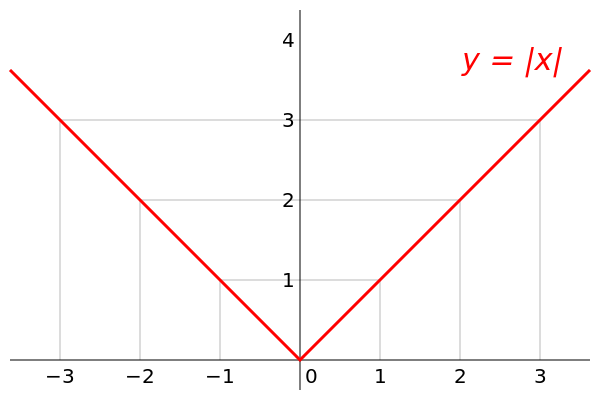
\includegraphics[height=5cm]{figures/Absolute_value_svg} 
\end{figure}


\noindent We hebben er toen ook op gewezen dat je voorzichtig moet
zijn met formules van het type $\sqrt{x^{2}}$.

\noindent Passen we dit toe op een functie die horizontaal verschoven
is: ${\displaystyle y=\sqrt{(x-1)^{2}}=\left|x-1\right|}$.

\noindent Als deze functie zou gegeven zijn als de veelterm ${\displaystyle x^{2}-2x+1}$,
dan loont het dus de moeite om dit te herschrijven als een volledig
kwadraat: ${\displaystyle x^{2}-2x+1=\left(x-1\right)^{2}}$.


\section{De signum functie}

De sign of signum functie $\textrm{sgn}(x)$ is een eenvoudige wiskundige
functie, die eigenlijk het teken van het argument aangeeft:

${\displaystyle \textrm{sgn}(x)=\begin{cases}
-1 & \textrm{als}\:x<0\\
0 & \textrm{\textrm{als}}\:x=0\\
+1 & \textrm{\textrm{als}}\:x>0
\end{cases}}$

\medskip{}


\noindent De grafiek van de signum functie:

\noindent 
\begin{figure}[h]
\centering{}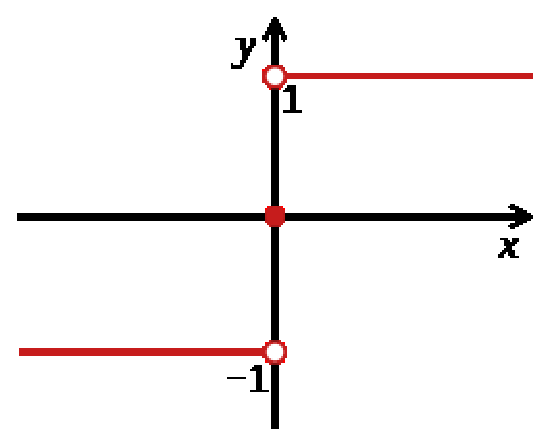
\includegraphics[height=5cm]{figures/Signum_function_svg} 
\end{figure}

\end{document}

%%\DeclareMathOperator{\tri}{tri} \DeclareMathOperator{\rect}{rect}
%\DeclareMathOperator{\sgn}{sgn} \DeclareMathOperator{\ramp}{ramp}
%\DeclareMathOperator{\sinc}{sinc}


\subsection{Verschuiven en herschalen}

%\begin{itemize}
%\item Wat gebeurt er met de grafiek van een functie als we bij het argument
%en/of bij de functie zelf, een getal optellen?
%\item Wat gebeurt er met de grafiek van een functie als we het argument
%en/of de functie zelf vermenigvuldigen met een getal?
%\end{itemize}

\subsubsection{Verschuiven}

Wanneer we de grafiek van $y=f(x)$ kennen, kunnen we met
verschuivingen (of translaties) de grafiek van $y=f(x+a)$ en $y=f(x)+a$
daaruit afleiden (met $a\in\mathbb{R}$).

De grafiek van $y=f(x+a)$ wordt verkregen uit de grafiek
van $y=f(x)$ door alle punten op de grafiek met een afstand van $a$
eenheden horizontaal te verschuiven (naar links als $a>0$, en naar
rechts als $a<0$).

Het lijkt misschien een beetje tegenstrijdig dat de grafiek
van een functie naar rechts verschuift als je bij het argument $x$
een negatief getal optelt. Maar kijk eens naar de sinus functie $f_{1}(x)=\sin(x)$
in onderstaand voorbeeld. We weten dat de sinus functie onder andere
een nulpunt heeft als het argument nul is, dus voor $x=0$. Als we
van $x$ de waarde $\frac{\pi}{2}$ aftrekken, dan bekomen we terug
datzelfde nulpunt als het argument nul is. Uit $x-\frac{\pi}{2}=0$
volgt dat dit het geval zal zijn als $x=+\frac{\pi}{2}$. Met andere
woorden, de functie $f_{2}(x)=\sin(x-\frac{\pi}{2})$ heeft dezelfde
grafiek als de functie $f_{1}(x)=\sin(x)$ maar is $\frac{\pi}{2}$
eenheden naar rechts verschoven.

%TODO figuur aanpassen
%\begin{figure}[h]
\begin{center}
	
%TODO polynoombenadering uitrekenen > zie cursus Algebra

\begin{tikzpicture}[scale=1,cap=round]

% Styles
\tikzstyle{axes}=[]
\tikzstyle help lines=[color=blue!50,very thin,dotted]


%%%%%%%%%%%%%%%%%%%%%%%%%%%%%%%%
%		GRID
%%%%%%%%%%%%%%%%%%%%%%%%%%%%%%%%

\draw[style=help lines,step=1cm] (-6.9,-3.9) grid (6.9,3.9);



%%%%%%%%%%%%%%%%%%%%%%%%%%%%%%%%
%		ASSENSTELSEL
%%%%%%%%%%%%%%%%%%%%%%%%%%%%%%%%

\draw[->] (-7,0) -- (7,0) node[right] {$x$};
\draw[->] (0,-4) -- (0,4) node[left]{$y$};

%\draw[fill,cyan](1,1)circle [radius=0.025];

%\draw[red,cap=rect, loosely dashed, ultra thick, domain=-2:2] plot (\x, {(\x*\x-1)+0.05}) node[above,yshift=-.7cm, right]{};

%%%%%%%%%%%%%%%%%%%%%%%%%%%%%%%%
%legende
%%%%%%%%%%%%%%%%%%%%%%%%%%%%%%%%
%\tkzDefPoint(0.5,3.5){A}
%\tkzDefPoint(1,3.5){B}
%\tkzLabelPoint[right,xshift=+0.1cm](B){${\color{cyan}f(x)=|x^2-1|}$}
%\tkzDrawSegment[cyan,ultra thick](A,B)

%\tkzDefPoint(0.5,3.2){C}
%\tkzDefPoint(1,3.2){D}
%\tkzLabelPoint[right,xshift=+0.1cm](D){${\color{red}e(x)=x^2-1}$}
%\tkzDrawSegment[red,cap=rect, loosely dashed, ultra thick](C,D)


%%%%%%%%%%%%%%%%%%%%%%%%%%%%%%%%
%getallen op de x-as en lijntjes
%%%%%%%%%%%%%%%%%%%%%%%%%%%%%%%%   
\foreach \x/\xtext in {-6,-5,-4,-3,-2,-1,1,2,3,4,5,6}
	\draw[xshift=\x cm] (0pt,1pt) -- (0pt,0pt) node[below,fill=white]
	{$\xtext$};,3
	
%getallen op de y-as en lijntjes  
%BEGIN LUS
\foreach \y/\ytext in {-3,-2,-1,1,2,3}
	\draw[yshift=\y cm] (1pt,0pt) -- (0pt,0pt) node[left,fill=white]
	{$\ytext$}; %EINDE LUS



%%%%%%%%%%%%%%%%%%%%%%%%%%%%%%%%
%		GRAFIEKEN
%%%%%%%%%%%%%%%%%%%%%%%%%%%%%%%%


\draw[teal,cap=rect,line width=2, opacity=0.8, domain=-7:7,samples=100] plot (\x, {
	sin(\x r)	% <- plaats het functievoorschrift hier	
}) node[opacity=1,,pos=0,xshift=+6cm,yshift=+1.5cm]{$f_1(x)=\sin{x}$};
%-------------------------------------------
\draw[red,cap=rect,line width=1, opacity=1, domain=-7:7,samples=100] plot (\x, {
	sin((\x +pi/2) r)	% <- plaats het functievoorschrift hier	
}) node[opacity=1,,pos=0,xshift=-6cm,yshift=+1.5cm]{$f_2(x)=\sin{x+\frac{\pi}{2}}$};
%-------------------------------------------



%\draw[cyan,cap=rect,thick, domain=-6:6] plot (\x, \x) node[above, right]{${\color{cyan}y=x}$};v

%\draw[cyan,cap=rect,ultra thick, domain=-6:1.75] plot (\x, {(\x-2)^(-1)}) node[above,right]{};


%\draw[cyan,cap=rect,ultra thick, domain=2.25:6] plot (\x, {(\x-2)^(-1)}) node[above,yshift=+0.5cm,left]{$\color{cyan} y=\frac{1}{x-2}$};


%\draw[cyan,cap=rect,ultra thick, domain=-7:1.9] plot (\x, {exp{\x}}) node[above, right]{${\color{cyan}y=\exp{x}}$};

%%%%%%%%%%%%%%%%%%%%%%%%%%%%%%%%
%		MARKERINGEN
%%%%%%%%%%%%%%%%%%%%%%%%%%%%%%%%
%verticale lijn
%\draw[-o,line width=4,teal, cap=rect,opacity=0.3] (0,-4) -- (0,0.25) node[right] {};
%\draw[line width=4,teal, cap=rect,opacity=0.3] (0,0) -- (0,4.2) node[right] {bld $f$ = $\mathbb{R}_0$};
%horizontale lijn
%\draw[arrows=-o,line width=4,blue, cap=rect,opacity=0.3] (-7,0) -- (2.25,0) node[right] {};
%\draw[line width=4,blue, cap=rect,opacity=0.3] (2.25,0) -- (7,0) node[below,yshift=-0.3cm] {dom$f$ = $\mathbb{R}  \setminus 2 $};
 
\end{tikzpicture}

\end{center}
%\end{figure}


\begin{center}
			\tikzsetfigurename{Fig_module_2_1_15_verschuiven_en_verschalen_2}



\begin{tikzpicture}[scale=1,cap=round]

% Styles
\tikzstyle{axes}=[]
\tikzstyle help lines=[color=blue!50,very thin,dotted]


%%%%%%%%%%%%%%%%%%%%%%%%%%%%%%%%
%		GRID
%%%%%%%%%%%%%%%%%%%%%%%%%%%%%%%%

\draw[style=help lines,step=1cm] (-6.9,-3.9) grid (6.9,3.9);



%%%%%%%%%%%%%%%%%%%%%%%%%%%%%%%%
%		ASSENSTELSEL
%%%%%%%%%%%%%%%%%%%%%%%%%%%%%%%%

\draw[->] (-7,0) -- (7,0) node[right] {$x$};
\draw[->] (0,-4) -- (0,4) node[left]{$y$};

%\draw[fill,cyan](1,1)circle [radius=0.025];

%\draw[red,cap=rect, loosely dashed, ultra thick, domain=-2:2] plot (\x, {(\x*\x-1)+0.05}) node[above,yshift=-.7cm, right]{};

%%%%%%%%%%%%%%%%%%%%%%%%%%%%%%%%
%legende
%%%%%%%%%%%%%%%%%%%%%%%%%%%%%%%%
%\tkzDefPoint(0.5,3.5){A}
%\tkzDefPoint(1,3.5){B}
%\tkzLabelPoint[right,xshift=+0.1cm](B){${\color{cyan}f(x)=|x^2-1|}$}
%\tkzDrawSegment[cyan,ultra thick](A,B)

%\tkzDefPoint(0.5,3.2){C}
%\tkzDefPoint(1,3.2){D}
%\tkzLabelPoint[right,xshift=+0.1cm](D){${\color{red}e(x)=x^2-1}$}
%\tkzDrawSegment[red,cap=rect, loosely dashed, ultra thick](C,D)


%%%%%%%%%%%%%%%%%%%%%%%%%%%%%%%%
%getallen op de x-as en lijntjes
%%%%%%%%%%%%%%%%%%%%%%%%%%%%%%%%   
\foreach \x/\xtext in {-6,-5,-4,-3,-2,-1,1,2,3,4,5,6}
	\draw[xshift=\x cm] (0pt,1pt) -- (0pt,0pt) node[below,fill=white]
	{$\xtext$};,3
	
%getallen op de y-as en lijntjes  
%BEGIN LUS
\foreach \y/\ytext in {-3,-2,-1,1,2,3}
	\draw[yshift=\y cm] (1pt,0pt) -- (0pt,0pt) node[left,fill=white]
	{$\ytext$}; %EINDE LUS



%%%%%%%%%%%%%%%%%%%%%%%%%%%%%%%%
%		GRAFIEKEN
%%%%%%%%%%%%%%%%%%%%%%%%%%%%%%%%


\draw[teal,cap=rect,line width=2, opacity=0.8, domain=-7:7,samples=100] plot (\x, {
	sin(\x r)	% <- plaats het functievoorschrift hier	
}) node[opacity=1,,pos=0,xshift=+6cm,yshift=+1.5cm]{$f_1(x)=\sin{x}$};
%-------------------------------------------
\draw[red,cap=rect,line width=1, opacity=1, domain=-7:7,samples=100] plot (\x, {
	sin((\x -pi/2) r)	% <- plaats het functievoorschrift hier	
}) node[opacity=1,,pos=0,xshift=-6cm,yshift=+1.5cm]{$f_2(x)=\sin{x-\frac{\pi}{2}}$};
%-------------------------------------------



%\draw[cyan,cap=rect,thick, domain=-6:6] plot (\x, \x) node[above, right]{${\color{cyan}y=x}$};v

%\draw[cyan,cap=rect,ultra thick, domain=-6:1.75] plot (\x, {(\x-2)^(-1)}) node[above,right]{};


%\draw[cyan,cap=rect,ultra thick, domain=2.25:6] plot (\x, {(\x-2)^(-1)}) node[above,yshift=+0.5cm,left]{$\color{cyan} y=\frac{1}{x-2}$};


%\draw[cyan,cap=rect,ultra thick, domain=-7:1.9] plot (\x, {exp{\x}}) node[above, right]{${\color{cyan}y=\exp{x}}$};

%%%%%%%%%%%%%%%%%%%%%%%%%%%%%%%%
%		MARKERINGEN
%%%%%%%%%%%%%%%%%%%%%%%%%%%%%%%%
%verticale lijn
%\draw[-o,line width=4,teal, cap=rect,opacity=0.3] (0,-4) -- (0,0.25) node[right] {};
%\draw[line width=4,teal, cap=rect,opacity=0.3] (0,0) -- (0,4.2) node[right] {bld $f$ = $\mathbb{R}_0$};
%horizontale lijn
%\draw[arrows=-o,line width=4,blue, cap=rect,opacity=0.3] (-7,0) -- (2.25,0) node[right] {};
%\draw[line width=4,blue, cap=rect,opacity=0.3] (2.25,0) -- (7,0) node[below,yshift=-0.3cm] {dom$f$ = $\mathbb{R}  \setminus 2 $};
 
\end{tikzpicture}

\end{center}


%\begin{figure}[h]
%	\centering
%	\begin{subfigure}{.48\linewidth}
%	\includegraphics[height=5cm]{\string"2_elem_rekenvaardigheden_B/inputs/Verschuiven - horizontaal - naar links\string".eps}
%	\end{subfigure}
%	\begin{subfigure}{.48\linewidth}
%	 \includegraphics[height=5cm]{\string"2_elem_rekenvaardigheden_B/inputs/Verschuiven - horizontaal - naar rechts\string".eps} 
%	\end{subfigure}
%\end{figure}

De grafiek van $y=f(x)+a$ wordt verkregen uit de grafiek
van $y=f(x)$ door alle punten op de grafiek met een afstand van $a$
eenheden verticaal te verschuiven (naar beneden als $a<0$, en naar
boven als $a>0$).

%TODO figuur aanpassen
\begin{center}
	
%TODO polynoombenadering uitrekenen > zie cursus Algebra

\begin{tikzpicture}[scale=1,cap=round]

% Styles
\tikzstyle{axes}=[]
\tikzstyle help lines=[color=blue!50,very thin,dotted]


%%%%%%%%%%%%%%%%%%%%%%%%%%%%%%%%
%		GRID
%%%%%%%%%%%%%%%%%%%%%%%%%%%%%%%%

\draw[style=help lines,step=1cm] (-6.9,-3.9) grid (6.9,3.9);



%%%%%%%%%%%%%%%%%%%%%%%%%%%%%%%%
%		ASSENSTELSEL
%%%%%%%%%%%%%%%%%%%%%%%%%%%%%%%%

\draw[->] (-7,0) -- (7,0) node[right] {$x$};
\draw[->] (0,-4) -- (0,4) node[left]{$y$};

%\draw[fill,cyan](1,1)circle [radius=0.025];

%\draw[red,cap=rect, loosely dashed, ultra thick, domain=-2:2] plot (\x, {(\x*\x-1)+0.05}) node[above,yshift=-.7cm, right]{};

%%%%%%%%%%%%%%%%%%%%%%%%%%%%%%%%
%legende
%%%%%%%%%%%%%%%%%%%%%%%%%%%%%%%%
%\tkzDefPoint(0.5,3.5){A}
%\tkzDefPoint(1,3.5){B}
%\tkzLabelPoint[right,xshift=+0.1cm](B){${\color{cyan}f(x)=|x^2-1|}$}
%\tkzDrawSegment[cyan,ultra thick](A,B)

%\tkzDefPoint(0.5,3.2){C}
%\tkzDefPoint(1,3.2){D}
%\tkzLabelPoint[right,xshift=+0.1cm](D){${\color{red}e(x)=x^2-1}$}
%\tkzDrawSegment[red,cap=rect, loosely dashed, ultra thick](C,D)


%%%%%%%%%%%%%%%%%%%%%%%%%%%%%%%%
%getallen op de x-as en lijntjes
%%%%%%%%%%%%%%%%%%%%%%%%%%%%%%%%   
\foreach \x/\xtext in {-6,-5,-4,-3,-2,-1,1,2,3,4,5,6}
	\draw[xshift=\x cm] (0pt,1pt) -- (0pt,0pt) node[below,fill=white]
	{$\xtext$};,3
	
%getallen op de y-as en lijntjes  
%BEGIN LUS
\foreach \y/\ytext in {-3,-2,-1,1,2,3}
	\draw[yshift=\y cm] (1pt,0pt) -- (0pt,0pt) node[left,fill=white]
	{$\ytext$}; %EINDE LUS



%%%%%%%%%%%%%%%%%%%%%%%%%%%%%%%%
%		GRAFIEKEN
%%%%%%%%%%%%%%%%%%%%%%%%%%%%%%%%


\draw[teal,cap=rect,line width=2, opacity=0.8, domain=-7:7,samples=100] plot (\x, {
	sin(\x r)	% <- plaats het functievoorschrift hier	
}) node[opacity=1,,pos=0,xshift=+6cm,yshift=+1.5cm]{$f_1(x)=\sin{x}$};
%-------------------------------------------
\draw[red,cap=rect,line width=1, opacity=1, domain=-7:7,samples=100] plot (\x, {
	(sin((\x r))-2	% <- plaats het functievoorschrift hier	
}) node[opacity=1,,pos=0,xshift=-6cm,yshift=-3cm]{$f_2(x)=\sin{x}-2$};
%-------------------------------------------



%\draw[cyan,cap=rect,thick, domain=-6:6] plot (\x, \x) node[above, right]{${\color{cyan}y=x}$};v

%\draw[cyan,cap=rect,ultra thick, domain=-6:1.75] plot (\x, {(\x-2)^(-1)}) node[above,right]{};


%\draw[cyan,cap=rect,ultra thick, domain=2.25:6] plot (\x, {(\x-2)^(-1)}) node[above,yshift=+0.5cm,left]{$\color{cyan} y=\frac{1}{x-2}$};


%\draw[cyan,cap=rect,ultra thick, domain=-7:1.9] plot (\x, {exp{\x}}) node[above, right]{${\color{cyan}y=\exp{x}}$};

%%%%%%%%%%%%%%%%%%%%%%%%%%%%%%%%
%		MARKERINGEN
%%%%%%%%%%%%%%%%%%%%%%%%%%%%%%%%
%verticale lijn
%\draw[-o,line width=4,teal, cap=rect,opacity=0.3] (0,-4) -- (0,0.25) node[right] {};
%\draw[line width=4,teal, cap=rect,opacity=0.3] (0,0) -- (0,4.2) node[right] {bld $f$ = $\mathbb{R}_0$};
%horizontale lijn
%\draw[arrows=-o,line width=4,blue, cap=rect,opacity=0.3] (-7,0) -- (2.25,0) node[right] {};
%\draw[line width=4,blue, cap=rect,opacity=0.3] (2.25,0) -- (7,0) node[below,yshift=-0.3cm] {dom$f$ = $\mathbb{R}  \setminus 2 $};
 
\end{tikzpicture}

\end{center}


\begin{center}
	
%TODO polynoombenadering uitrekenen > zie cursus Algebra

\begin{tikzpicture}[scale=1,cap=round]

% Styles
\tikzstyle{axes}=[]
\tikzstyle help lines=[color=blue!50,very thin,dotted]


%%%%%%%%%%%%%%%%%%%%%%%%%%%%%%%%
%		GRID
%%%%%%%%%%%%%%%%%%%%%%%%%%%%%%%%

\draw[style=help lines,step=1cm] (-6.9,-3.9) grid (6.9,3.9);



%%%%%%%%%%%%%%%%%%%%%%%%%%%%%%%%
%		ASSENSTELSEL
%%%%%%%%%%%%%%%%%%%%%%%%%%%%%%%%

\draw[->] (-7,0) -- (7,0) node[right] {$x$};
\draw[->] (0,-4) -- (0,4) node[left]{$y$};

%\draw[fill,cyan](1,1)circle [radius=0.025];

%\draw[red,cap=rect, loosely dashed, ultra thick, domain=-2:2] plot (\x, {(\x*\x-1)+0.05}) node[above,yshift=-.7cm, right]{};

%%%%%%%%%%%%%%%%%%%%%%%%%%%%%%%%
%legende
%%%%%%%%%%%%%%%%%%%%%%%%%%%%%%%%
%\tkzDefPoint(0.5,3.5){A}
%\tkzDefPoint(1,3.5){B}
%\tkzLabelPoint[right,xshift=+0.1cm](B){${\color{cyan}f(x)=|x^2-1|}$}
%\tkzDrawSegment[cyan,ultra thick](A,B)

%\tkzDefPoint(0.5,3.2){C}
%\tkzDefPoint(1,3.2){D}
%\tkzLabelPoint[right,xshift=+0.1cm](D){${\color{red}e(x)=x^2-1}$}
%\tkzDrawSegment[red,cap=rect, loosely dashed, ultra thick](C,D)


%%%%%%%%%%%%%%%%%%%%%%%%%%%%%%%%
%getallen op de x-as en lijntjes
%%%%%%%%%%%%%%%%%%%%%%%%%%%%%%%%   
\foreach \x/\xtext in {-6,-5,-4,-3,-2,-1,1,2,3,4,5,6}
	\draw[xshift=\x cm] (0pt,1pt) -- (0pt,0pt) node[below,fill=white]
	{$\xtext$};,3
	
%getallen op de y-as en lijntjes  
%BEGIN LUS
\foreach \y/\ytext in {-3,-2,-1,1,2,3}
	\draw[yshift=\y cm] (1pt,0pt) -- (0pt,0pt) node[left,fill=white]
	{$\ytext$}; %EINDE LUS



%%%%%%%%%%%%%%%%%%%%%%%%%%%%%%%%
%		GRAFIEKEN
%%%%%%%%%%%%%%%%%%%%%%%%%%%%%%%%


\draw[teal,cap=rect,line width=2, opacity=0.8, domain=-7:7,samples=100] plot (\x, {
	sin(\x r)	% <- plaats het functievoorschrift hier	
}) node[opacity=1,,pos=0,xshift=+6cm,yshift=-1.5cm]{$f_1(x)=\sin{x}$};
%-------------------------------------------
\draw[red,cap=rect,line width=1, opacity=1, domain=-7:7,samples=100] plot (\x, {
	(sin((\x r))+2	% <- plaats het functievoorschrift hier	
}) node[opacity=1,,pos=0,xshift=-6cm,yshift=+3.5cm]{$f_2(x)=\sin{x}+2$};
%-------------------------------------------



%\draw[cyan,cap=rect,thick, domain=-6:6] plot (\x, \x) node[above, right]{${\color{cyan}y=x}$};v

%\draw[cyan,cap=rect,ultra thick, domain=-6:1.75] plot (\x, {(\x-2)^(-1)}) node[above,right]{};


%\draw[cyan,cap=rect,ultra thick, domain=2.25:6] plot (\x, {(\x-2)^(-1)}) node[above,yshift=+0.5cm,left]{$\color{cyan} y=\frac{1}{x-2}$};


%\draw[cyan,cap=rect,ultra thick, domain=-7:1.9] plot (\x, {exp{\x}}) node[above, right]{${\color{cyan}y=\exp{x}}$};

%%%%%%%%%%%%%%%%%%%%%%%%%%%%%%%%
%		MARKERINGEN
%%%%%%%%%%%%%%%%%%%%%%%%%%%%%%%%
%verticale lijn
%\draw[-o,line width=4,teal, cap=rect,opacity=0.3] (0,-4) -- (0,0.25) node[right] {};
%\draw[line width=4,teal, cap=rect,opacity=0.3] (0,0) -- (0,4.2) node[right] {bld $f$ = $\mathbb{R}_0$};
%horizontale lijn
%\draw[arrows=-o,line width=4,blue, cap=rect,opacity=0.3] (-7,0) -- (2.25,0) node[right] {};
%\draw[line width=4,blue, cap=rect,opacity=0.3] (2.25,0) -- (7,0) node[below,yshift=-0.3cm] {dom$f$ = $\mathbb{R}  \setminus 2 $};
 
\end{tikzpicture}

\end{center}



%\begin{figure}[h]
%	\centering
%	\begin{subfigure}{.48\linewidth}
%		\includegraphics[height=5cm]{\string"2_elem_rekenvaardigheden_B/inputs/Verschuiven - verticaal - naar omlaag\string".eps}
%	\end{subfigure}
%	\begin{subfigure}{.48\linewidth}
%		\includegraphics[height=5cm]{\string"2_elem_rekenvaardigheden_B/inputs/Verschuiven - verticaal - naar o%mhoog\string".eps}
%	\end{subfigure}
%\end{figure}

%%\begin{tabular}{ccc}
%%\includegraphics[height=5cm]{\string"2_elem_rekenvaardigheden_B/inputs/Verschuiven - verticaal - naar omlaag\string".eps}  &  & \includegraphics[height=5cm]{\string"2_elem_rekenvaardigheden_B/inputs/Verschuiven - verticaal -  naar omhoog\string".eps} \tabularnewline
%%\end{tabular}


\begin{voorbeeld}
hoe ziet de grafiek eruit van de functie $y=x^{2}+2x+3$?

We herschrijven de functie als: $y=\left(x^{2}+2x+1\right)+2=\left(x+1\right)^{2}+2$

We herkennen hierin de basisfunctie $y=x^{2}$. De gegeven functie
stelt dus een parabool voor die over 1 eenheid naar links en 2 eenheden
naar boven is verschoven.
\end{voorbeeld}


\subsubsection{Herschalen}

Wanneer we de grafiek van $y=f(x)$ kennen, kunnen we met
herschalen (of vermenigvuldigen) de grafiek van $y=f(ax)$ en $y=af(x)$
daaruit afleiden (met $a\in\mathbb{R}$).

De grafiek van $y=f(ax)$ wordt verkregen uit de grafiek
van $y=f(x)$ door, bij gelijkblijvende $y$-co\"ordinaten, alle $x$-co\"ordinaten
van de punten op de grafiek met een factor $\frac{1}{a}$ te vermenigvuldigen
(openrekken als $0<a<1$, en inkrimpen als $a>1$).

Voor $a=2$ bijvoorbeeld krimpt de grafiek in elkaar. Het
is alsof de functie dubbel zo snel verloopt.

%TODO figuur aanpassen
\begin{center}
			\tikzsetfigurename{Fig_module_2_1_15_verschuiven_en_verschalen_5}


\begin{tikzpicture}[scale=1,cap=round]

% Styles
\tikzstyle{axes}=[]
\tikzstyle help lines=[color=blue!50,very thin,dotted]


%%%%%%%%%%%%%%%%%%%%%%%%%%%%%%%%
%		GRID
%%%%%%%%%%%%%%%%%%%%%%%%%%%%%%%%

\draw[style=help lines,step=1cm] (-6.9,-3.9) grid (6.9,3.9);



%%%%%%%%%%%%%%%%%%%%%%%%%%%%%%%%
%		ASSENSTELSEL
%%%%%%%%%%%%%%%%%%%%%%%%%%%%%%%%

\draw[->] (-7,0) -- (7,0) node[right] {$x$};
\draw[->] (0,-4) -- (0,4) node[left]{$y$};

%\draw[fill,cyan](1,1)circle [radius=0.025];

%\draw[red,cap=rect, loosely dashed, ultra thick, domain=-2:2] plot (\x, {(\x*\x-1)+0.05}) node[above,yshift=-.7cm, right]{};

%%%%%%%%%%%%%%%%%%%%%%%%%%%%%%%%
%legende
%%%%%%%%%%%%%%%%%%%%%%%%%%%%%%%%
%\tkzDefPoint(0.5,3.5){A}
%\tkzDefPoint(1,3.5){B}
%\tkzLabelPoint[right,xshift=+0.1cm](B){${\color{cyan}f(x)=|x^2-1|}$}
%\tkzDrawSegment[cyan,ultra thick](A,B)

%\tkzDefPoint(0.5,3.2){C}
%\tkzDefPoint(1,3.2){D}
%\tkzLabelPoint[right,xshift=+0.1cm](D){${\color{red}e(x)=x^2-1}$}
%\tkzDrawSegment[red,cap=rect, loosely dashed, ultra thick](C,D)


%%%%%%%%%%%%%%%%%%%%%%%%%%%%%%%%
%getallen op de x-as en lijntjes
%%%%%%%%%%%%%%%%%%%%%%%%%%%%%%%%   
\foreach \x/\xtext in {-6,-5,-4,-3,-2,-1,1,2,3,4,5,6}
	\draw[xshift=\x cm] (0pt,1pt) -- (0pt,0pt) node[below,fill=white]
	{$\xtext$};,3
	
%getallen op de y-as en lijntjes  
%BEGIN LUS
\foreach \y/\ytext in {-3,-2,-1,1,2,3}
	\draw[yshift=\y cm] (1pt,0pt) -- (0pt,0pt) node[left,fill=white]
	{$\ytext$}; %EINDE LUS



%%%%%%%%%%%%%%%%%%%%%%%%%%%%%%%%
%		GRAFIEKEN
%%%%%%%%%%%%%%%%%%%%%%%%%%%%%%%%


\draw[teal,cap=rect,line width=2, opacity=0.8, domain=-7:7,samples=100] plot (\x, {
	sin(\x r)	% <- plaats het functievoorschrift hier	
}) node[opacity=1,,pos=0,xshift=+6cm,yshift=-1.5cm]{$f_1(x)=\sin{x}$};
%-------------------------------------------
\draw[red,cap=rect,line width=1, opacity=1, domain=-7:7,samples=100] plot (\x, {
	(sin(0.5*(\x r))	% <- plaats het functievoorschrift hier	
}) node[opacity=1,,pos=0,xshift=-5cm,yshift=+1.5cm]{$f_2(x)=0.5\sin{x}+2$};
%-------------------------------------------



%\draw[cyan,cap=rect,thick, domain=-6:6] plot (\x, \x) node[above, right]{${\color{cyan}y=x}$};v

%\draw[cyan,cap=rect,ultra thick, domain=-6:1.75] plot (\x, {(\x-2)^(-1)}) node[above,right]{};


%\draw[cyan,cap=rect,ultra thick, domain=2.25:6] plot (\x, {(\x-2)^(-1)}) node[above,yshift=+0.5cm,left]{$\color{cyan} y=\frac{1}{x-2}$};


%\draw[cyan,cap=rect,ultra thick, domain=-7:1.9] plot (\x, {exp{\x}}) node[above, right]{${\color{cyan}y=\exp{x}}$};

%%%%%%%%%%%%%%%%%%%%%%%%%%%%%%%%
%		MARKERINGEN
%%%%%%%%%%%%%%%%%%%%%%%%%%%%%%%%
%verticale lijn
%\draw[-o,line width=4,teal, cap=rect,opacity=0.3] (0,-4) -- (0,0.25) node[right] {};
%\draw[line width=4,teal, cap=rect,opacity=0.3] (0,0) -- (0,4.2) node[right] {bld $f$ = $\mathbb{R}_0$};
%horizontale lijn
%\draw[arrows=-o,line width=4,blue, cap=rect,opacity=0.3] (-7,0) -- (2.25,0) node[right] {};
%\draw[line width=4,blue, cap=rect,opacity=0.3] (2.25,0) -- (7,0) node[below,yshift=-0.3cm] {dom$f$ = $\mathbb{R}  \setminus 2 $};
 
\end{tikzpicture}

\end{center}

\begin{center}
			\tikzsetfigurename{Fig_module_2_1_15_verschuiven_en_verschalen_6}


\begin{tikzpicture}[scale=1,cap=round]

% Styles
\tikzstyle{axes}=[]
\tikzstyle help lines=[color=blue!50,very thin,dotted]


%%%%%%%%%%%%%%%%%%%%%%%%%%%%%%%%
%		GRID
%%%%%%%%%%%%%%%%%%%%%%%%%%%%%%%%

\draw[style=help lines,step=1cm] (-6.9,-3.9) grid (6.9,3.9);



%%%%%%%%%%%%%%%%%%%%%%%%%%%%%%%%
%		ASSENSTELSEL
%%%%%%%%%%%%%%%%%%%%%%%%%%%%%%%%

\draw[->] (-7,0) -- (7,0) node[right] {$x$};
\draw[->] (0,-4) -- (0,4) node[left]{$y$};

%\draw[fill,cyan](1,1)circle [radius=0.025];

%\draw[red,cap=rect, loosely dashed, ultra thick, domain=-2:2] plot (\x, {(\x*\x-1)+0.05}) node[above,yshift=-.7cm, right]{};

%%%%%%%%%%%%%%%%%%%%%%%%%%%%%%%%
%legende
%%%%%%%%%%%%%%%%%%%%%%%%%%%%%%%%
%\tkzDefPoint(0.5,3.5){A}
%\tkzDefPoint(1,3.5){B}
%\tkzLabelPoint[right,xshift=+0.1cm](B){${\color{cyan}f(x)=|x^2-1|}$}
%\tkzDrawSegment[cyan,ultra thick](A,B)

%\tkzDefPoint(0.5,3.2){C}
%\tkzDefPoint(1,3.2){D}
%\tkzLabelPoint[right,xshift=+0.1cm](D){${\color{red}e(x)=x^2-1}$}
%\tkzDrawSegment[red,cap=rect, loosely dashed, ultra thick](C,D)


%%%%%%%%%%%%%%%%%%%%%%%%%%%%%%%%
%getallen op de x-as en lijntjes
%%%%%%%%%%%%%%%%%%%%%%%%%%%%%%%%   
\foreach \x/\xtext in {-6,-5,-4,-3,-2,-1,1,2,3,4,5,6}
	\draw[xshift=\x cm] (0pt,1pt) -- (0pt,0pt) node[below,fill=white]
	{$\xtext$};,3
	
%getallen op de y-as en lijntjes  
%BEGIN LUS
\foreach \y/\ytext in {-3,-2,-1,1,2,3}
	\draw[yshift=\y cm] (1pt,0pt) -- (0pt,0pt) node[left,fill=white]
	{$\ytext$}; %EINDE LUS



%%%%%%%%%%%%%%%%%%%%%%%%%%%%%%%%
%		GRAFIEKEN
%%%%%%%%%%%%%%%%%%%%%%%%%%%%%%%%


\draw[teal,cap=rect,line width=2, opacity=0.8, domain=-7:7,samples=100] plot (\x, {
	sin(\x r)	% <- plaats het functievoorschrift hier	
}) node[opacity=1,,pos=0,xshift=+6cm,yshift=-1.5cm]{$f_1(x)=\sin{x}$};
%-------------------------------------------
\draw[red,cap=rect,line width=1, opacity=1, domain=-7:7,samples=100] plot (\x, {
	(sin(2*(\x r))	% <- plaats het functievoorschrift hier	
}) node[opacity=1,,pos=0,xshift=-5.cm,yshift=+1.5cm]{$f_2(x)=0.3\sin{x}+2$};
%-------------------------------------------



%\draw[cyan,cap=rect,thick, domain=-6:6] plot (\x, \x) node[above, right]{${\color{cyan}y=x}$};v

%\draw[cyan,cap=rect,ultra thick, domain=-6:1.75] plot (\x, {(\x-2)^(-1)}) node[above,right]{};


%\draw[cyan,cap=rect,ultra thick, domain=2.25:6] plot (\x, {(\x-2)^(-1)}) node[above,yshift=+0.5cm,left]{$\color{cyan} y=\frac{1}{x-2}$};


%\draw[cyan,cap=rect,ultra thick, domain=-7:1.9] plot (\x, {exp{\x}}) node[above, right]{${\color{cyan}y=\exp{x}}$};

%%%%%%%%%%%%%%%%%%%%%%%%%%%%%%%%
%		MARKERINGEN
%%%%%%%%%%%%%%%%%%%%%%%%%%%%%%%%
%verticale lijn
%\draw[-o,line width=4,teal, cap=rect,opacity=0.3] (0,-4) -- (0,0.25) node[right] {};
%\draw[line width=4,teal, cap=rect,opacity=0.3] (0,0) -- (0,4.2) node[right] {bld $f$ = $\mathbb{R}_0$};
%horizontale lijn
%\draw[arrows=-o,line width=4,blue, cap=rect,opacity=0.3] (-7,0) -- (2.25,0) node[right] {};
%\draw[line width=4,blue, cap=rect,opacity=0.3] (2.25,0) -- (7,0) node[below,yshift=-0.3cm] {dom$f$ = $\mathbb{R}  \setminus 2 $};
 
\end{tikzpicture}

\end{center}




%\begin{figure}[h]
%\begin{subfigure}{.5\linewidth}
%\includegraphics[height=5cm]{\string"2_elem_rekenvaardigheden_B/inputs/Herschalen - horizontaal - openrekken\string".eps}
%\end{subfigure}
%\begin{subfigure}{.5\linewidth}
%\includegraphics[height=5cm]{\string"2_elem_rekenvaardigheden_B/inputs/Herschalen - horizontaal - inkrimpen\string".eps}
%\end{subfigure}	
%\end{figure}

Een bijzonder geval treedt op als $a=-1$: de grafiek van
$g(x)=f(-x)$ kan uit de grafiek van $f(x)$ worden verkregen door
van alle punten op de grafiek de $x$-co\"ordinaten met -1 te vermenigvuldigen,
dus door de grafiek van $f(x)$ te spiegelen ten opzichte van de $y$-as.
Op die manier kan je bijvoorbeeld heel eenvoudig afleiden dat de grafiek
van de functie $g(x)=\sqrt{-x}$ bestaat en het spiegelbeeld is van
$f(x)=\sqrt{x}$. Terwijl de functie $f(x)$ enkel gedefinieerd is
voor alle positieve re\"ele getallen, is de functie $g(x)$ dit enkel
voor alle negatieve re\"ele getallen.


De grafiek van $y=af(x)$ wordt verkregen uit de grafiek
van $y=f(x)$ door, bij gelijkblijvende $x$-co\"ordinaten, alle $y$-co\"ordinaten
van de punten op de grafiek met een factor $a$ te vermenigvuldigen
(inkrimpen als $0<a<1$, en openrekken als $a>1$).

%TODO figuur aanpassen
\begin{center}
	
%TODO polynoombenadering uitrekenen > zie cursus Algebra

\begin{tikzpicture}[scale=1,cap=round]

% Styles
\tikzstyle{axes}=[]
\tikzstyle help lines=[color=blue!50,very thin,dotted]


%%%%%%%%%%%%%%%%%%%%%%%%%%%%%%%%
%		GRID
%%%%%%%%%%%%%%%%%%%%%%%%%%%%%%%%

\draw[style=help lines,step=1cm] (-6.9,-3.9) grid (6.9,3.9);



%%%%%%%%%%%%%%%%%%%%%%%%%%%%%%%%
%		ASSENSTELSEL
%%%%%%%%%%%%%%%%%%%%%%%%%%%%%%%%

\draw[->] (-7,0) -- (7,0) node[right] {$x$};
\draw[->] (0,-4) -- (0,4) node[left]{$y$};

%\draw[fill,cyan](1,1)circle [radius=0.025];

%\draw[red,cap=rect, loosely dashed, ultra thick, domain=-2:2] plot (\x, {(\x*\x-1)+0.05}) node[above,yshift=-.7cm, right]{};

%%%%%%%%%%%%%%%%%%%%%%%%%%%%%%%%
%legende
%%%%%%%%%%%%%%%%%%%%%%%%%%%%%%%%
%\tkzDefPoint(0.5,3.5){A}
%\tkzDefPoint(1,3.5){B}
%\tkzLabelPoint[right,xshift=+0.1cm](B){${\color{cyan}f(x)=|x^2-1|}$}
%\tkzDrawSegment[cyan,ultra thick](A,B)

%\tkzDefPoint(0.5,3.2){C}
%\tkzDefPoint(1,3.2){D}
%\tkzLabelPoint[right,xshift=+0.1cm](D){${\color{red}e(x)=x^2-1}$}
%\tkzDrawSegment[red,cap=rect, loosely dashed, ultra thick](C,D)


%%%%%%%%%%%%%%%%%%%%%%%%%%%%%%%%
%getallen op de x-as en lijntjes
%%%%%%%%%%%%%%%%%%%%%%%%%%%%%%%%   
\foreach \x/\xtext in {-6,-5,-4,-3,-2,-1,1,2,3,4,5,6}
	\draw[xshift=\x cm] (0pt,1pt) -- (0pt,0pt) node[below,fill=white]
	{$\xtext$};,3
	
%getallen op de y-as en lijntjes  
%BEGIN LUS
\foreach \y/\ytext in {-3,-2,-1,1,2,3}
	\draw[yshift=\y cm] (1pt,0pt) -- (0pt,0pt) node[left,fill=white]
	{$\ytext$}; %EINDE LUS



%%%%%%%%%%%%%%%%%%%%%%%%%%%%%%%%
%		GRAFIEKEN
%%%%%%%%%%%%%%%%%%%%%%%%%%%%%%%%


\draw[teal,cap=rect,line width=2, opacity=0.8, domain=-7:7,samples=100] plot (\x, {
	sin(\x r)	% <- plaats het functievoorschrift hier	
}) node[opacity=1,,pos=0,xshift=+6cm,yshift=-1.5cm]{$f_1(x)=\sin{x}$};
%-------------------------------------------
\draw[red,cap=rect,line width=1, opacity=1, domain=-7:7,samples=100] plot (\x, {
	0.3*(sin((\x r))	% <- plaats het functievoorschrift hier	
}) node[opacity=1,,pos=0,xshift=-5cm,yshift=+1.5cm]{$f_2(x)=0.3\sin{x}+2$};
%-------------------------------------------



%\draw[cyan,cap=rect,thick, domain=-6:6] plot (\x, \x) node[above, right]{${\color{cyan}y=x}$};v

%\draw[cyan,cap=rect,ultra thick, domain=-6:1.75] plot (\x, {(\x-2)^(-1)}) node[above,right]{};


%\draw[cyan,cap=rect,ultra thick, domain=2.25:6] plot (\x, {(\x-2)^(-1)}) node[above,yshift=+0.5cm,left]{$\color{cyan} y=\frac{1}{x-2}$};


%\draw[cyan,cap=rect,ultra thick, domain=-7:1.9] plot (\x, {exp{\x}}) node[above, right]{${\color{cyan}y=\exp{x}}$};

%%%%%%%%%%%%%%%%%%%%%%%%%%%%%%%%
%		MARKERINGEN
%%%%%%%%%%%%%%%%%%%%%%%%%%%%%%%%
%verticale lijn
%\draw[-o,line width=4,teal, cap=rect,opacity=0.3] (0,-4) -- (0,0.25) node[right] {};
%\draw[line width=4,teal, cap=rect,opacity=0.3] (0,0) -- (0,4.2) node[right] {bld $f$ = $\mathbb{R}_0$};
%horizontale lijn
%\draw[arrows=-o,line width=4,blue, cap=rect,opacity=0.3] (-7,0) -- (2.25,0) node[right] {};
%\draw[line width=4,blue, cap=rect,opacity=0.3] (2.25,0) -- (7,0) node[below,yshift=-0.3cm] {dom$f$ = $\mathbb{R}  \setminus 2 $};
 
\end{tikzpicture}

\end{center}

\begin{center}
	
%TODO polynoombenadering uitrekenen > zie cursus Algebra

\begin{tikzpicture}[scale=1,cap=round]

% Styles
\tikzstyle{axes}=[]
\tikzstyle help lines=[color=blue!50,very thin,dotted]


%%%%%%%%%%%%%%%%%%%%%%%%%%%%%%%%
%		GRID
%%%%%%%%%%%%%%%%%%%%%%%%%%%%%%%%

\draw[style=help lines,step=1cm] (-6.9,-3.9) grid (6.9,3.9);



%%%%%%%%%%%%%%%%%%%%%%%%%%%%%%%%
%		ASSENSTELSEL
%%%%%%%%%%%%%%%%%%%%%%%%%%%%%%%%

\draw[->] (-7,0) -- (7,0) node[right] {$x$};
\draw[->] (0,-4) -- (0,4) node[left]{$y$};

%\draw[fill,cyan](1,1)circle [radius=0.025];

%\draw[red,cap=rect, loosely dashed, ultra thick, domain=-2:2] plot (\x, {(\x*\x-1)+0.05}) node[above,yshift=-.7cm, right]{};

%%%%%%%%%%%%%%%%%%%%%%%%%%%%%%%%
%legende
%%%%%%%%%%%%%%%%%%%%%%%%%%%%%%%%
%\tkzDefPoint(0.5,3.5){A}
%\tkzDefPoint(1,3.5){B}
%\tkzLabelPoint[right,xshift=+0.1cm](B){${\color{cyan}f(x)=|x^2-1|}$}
%\tkzDrawSegment[cyan,ultra thick](A,B)

%\tkzDefPoint(0.5,3.2){C}
%\tkzDefPoint(1,3.2){D}
%\tkzLabelPoint[right,xshift=+0.1cm](D){${\color{red}e(x)=x^2-1}$}
%\tkzDrawSegment[red,cap=rect, loosely dashed, ultra thick](C,D)


%%%%%%%%%%%%%%%%%%%%%%%%%%%%%%%%
%getallen op de x-as en lijntjes
%%%%%%%%%%%%%%%%%%%%%%%%%%%%%%%%   
\foreach \x/\xtext in {-6,-5,-4,-3,-2,-1,1,2,3,4,5,6}
	\draw[xshift=\x cm] (0pt,1pt) -- (0pt,0pt) node[below,fill=white]
	{$\xtext$};,3
	
%getallen op de y-as en lijntjes  
%BEGIN LUS
\foreach \y/\ytext in {-3,-2,-1,1,2,3}
	\draw[yshift=\y cm] (1pt,0pt) -- (0pt,0pt) node[left,fill=white]
	{$\ytext$}; %EINDE LUS



%%%%%%%%%%%%%%%%%%%%%%%%%%%%%%%%
%		GRAFIEKEN
%%%%%%%%%%%%%%%%%%%%%%%%%%%%%%%%


\draw[teal,cap=rect,line width=2, opacity=0.8, domain=-7:7,samples=100] plot (\x, {
	sin(\x r)	% <- plaats het functievoorschrift hier	
}) node[opacity=1,,pos=0,xshift=+6cm,yshift=-1.5cm]{$f_1(x)=\sin{x}$};
%-------------------------------------------
\draw[red,cap=rect,line width=1, opacity=1, domain=-7:7,samples=100] plot (\x, {
	3*(sin((\x r))	% <- plaats het functievoorschrift hier	
}) node[opacity=1,,pos=0,xshift=-5cm,yshift=+1.5cm]{$f_2(x)=3\sin{x}$};
%-------------------------------------------



%\draw[cyan,cap=rect,thick, domain=-6:6] plot (\x, \x) node[above, right]{${\color{cyan}y=x}$};v

%\draw[cyan,cap=rect,ultra thick, domain=-6:1.75] plot (\x, {(\x-2)^(-1)}) node[above,right]{};


%\draw[cyan,cap=rect,ultra thick, domain=2.25:6] plot (\x, {(\x-2)^(-1)}) node[above,yshift=+0.5cm,left]{$\color{cyan} y=\frac{1}{x-2}$};


%\draw[cyan,cap=rect,ultra thick, domain=-7:1.9] plot (\x, {exp{\x}}) node[above, right]{${\color{cyan}y=\exp{x}}$};

%%%%%%%%%%%%%%%%%%%%%%%%%%%%%%%%
%		MARKERINGEN
%%%%%%%%%%%%%%%%%%%%%%%%%%%%%%%%
%verticale lijn
%\draw[-o,line width=4,teal, cap=rect,opacity=0.3] (0,-4) -- (0,0.25) node[right] {};
%\draw[line width=4,teal, cap=rect,opacity=0.3] (0,0) -- (0,4.2) node[right] {bld $f$ = $\mathbb{R}_0$};
%horizontale lijn
%\draw[arrows=-o,line width=4,blue, cap=rect,opacity=0.3] (-7,0) -- (2.25,0) node[right] {};
%\draw[line width=4,blue, cap=rect,opacity=0.3] (2.25,0) -- (7,0) node[below,yshift=-0.3cm] {dom$f$ = $\mathbb{R}  \setminus 2 $};
 
\end{tikzpicture}

\end{center}




%\begin{figure}[h]
%	\begin{subfigure}{.5\linewidth}
%	\includegraphics[height=5cm]{\string"2_elem_rekenvaardigheden_B/inputs/Herschalen - verticaal - i%nkrimpen\string".eps}
%	\end{subfigure}
%	\begin{subfigure}{.5\linewidth}
%	\includegraphics[height=5cm]{\string"2_elem_rekenvaardigheden_B/inputs/Herschalen - verticaal - o%penrekken\string".eps}
%	\end{subfigure}	
%\end{figure}



%\DeclareMathOperator{\tri}{tri} \DeclareMathOperator{\rect}{rect}
%\DeclareMathOperator{\sgn}{sgn} \DeclareMathOperator{\ramp}{ramp}
%\DeclareMathOperator{\sinc}{sinc}


\subsection{Co\"ordinatenstelsels}

%\begin{itemize}
%\item Hoe kunnen we op een \'e\'enduidige manier elk punt in het vlak of de
%ruimte een plaats geven?
%\item Welke co\"ordinatenstelsels worden er vaak gebruikt?
%\end{itemize}
%Een co\"ordinatenstelsel is een wiskundige methode die wordt gebruikt
%om de ligging van een punt weer te geven.

\subsubsection{Cartesisch of rechthoekig co\"ordinatenstelsel}

De vergelijking $y=f(x)$ voegt aan iedere $x$-waarde \'e\'enduidig een
$y$-waarde toe. Met $x_{0}$ komt bijvoorbeeld $y_{0}$ overeen volgens
$y_{0}=f(x_{0})$. Het getallenpaar $(x_{0}\,,\,y_{0})$ kunnen we
als punt P in een rechthoekig of cartesisch co\"ordinatenstelsel tekenen.
De twee co\"ordinaat-assen staan loodrecht op elkaar, de horizontale
as noemen we de X-as en de verticale as de Y-as. Het snijpunt is de
oorsprong O.

\noindent Voor ieder getallenpaar krijgen we precies \'e\'en punt. De
verzameling van alle punten $(x\,,\,y=f(x))$ vormt de grafiek of
kromme van de functie. De grafiek laat het verloop van de functie
in een figuur zien.

\begin{figure}
\centering
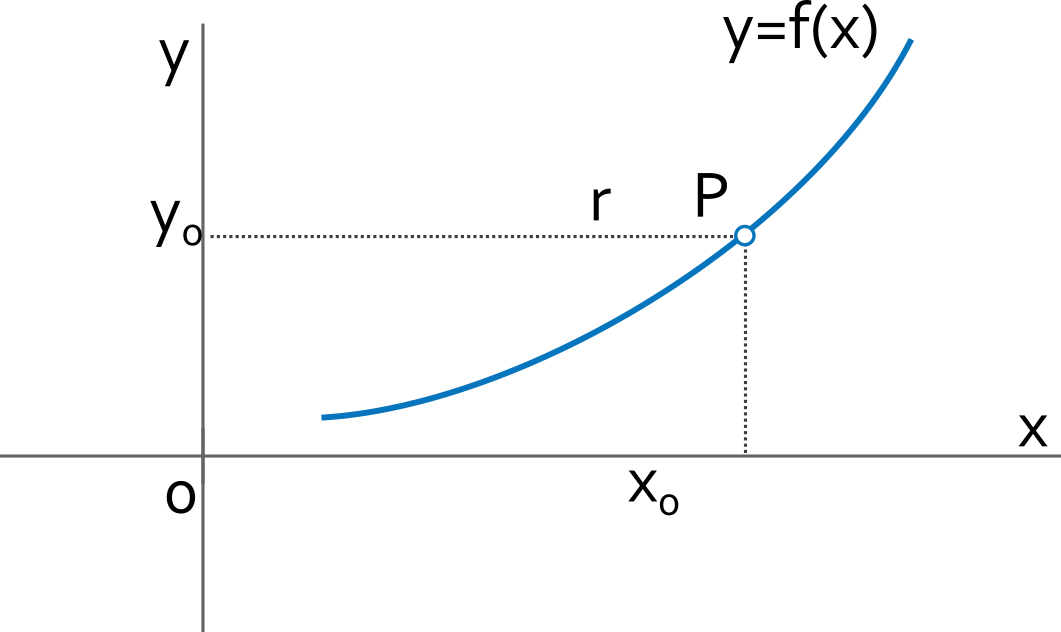
\includegraphics[height=5cm]{2_elem_rekenvaardigheden_B/inputs/figuur10}
\end{figure}

\begin{table}
	\centering
\begin{tabular}{|c|l|l|}
	\hline 
	We zeggen dat: & $x_{0},y_{0}$  & zijn de rechthoekige of cartesische co\"ordinaten\\
	\hline 
	& $x_{0}$  & is de abscis van het punt P\\
	\hline 
	& $y_{0}$ & is de ordinaat van het punt P\\
	\hline 
\end{tabular}
\end{table}


\noindent Het cartesisch co\"ordinatenstelsel is de gebruikelijke manier
om een punt in een vlak aan te duiden. Omdat in dit platte vlak twee
co\"ordinaten nodig zijn om een punt vast te leggen, zeggen we dat een
vlak tweedimensionaal is. In feite is 'de dimensie van een ruimte'
het aantal co\"ordinaten dat nodig is om de plaats van alle punten in
die ruimte precies te kunnen bepalen. Zo bestaat de klassieke 3D-ruimte
uit 3 dimensies en zijn er dus 3 co\"ordinaten $(x,y,z)$ nodig om de
plaats van elk punt \'e\'enduidig te beschrijven. 

\textbf{Parametervoorstelling van een functie}

\noindent Het is bij de wiskundige beschrijving van een bewegend lichaam
vaak handig om de positie van het lichaam weer te geven door cartesische
co\"ordinaten die zelf een functie van de tijd zijn. We noteren dan:
\[
x=x(t)\:,\;y=y(t)\quad\textrm{met}\:t_{1}\leq t\leq t_{2}
\]

\noindent We noemen een dergelijke voorstelling met een hulpvariabele
$t$ de parametervoorstelling van een functie. In de natuurwetenschappen
en de techniek betekent de parameter $t$ meestal de tijd of een hoek.

\noindent We krijgen voor iedere waarde van t uit het interval $t_{1}\leq t\leq t_{2}$
precies \'e\'en punt van de kromme.\medskip{}


\noindent Voorbeeld 1: de horizontale worp

\noindent een lichaam wordt van een bepaalde hoogte horizontaal met
een constante beginsnelheid $v_{0}$ weggeworpen. T.g.v. de zwaartekracht
verloopt de beweging vervolgens als een parabool (parabolische baan).
De parametervergelijkingen van deze beweging zijn:

\[
x=v_{0}t\:,\;y=\frac{1}{2}gt^{2}\quad\textrm{met}\:t\geq0
\]


\noindent Door het elimineren van de parameter vinden we de expliciete
vergelijking van de grafiek (parabool). Dit doen we door t uit de
vergelijking van $x$ te halen en te substitueren in de vergelijking
van $y$:

uit $x=v_{0}t$ volgt dat $t=\frac{x}{v_{0}}$ zodat $y=\frac{1}{2}gt^{2}=\frac{1}{2}g\left(\frac{x}{v_{0}}\right)^{2}=\frac{g}{2v_{0}^{2}}x$


\noindent Voorbeeld 2: de cirkel

Een veel gebruikte parametrisatie voor de cirkel met vergelijking
$x^{2}+y^{2}=R^{2}$ is de volgende:

\noindent 
\[
x=R\cos(t)\:,\;y=R\sin(t)\quad\textrm{met}\:0\leq t<2\pi
\]


Opmerkingen:
\begin{itemize}
\item de parameter $t$ stelt nu een hoek voor (uitgedrukt in radialen).
Omdat $t=0$ en $t=2\pi$ hetzelfde punt voorstellen, zal men meestal
$2\pi$ niet opnemen in het interval. Vandaar het $<$ en niet nog
eens het $\leq$-symbool.
\item om uit de parametervergelijkingen de cartesische vergelijking voor
de cirkel te bekomen moeten we de parameter t elimineren. Daarvoor
gebruiken we een trucje. We weten dat voor elke hoek $\alpha$ de
goniometrische grondformule geldt: $\cos^{2}\alpha+\sin^{2}\alpha=1$.
Substitueren we nu $\cos(t)=\frac{x}{R}$ en $\sin(t)=\frac{y}{R}$
in de grondformule dan bekomen we inderdaad $x^{2}+y^{2}=R^{2}$ .
\end{itemize}

\subsubsection{Poolco\"ordinaten}

De poolco\"ordinaten $\left(r,\theta\right)$ van een punt P in een
vlak zijn de afstandsco\"ordinaat $r$ en de hoekco\"ordinaat $\theta$.
We noemen de afstand $r$ de radius of de voerstraal en de hoek $\theta$
het argument.

\begin{figure}
\centering
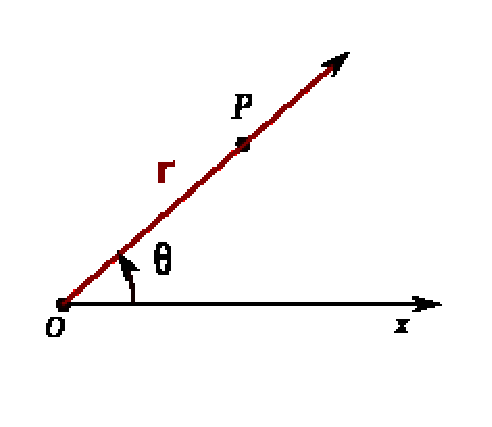
\includegraphics{2_elem_rekenvaardigheden_B/inputs/Poolcoordinaten_wikipedia}
\end{figure}

Enkele opmerkingen:
\begin{itemize}
\item we defini\"eren de voerstraal $r$ steeds positief, dus $r\geq0$.
\item we defini\"eren de hoek $\theta$ positief als de pijl van de positieve
X-as naar de plaatsvector van P tegen de klok in draait (andersom
is de hoek negatief). Een hoek $\theta$ is \'e\'enduidig bepaald op veelvouden
van 360\textdegree{} (of veelvouden van $2\pi$ in radialen) na. Meestal
wordt de hoek $\theta$ gegeven in het interval $0\text{\textdegree}\leq\theta\leq360\text{\textdegree}$
of $0\leq\theta\leq2\pi$. I.p.v. de Griekse letter theta ($\theta$
) wordt ook vaak de letter phi ( $\varphi$ ) als hoekaanduiding gebruikt.
\item de X- en Y-as maken geen deel uit van dit co\"ordinatenstelsel. We tekenen
echter wel vaak een horizontale en verticale hulplijn om het uitzetten
van de hoeken te vergemakkelijken.
\item het poolco\"ordinatenstelsel is een kromlijnig co\"ordinatenstelsel: de
co\"ordinaatlijnen zijn concentrische cirkels met de oorsprong O als
middelpunt en langs stralen die radiaal vanuit O lopen. We noemen
de oorsprong ook vaak 'de pool' en de X-as de 'poolas'.
\item de pool (dus de oorsprong O) heeft als voerstraal $r=0$ terwijl de
hoek $\theta$ onbepaald is.
\item poolco\"ordinaten worden ook gebruikt bij het voorstellen van en het
werken met complexe getallen.
\end{itemize}


\noindent Soms is het handig of noodzakelijk om over te stappen van
cartesische co\"ordinaten naar poolco\"ordinaten of omgekeerd. Daarvoor
gebruiken we het volgende stel transformatievergelijkingen:

\begin{minipage}{.48\linewidth}
%\begin{table}
	\begin{tabular}{|l|c|l|}
		\hline 
		cartesische co\"ordinaten &  & poolco\"ordinaten  \\
		\hline
		gegeven P met $\left(x,y\right)$ & $\rightarrow$ & dan is $\begin{cases}
		r=\sqrt{x^{2}+y^{2}}\\
		\textrm{tg}\theta=\frac{y}{x}
		\end{cases}$  \\
		dan is $\begin{cases}
		x=r.\cos\theta\\
		y=r.\sin\theta
		\end{cases}$ & $\leftarrow$ & gegeven P met $\left(r,\theta\right)$ \\
		\hline 
	\end{tabular}
%\end{table}
\end{minipage}
\hspace{1cm}
\begin{minipage}{.48\linewidth}
	\centering
	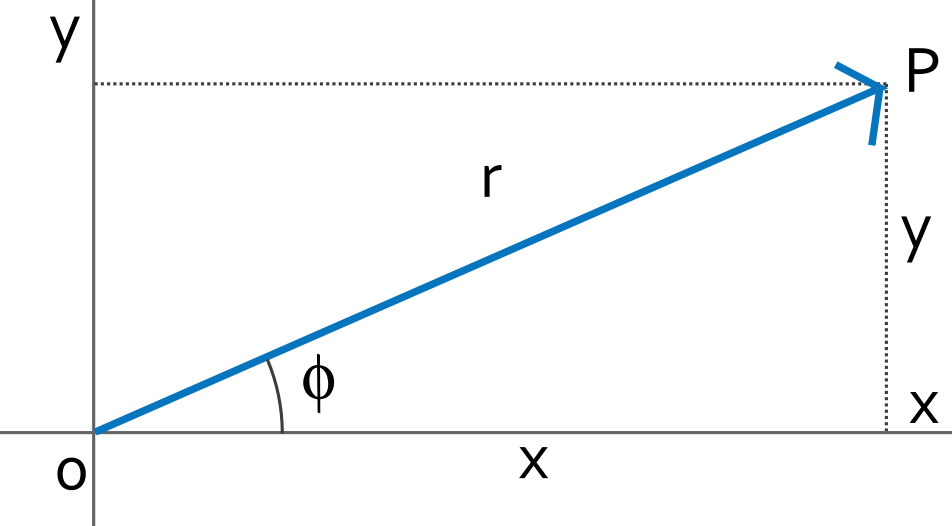
\includegraphics[width=0.7\linewidth]{2_elem_rekenvaardigheden_B/inputs/figuur9}
\end{minipage}


Opmerking: let op bij het berekenen van de hoek $\theta$. Je rekenmachine
zal als resultaat van de $\textrm{Arctg}\left(\frac{y}{x}\right)$
een hoek geven in het 1ste of 4de kwadrant. Je moet dus zelf, bij
het resultaat van je rekenmachine nog 180\textdegree{} of $\pi$ optellen
als het punt P in het 2de of 3de kwadrant ligt.

\noindent De voorstelling van een functie in poolco\"ordinaten

\noindent Een functie (kromme) in poolco\"ordinaten wordt beschreven
door een vergelijking van de vorm:
\[
r=r(\theta)
\]


\noindent We stellen een functiewaardentabel op voordat we de grafiek
van de functie tekenen. Voor verschillende waarden $\theta_{1}$ ,
$\theta_{2}$ , $\theta_{3}$ , ... berekenen we de bijhorende voerstralen
$r_{1}=r\left(\theta_{1}\right)$ , ... Daarna tekenen we de punten
met co\"ordinaten $\left(r_{1},\theta_{1}\right)$ , ... en verbinden
deze d.m.v. een vloeiende lijn.

\begin{minipage}{.48\linewidth}
	\centering
	\begin{tabular}{|c|c|}
		\hline 
		$\theta$ & $r=r(\theta)$\\
		\hline 
		\hline 
		$\theta_{1}$ & $r_{1}=r\left(\theta_{1}\right)$ \\
		\hline 
		$\theta_{2}$ & $r_{2}=r\left(\theta_{2}\right)$ \\
		\hline 
		$\vdots$ & $\vdots$\\
		\hline 
	\end{tabular}
\end{minipage}
\begin{minipage}{.48\linewidth}
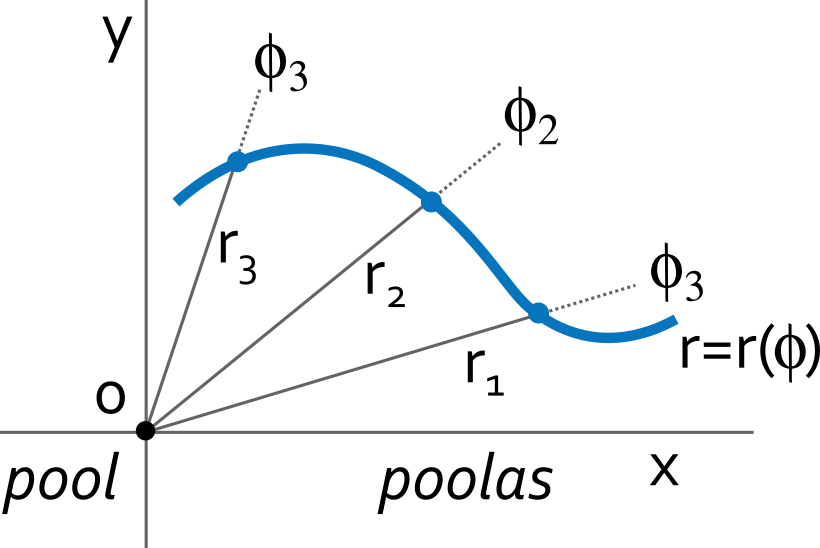
\includegraphics[height=5cm]{2_elem_rekenvaardigheden_B/inputs/figuur11}\\
In de figuur zijn de hoeken aangeduid met $\varphi$ ipv $\theta$
\end{minipage}



Voorbeeld 1: de spiraal van Archimedes

Schets de kromme met vergelijking $r=\theta$ waarbij $0\leq\theta\leq2\pi$

We stellen een functiewaardentabel op (tip: kies niet te veel, maar
ook niet te weinig hoeken; de intervallen tussen de hoeken hoeft niet
noodzakelijk overal even groot te zijn).

\begin{minipage}{.48\linewidth}
	\centering
	\begin{tabular}{|c|c|}
		\hline 
		$\theta$ & $r=r(\theta)=\theta$\\
		\hline 
		\hline 
		$0$ & 0\\
		\hline 
		$\frac{\pi}{4}$ & 0.785 \\
		\hline 
		$\frac{\pi}{2}$ & 1.571\\
		\hline 
		$3\frac{\pi}{4}$ & 2.356\\
		\hline 
		$\pi$ & 3.142\\
		\hline 
		$3\frac{\pi}{2}$ & 4.712\\
		\hline 
		$2\pi$ & 6.283\\
		\hline 
	\end{tabular}
\end{minipage}
\begin{minipage}{.48\linewidth}
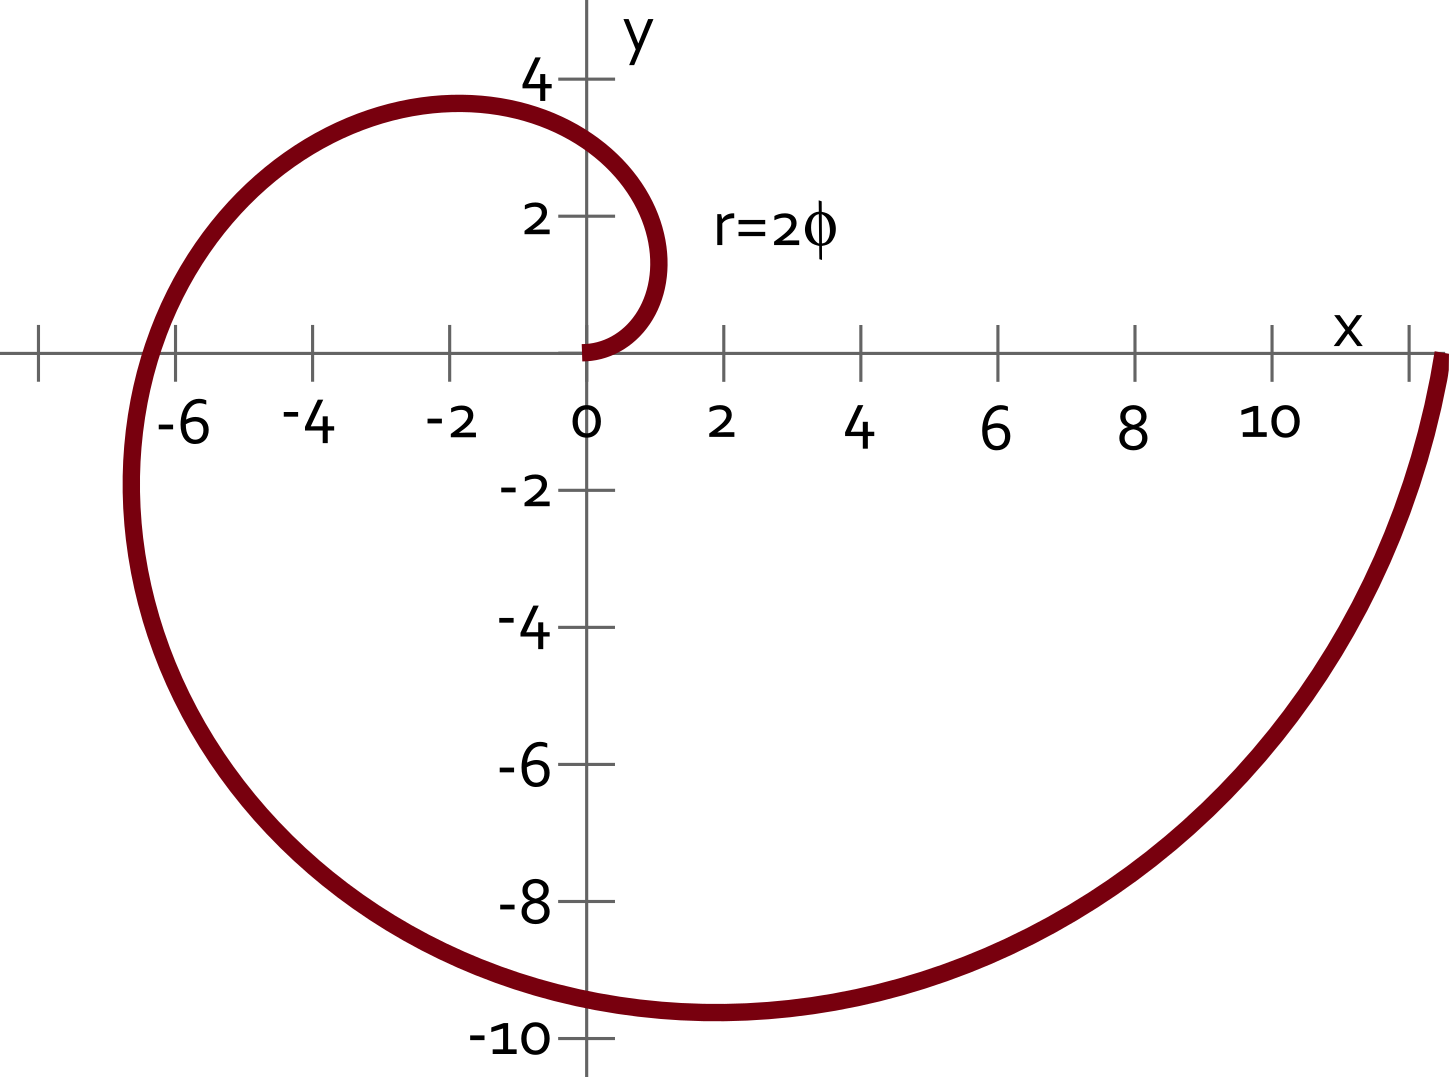
\includegraphics[height=5cm]{2_elem_rekenvaardigheden_B/inputs/figuur8}
\end{minipage}

Voorbeeld 2: de cardio\"ide

Schets de kromme met vergelijking $r=1+\cos\theta$ waarbij $0\text{\textdegree}\leq\theta\leq360\text{\textdegree}$

We stellen een functiewaardentabel op. Wegens de symmetrie t.o.v.
de X-as berekenen we slechts de radius-waarden tussen 0\textdegree{}
en 180\textdegree .

\begin{minipage}{0.5\linewidth}
	\centering
\begin{tabular}{|c|c|}
\hline 
$\theta$ & $r=r(\theta)$\\
\hline 
\hline 
0\textdegree{} & 2\\
\hline 
30\textdegree{} & 1.866\\
\hline 
60\textdegree{} & 1.5\\
\hline 
90\textdegree{} & 1\\
\hline 
120\textdegree{} & 0.5\\
\hline 
150\textdegree{} & 0.134\\
\hline 
180\textdegree{} & 0\\
\hline 
\end{tabular}
\end{minipage}
\begin{minipage}{.48\linewidth}
%	\begin{figure}
	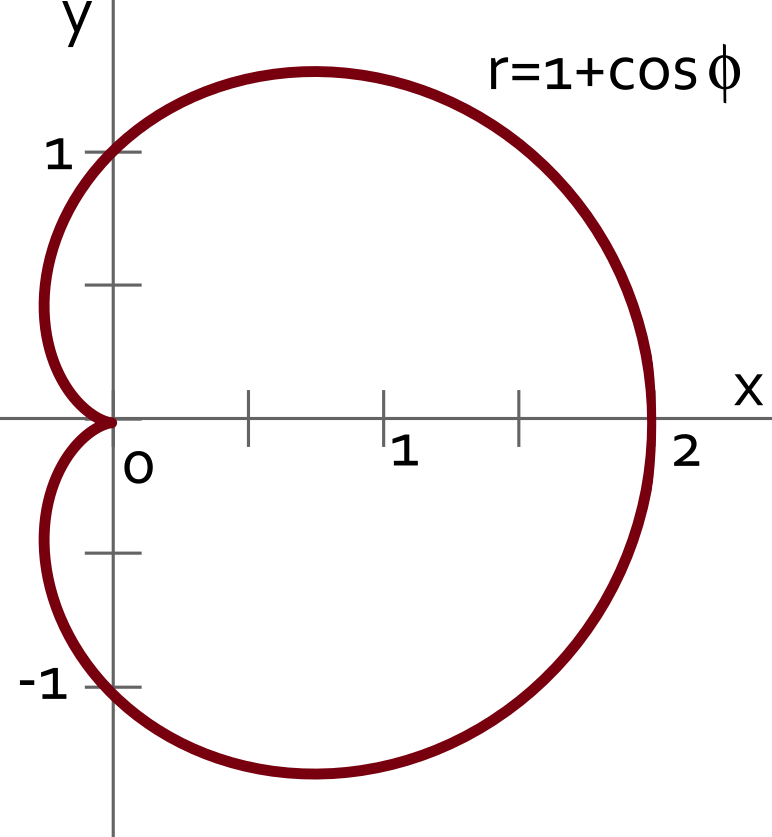
\includegraphics[height=5cm]{2_elem_rekenvaardigheden_B/inputs/figuur7.png}
%	\end{figure}
\end{minipage} 

Voorbeeld 3: de cirkel

Schets de kromme met vergelijking $r=2$ waarbij $0\text{\textdegree}\leq\theta<360\text{\textdegree}$

Bij elke hoek $\theta$ hoort dezelfde voerstraal, namelijk $r=2$.
Het heeft dus weinig zin om een functiewaardentabel op te stellen.

Opmerking: de cartesische vergelijking van een cirkel heeft een duidelijk
ingewikkeldere notatie: $x^{2}+y^{2}=2^{2}$. Schrijven we $y$ expliciet
dan zien we meteen ook dat dit eigenlijk geen functie is (met elke
$x$-waarde komen immers 2 $y$-waarden overeen): $y=\pm\sqrt{4-x^{2}}$



\pagebreak

\section{Limieten}

\subsection{Het begrip limiet}

Bij het bestuderen van het gedrag van een functie stuiten we soms
op het probleem dat de functie in een bepaald punt niet gedefini\"eerd
is. Dit kan bijvoorbeeld optreden als het voorschrift van de functie
een breuk is waarvan de noemer nul wordt in dat punt. Toch willen
we vaak weten hoe de grafiek van die functie in de buurt van zo'n
punt er uitziet. Ook zijn we ge\"interesseerd in het gedrag van een
functie als het argument zeer groot of zeer sterk negatieve waarden
aanneemt.

Het begrip limiet is dus een belangrijke bouwsteen van de
analyse. De begrippen continu\"iteit, onbepaalde integraal en bepaalde
integraal steunen allen op het limietbegrip. Ook meetkundig is het
limietbegrip van belang: men heeft het nodig bij de definitie van
afgeleiden en asymptoten.


\subsubsection{De verzameling $\bar{\mathbb{R}}$}

Gegeven is de verzameling van de re\"ele getallen $\mathbb{R}$. Stel,
we nemen als deelverzameling het halfopen interval $[5,10[$ van $\mathbb{R}$.
Er bestaat dan bijvoorbeeld een getal uit die verzameling dat kleiner
of gelijk is aan alle elementen uit die deelverzameling. We noteren
dit als $\forall x\in[5,10[$ waarvoor geldt dat $x\ge5$. In dit
geval is het gezochte getal 5. Maar dit is niet altijd zo eenvoudig.




Nemen we de deelverzameling $\{...3,5,7,9\}$ van $\mathbb{R}$.
Welk getal kunnen we vinden dat kleiner is dan alle elementen uit
deze deelverzameling? Het getal 1? Of -1? Of -100? Het antwoord wordt
gevonden door de verzameling uit te breiden met de elementen plus
oneindig ($+\infty$) en min oneindig ($-\infty$).




We zeggen nu dat ``streep R streep'' gelijk is aan: $\overline{\mathbb{R}}=\mathbb{R}\cup\{\text{\textminus\ensuremath{\infty}},+\text{\ensuremath{\infty}}\}$
waarbij $\forall x\in\mathbb{R}$ geldt dat $\text{\textminus\ensuremath{\infty}}<x<+\text{\ensuremath{\infty}}$.




Merk op dat de elementen $\text{\textminus\ensuremath{\infty}}$
en $+\text{\ensuremath{\infty}}$ zelf geen re\"ele getallen zijn. Let
ook op met het symbool $\infty$: afhankelijk van de context kan dit
\textquotedblleft$+\infty$\textquotedblright betekenen, maar ook \textquotedblleft$+\infty\:\mathrm{of}\:\text{\textminus\ensuremath{\infty}}$\textquotedblright.
In dit laatste geval schrijven we soms $\pm\infty$.


\subsubsection{Rekenen met $\infty$}

Alhoewel $\text{\textminus\ensuremath{\infty}}$ en $+\text{\ensuremath{\infty}}$
geen re\"ele getallen zijn (maar wel symbolen), kunnen we er toch (mits
enige voorzichtigheid) mee rekenen.



\begin{tabel*}{}
	\centering
	\begin{tabular}{lcc|ll}
		\multicolumn{3}{c|}{vermenigvuldiging} & \multicolumn{2}{c}{optelling}\\
		\hline 
		$a\cdot (+\infty)=+\infty$ & als & $a>0$ & $\pm\infty+a=\pm\infty$ & met $a\in\mathbb{R}$\\
		$a\cdot (+\infty)=-\infty$ & als & $a<0$ &  & \\
		$a\cdot (-\infty)=-\infty$ & als & $a>0$ &  & \\
		$a\cdot (-\infty)=+\infty$ & als & $a<0$ &  & \\
		&  &  &  & \\
		$(+\infty)\cdot (+\infty)=+\infty$ &  &   & $(+\infty)+(+\infty)=+\infty$ & \\
		$(-\infty)\cdot (-\infty)=+\infty$ &  &   & $(-\infty)+(-\infty)=-\infty$ & \\
		$(+\infty)\cdot (-\infty)=-\infty$ &  &   &  & \\
	\end{tabular}
\end{tabel*}




$\frac{1}{\infty}=0$ maar let op: $\frac{1}{0}=\infty$
en dus onbepaald (want $\infty$ is geen re\"eel getal).

Soms maken we nog onderscheid tussen een heel klein positief
of heel klein negatief getal: $\frac{1}{0^{+}}=+\infty$ en $\frac{1}{0^{-}}=-\infty$




De volgende vormen zijn ook onbepaald: $\frac{0}{0}$ en
$\frac{\infty}{\infty}$ , $0\cdot \infty$, $+\infty-\infty$ , $0{}^{0}$
, $\infty{}^{0}$ , $1{}^{\infty}$.

Hoezo, $1{}^{\infty}$ is onbepaald? Dit is toch gewoon
$1\cdot 1\cdot 1\cdot 1\cdot \,\ldots$ en dus gelijk aan $1$!? Het antwoord hierop vind
je op het einde van dit hoofdstukje.

Merk op dat de vormen $\frac{0}{0}$ en $\frac{\infty}{\infty}$
infeite hetzelfde betekenen, immers $\frac{a}{b}$ kan je ook schrijven
als $\frac{\frac{1}{b}}{\frac{1}{a}}$.

\subsection{Intu\"itieve uitleg limieten}
\begin{minipage}{.25\linewidth}
	\raggedright
	
\includegraphics[width=4cm]{2_elem_rekenvaardigheden_B/inputs/QR_Code_LIMIETEN_module2new}
\end{minipage}
\begin{minipage}{.7\linewidth}
	Zie filmpje MOOC.
\end{minipage}

\subsection{Limieten en continu\"iteit}

\subsubsection{Het limietbegrip}

Als $x$ nadert tot $a$, dan nadert $f(x)$ tot $b$.

We zeggen wiskundig: de limiet van $f(x)$ voor $x$ gaande
naar $a$ is $b$.

We noteren dit als: $\lim_{x\to a}f(x)=b$

Grafisch:


\begin{figure}[H]
\centering
\tikzsetfigurename{Fig_module_2_2_1_limietbegripvb1}

\begin{center}
\begin{tikzpicture}[scale=0.7,cap=round]

% Styles
\tikzstyle{axes}=[]
\tikzstyle help lines=[color=blue!50,very thin,dotted]

% grid
\draw[style=help lines,step=1cm] (-0.9,-0.9) grid (6.9,8.9);

\draw[->] (-1,0) -- (7,0) node[right] {$x$};
\draw[->] (0,-1) -- (0,9) node[above] {$y$};

%\draw[fill,cyan](1,1)circle [radius=0.025];
%FUNCTIEVOORSCHRIFTEN



%\draw[teal,cap=rect,line width=1, opacity=1, domain=-2:2] plot (\x, {
%	pow(\x,2)  		% <- plaats het functievoorschrift hier
%}) node[right,opacity=1]{$h(x)=x^2$};

%\draw[red,cap=rect,line width=1, opacity=1, domain=-1.5:1.5] plot (\x, {
%	pow(\x,4)  		% <- plaats het functievoorschrift hier
%}) node[opacity=1,above,xshift=-3.5cm]{$p(x)=x^4$};

\draw[blue,cap=rect,line width=1, opacity=1, domain=3:6] plot (\x, {
	pow(\x-4,3)+1	% <- plaats het functievoorschrift hier
}) node[opacity=1,xshift=+1cm]{};

\draw[-,red] (0,3.3)--(5.3,3.3); 
\draw[-,red] (5.3,0)--(5.3,3.3); 

\draw[-,gray] (0,1.6)--(4.8,1.6); 
\draw[-,gray] (4.8,0)--(4.8,1.6); 

\draw[-,gray] (0,7.3)--(5.8,7.3); 
\draw[-,gray] (5.8,0)--(5.8,7.3); 


\draw[red] (5.3,3.3) circle[radius=0.1];

\draw[] (5.3,-0.2) node[below,red] {$a$};

\draw[] (-0.2,3.3) node[left,red] {$f(a)$};


\draw[] (4.8,1.6) circle[radius=0.1];



\draw[] (4.8,-0.2) node[below] {$x$};
\draw[] (-0.2,1.6) node[left] {$f(x)$};



\draw[] (5.8,7.3) circle[radius=0.1];

\draw[] (5.8,-0.2) node[below] {$x$};
\draw[] (-0.2,7.3) node[left] {$f(x)$};

%\draw[orange,cap=rect,line width=1, opacity=1, domain=-1.4:1.4] plot (\x, {
%	pow(\x,5)  		% <- plaats het functievoorschrift hier
%}) node[right,opacity=1]{$g(x)=x^5$};



%\draw[cyan,cap=rect,ultra thick, domain=1:2] plot (\x, {\x*\x-1}) node[above, right]{};
%\draw[red,cap=rect, loosely dashed, ultra thick, domain=-2:2] plot (\x, {(\x*\x-1)+0.05}) node[above,yshift=-.7cm, right]{};

%legende



%getallen op de x-as en lijntjes   
%\foreach \x/\xtext in {0,2,4,6}
%	\draw[xshift=\x cm] (0pt,1pt) -- (0pt,0pt) node[below,fill=white]
%	{$\xtext$}; 
	
%getallen op de y-as en lijntjes  
%BEGIN LUS
%\foreach \y/\ytext in {2,4,6,8}
%	\draw[yshift=\y cm] (1pt,0pt) -- (0pt,0pt) node[left,fill=white]
%	{$\ytext$}; %EINDE LUS



\end{tikzpicture}
\end{center}



\end{figure}


\begin{voorbeeld}
de functie is continu in $a$ 

$f(x)=x+1$


\begin{figure}[H]
	\centering
	\tikzsetfigurename{Fig_module_2_2_1_limietbegripvb1}
\begin{center}
\begin{tikzpicture}[scale=0.7,cap=round]

% Styles
\tikzstyle{axes}=[]
\tikzstyle help lines=[color=blue!50,very thin,dotted]

% grid
\draw[style=help lines,step=1cm] (-3.9,-1.9) grid (5.9,5.9);

\draw[->] (-4,0) -- (6,0) node[right] {$x$};
\draw[->] (0,-2) -- (0,6) node[above] {$y$};

%\draw[fill,cyan](1,1)circle [radius=0.025];
%FUNCTIEVOORSCHRIFTEN





%getallen op de x-as en lijntjes   
\foreach \x/\xtext in {-3,-2,-1,0,1,2,3,4,5}
\draw[xshift=\x cm] (0pt,1pt) -- (0pt,0pt) node[below,fill=white]
{$\xtext$};

%getallen op de y-as en lijntjes  
%BEGIN LUS
\foreach \y/\ytext in {-1,1,2,3,4,5}
\draw[yshift=\y cm] (1pt,0pt) -- (0pt,0pt) node[left,fill=white]
{$\ytext$}; %EINDE LUS


\draw[teal,cap=rect,line width=1, opacity=1, domain=-3:5] plot (\x, {
	\x+1  		% <- plaats het functievoorschrift hier
}) node[right,opacity=1]{$f(x)=x+1$};



%\draw[cyan,cap=rect,ultra thick, domain=1:2] plot (\x, {\x*\x-1}) node[above, right]{};
%\draw[red,cap=rect, loosely dashed, ultra thick, domain=-2:2] plot (\x, {(\x*\x-1)+0.05}) node[above,yshift=-.7cm, right]{};

%legende






\end{tikzpicture}
\end{center}


\end{figure}


We merken meteen op dat $dom\,f=\mathbb{R}$ (m.a.w. we mogen voor
$x$ elk re\"eel getal kiezen).

Als we $x$ voldoende dicht laten naderen tot bijvoorbeeld $1$, dan
nadert $f(x)$ tot $2$ (zie grafiek).

We noteren dit als: $\lim_{x\to1}f(x)=\lim_{x\to1}(x+1)=2$
en dit is hier ook $=f(1)$.

Omdat $\lim_{x\to1}(x+1)=f(1)$ zeggen we dat deze
functie \textbf{continu} is in het punt $x=1$.

\end{voorbeeld}


\begin{voorbeeld}
de functie is discontinu in $a$

$f(x)=\frac{2x\text{\texttwosuperior}-2x}{x-1}=\frac{2x(x-1)}{x-1}$

De noemer mag niet nul worden. Dus het domein van de functie is: $domf=\mathbb{R}\setminus\{1\}$

\begin{figure}[H]
	\centering
			\tikzsetfigurename{Fig_module_2_2_1_limietbegripvb2}
\begin{center}
	\begin{tikzpicture}[scale=0.7,cap=round]
	
	% Styles
	\tikzstyle{axes}=[]
	\tikzstyle help lines=[color=blue!50,very thin,dotted]
	
	% grid
	\draw[style=help lines,step=1cm] (-3.9,-1.9) grid (5.9,5.9);
	
	\draw[->] (-4,0) -- (6,0) node[right] {$x$};
	\draw[->] (0,-2) -- (0,6) node[above] {$y$};
	
	%\draw[fill,cyan](1,1)circle [radius=0.025];
	%FUNCTIEVOORSCHRIFTEN
	
	
	
	
	
	%getallen op de x-as en lijntjes   
	\foreach \x/\xtext in {-3,-2,-1,0,1,2,3,4,5}
	\draw[xshift=\x cm] (0pt,1pt) -- (0pt,0pt) node[below,fill=white]
	{$\xtext$};
	
	%getallen op de y-as en lijntjes  
	%BEGIN LUS
	\foreach \y/\ytext in {-1,1,2,3,4,5}
	\draw[yshift=\y cm] (1pt,0pt) -- (0pt,0pt) node[left,fill=white]
	{$\ytext$}; %EINDE LUS
	
	
	\draw[teal] (1,2) circle[radius=0.1] node[right]{$(1,2) $};
	
	\draw[teal,cap=rect,line width=1, opacity=1, domain=-1:0.99] plot (\x, {
		(	2*\x *(\x-1) ) / (	\x-1 ) 		% <- plaats het functievoorschrift hier
	}) node[right,opacity=1]{};
	
	
	\draw[teal,cap=rect,line width=1, opacity=1, domain=1.01:3] plot (\x, {
		(	2*\x *(\x-1) ) / (	\x-1 ) 		% <- plaats het functievoorschrift hier
	}) node[right,opacity=1]{$f(x)=\frac{2x(x-1)}{(x-1)}$};
	
	
	%\draw[cyan,cap=rect,ultra thick, domain=1:2] plot (\x, {\x*\x-1}) node[above, right]{};
	%\draw[red,cap=rect, loosely dashed, ultra thick, domain=-2:2] plot (\x, {(\x*\x-1)+0.05}) node[above,yshift=-.7cm, right]{};
	
	%legende
	
	
	
	
	
	
	\end{tikzpicture}
\end{center}


\end{figure}



Als we nu terug $x$ voldoende dicht laten naderen tot $1$, dan nadert
$f(x)$ terug tot $2$ (zie grafiek).

We noteren dit als: $\lim_{x\to1}f(x)= \lim_{x\to1}\frac{2x(x-1)}{x-1}=2$
maar dit is $\neq f(1)$ want 1 behoort niet tot het domein van deze
functie. En toch bestaat de limiet voor $x\rightarrow1$.

Hier is $\lim_{x\to1}\frac{2x(x-1)}{x-1}\neq f(1)$
. De limiet is dus niet gelijk aan de functiewaarde; we zeggen dat
de functie \textbf{niet-continu} of \textbf{discontinu} is in het
punt $x=1$.

\end{voorbeeld}

\subsubsection{Continu versus discontinu}

Een functie $f$ is continu in een \textbf{punt} $x=a$ als: $\lim_{x\to a}f(x)=f(a)$

Het is belangrijk dat je inziet dat voor de limietberekenaar
de functiewaarde niet belangrijk is, immers je gaat naar het punt
$a$ zonder het punt $a$ zelf ooit te bereiken. Dit is het principe
van het limietbegrip. Pas als je gaat kijken naar continu\"iteit moet
je ook rekening houden met (het al dan niet bestaan van) de functiewaarde.


Het is je waarschijnlijk al opgevallen dat we nog niks gezegd
hebben over ``hoe je naar het punt $a$ kan gaan''. Dit kan immers
langs de linkerkant van $a$, of langs de rechterkant van $a$ gebeuren
(we spreken van respectievelijk de linker- en de rechterlimiet).


\begin{notatie}
	We noteren: %
\begin{tabular}{l|l}
linkerlimiet & $\lim_{\overset{x\rightarrow a}{<}}f(x)$\\
rechterlimiet & $\lim_{\overset{x\rightarrow a}{>}}f(x)$\\
\end{tabular}
\end{notatie}

\begin{ftonthoud}
	Twee belangrijke besluiten:
\begin{itemize}
\item als de linkerlimiet en de rechterlimiet beiden bestaan en gelijk zijn
aan elkaar, dan bestaat \textbf{de} limiet $\lim_{x\to a}f(x)$
. De grafiek loopt van beide kanten naar dat punt $(a,f(a))$ toe.
\item als bovendien de limiet ook nog gelijk is aan $f(a)$ dan zit daar
geen discontinu\"iteit (geen gaatje), dus de grafiek bestaat in dat
punt. Dit betekent dat de limiet gelijk is aan de functiewaarde en
dat de functie continu is in het punt $a$.
\end{itemize}
Vereenvoudigd zegt men soms ook dat een functie continu
is als je de grafiek ervan kunt tekenen zonder je potlood van het
papier te halen.
\end{ftonthoud}


Tenslotte zeggen we dat een functie $f$ continu is over
het gesloten interval $[a,b]$ indien:
\begin{itemize}
\item $f$ rechts continu is in $a$ (m.a.w. $\lim_{\overset{x\rightarrow a}{>}}f(x)=f(a)$
)
\item $f$ links continu is in $b$ (m.a.w. $\lim_{\overset{x\rightarrow b}{<}}f(x)=f(b)$
)
\item $\forall x\in]a,b[$ geldt dat $f$ continu is in $x$ (m.a.w. $f(x)$
is continu in elk punt binnen het interval).
\end{itemize}



Je ziet dat een functie $f$ discontinu kan zijn in een
punt $a$ omdat:
\begin{itemize}
\item ze in dat punt niet gedefinieerd is: $f(a)$ bestaat niet
\item ze in dat punt een sprong maakt: $\lim_{\overset{x\rightarrow a}{<}}f(x)$$\neq\lim_{\overset{x\rightarrow a}{>}}f(x)$
\item haar definitie in dat punt niet overeenkomt met de limiet: $\lim_{x\to a}f(x)$$=b\neq f(a)$ 
\item haar waarde onbeperkt toeneemt naarmate men het punt nadert: $\lim_{x\to a}f(x)$$=\pm\infty$ 
\end{itemize}

\subsection{Voorbeelden}
%TODO
\begin{voorbeeld}
	\ \\


\begin{figure}[H]
	\centering
	\tikzsetfigurename{Fig_module_2_2_1_Continuvb1}

\begin{center}
	\begin{tikzpicture}[scale=0.7,cap=round]
	
	% Styles
	\tikzstyle{axes}=[]
	\tikzstyle help lines=[color=blue!50,very thin,dotted]
	
	% grid
	\draw[style=help lines,step=1cm] (-1.9,-1.9) grid (6.9,5.9);
	
	\draw[->] (-2,0) -- (7,0) node[right] {$x$};
	\draw[->] (0,-2) -- (0,6) node[above] {$y$};
	
	%\draw[fill,cyan](1,1)circle [radius=0.025];
	%FUNCTIEVOORSCHRIFTEN
	
	\draw[gray](3,0)--(3,2); 
	\draw[gray](0,2)--(3,2); 
	
	\draw[teal] (3,-0.7) node[below]{$a$};  
	\draw[teal] (-0.4,2) node[left]{$g(a)$};  

	
	%getallen op de x-as en lijntjes   
	\foreach \x/\xtext in {-1,0,1,2,3,4,5}
	\draw[xshift=\x cm] (0pt,1pt) -- (0pt,0pt) node[below,fill=white]
	{$\xtext$};
	
	%getallen op de y-as en lijntjes  
	%BEGIN LUS
	\foreach \y/\ytext in {-1,1,2,3,4,5}
	\draw[yshift=\y cm] (1pt,0pt) -- (0pt,0pt) node[left,fill=white]
	{$\ytext$}; %EINDE LUS
	
	
	\draw[teal] (3,2) circle[radius=0.1] node[right]{};
	
	\draw[teal,cap=rect,line width=1, opacity=1, domain=3:7,samples=500] plot (\x, {
		 2+pow((\x-3),0.5) 		% <- plaats het functievoorschrift hier
	}) node[xshift=-1cm,yshift=-1.2cm]{$g(x) = 2+ \sqrt{x-3}$};
	

	
	%\draw[cyan,cap=rect,ultra thick, domain=1:2] plot (\x, {\x*\x-1}) node[above, right]{};
	%\draw[red,cap=rect, loosely dashed, ultra thick, domain=-2:2] plot (\x, {(\x*\x-1)+0.05}) node[above,yshift=-.7cm, right]{};
	
	%legende
	
	
	
	
	
	
	\end{tikzpicture}
\end{center}



\end{figure}

	
Bestaan de limieten als $x=3$?

\begin{math}
\left. \begin{array}{l}
\lim_{\overset{x\rightarrow3}{<}}g(x) \text{ bestaat niet want dom} \ g=[3,+\infty[\\
 \lim_{\overset{x\rightarrow3}{>}}g(x)=2
\end{array}
\right\}
\Rightarrow \lim_{x\to3}g(x) \text{bestaat niet want } \lim_{\overset{x\rightarrow3}{<}}g(x) \neq \lim_{\overset{x\rightarrow3}{>}}g(x).
\end{math}

Is de functie continu in $x=3$?

\begin{math}
\centering
\left. \begin{array}{l}
g \text{ is niet linkscontinu in }3\\
g \text{ is rechtscontinu in }3
\end{array}
\right\}
\Rightarrow g \text{ is discontinu in }3.
\end{math}

\end{voorbeeld}
\begin{voorbeeld}
	\ \\


\begin{figure}[H]
	\centering
			\tikzsetfigurename{Fig_module_2_2_1_Continuvb2}


\begin{center}
	\begin{tikzpicture}[scale=0.7,cap=round]
	
	% Styles
	\tikzstyle{axes}=[]
	\tikzstyle help lines=[color=blue!50,very thin,dotted]
	
	% grid
	\draw[style=help lines,step=1cm] (-5.9,-0.9) grid (6.9,2.9);
	
	\draw[->] (-6,0) -- (7,0) node[right] {$x$};
	\draw[->] (0,-1) -- (0,3) node[above] {$y$};
	
	%\draw[fill,cyan](1,1)circle [radius=0.025];
	%FUNCTIEVOORSCHRIFTEN
	


	\draw[dashed](0,1)--(2,1); 
	
	\draw[teal] (-0.5,-1) node[left]{$f(a)$};  
	\draw[teal] (-0.5,1) node[left]{$f(a)$};  

	
	%getallen op de x-as en lijntjes   
	\foreach \x/\xtext in {-5,-4,-3,-2,-1,0,1,2,3,4,5}
	\draw[xshift=\x cm] (0pt,1pt) -- (0pt,0pt) node[below,fill=white]
	{$\xtext$};
	
	%getallen op de y-as en lijntjes  
	%BEGIN LUS
	\foreach \y/\ytext in {-1,1,2}
	\draw[yshift=\y cm] (1pt,0pt) -- (0pt,0pt) node[left,fill=white]
	{$\ytext$}; %EINDE LUS
	
	
	\draw[teal] (2,-1) circle[radius=0.1] node[right]{};
	\draw[teal] (2,1) circle[radius=0.1] node[right]{};
	
	\draw[teal,cap=rect,line width=1, opacity=1, domain=-5:2,samples=500] plot (\x, {
		 -1 		% <- plaats het functievoorschrift hier
	}) node[xshift=-1cm,yshift=-1.2cm]{$ $};
	
	\draw[teal,cap=rect,line width=1, opacity=1, domain=2:7,samples=500] plot (\x, {
	1 		% <- plaats het functievoorschrift hier
	}) node[xshift=-2cm,yshift=-2cm]{$f(x)= \frac{|x-2|}{x-2} $};


	
\draw[teal] (-0.5,-1) node[left]{$f(a)$};  
\draw[teal] (-0.5,1) node[left]{$f(a)$};  
	
	%\draw[cyan,cap=rect,ultra thick, domain=1:2] plot (\x, {\x*\x-1}) node[above, right]{};
	%\draw[red,cap=rect, loosely dashed, ultra thick, domain=-2:2] plot (\x, {(\x*\x-1)+0.05}) node[above,yshift=-.7cm, right]{};
	
	%legende
	
	
	
	
	
	
	\end{tikzpicture}
\end{center}



\end{figure}



Bestaan de limieten in $x=2$?

\begin{math}
\left. \begin{array}{l}
\lim_{\overset{x\rightarrow2}{<}}f(x)=-1 \\
 \lim_{\overset{x\rightarrow2}{>}}f(x)=+1
\end{array}
\right\}
\Rightarrow \lim_{x\to2}f(x) \text{bestaat niet want } \lim_{\overset{x\rightarrow2}{<}}f(x) = \lim_{\overset{x\rightarrow2}{>}}f(x).
\end{math}

Is de functie continu in $x=2$?

\begin{math}
\centering
\left. \begin{array}{l}
g \text{ is niet linkscontinu in }2\\
g \text{ is niet rechtscontinu in }2
\end{array}
\right\}
\Rightarrow f \text{ is discontinu in }2.
\end{math}


\end{voorbeeld}


\begin{voorbeeld}
	

\begin{figure}[H]
	\centering
	
		\tikzsetfigurename{Fig_module_2_2_1_Continuvb3}
\begin{center}
	\begin{tikzpicture}[scale=0.7,cap=round]
	
	% Styles
	\tikzstyle{axes}=[]
	\tikzstyle help lines=[color=blue!50,very thin,dotted]
	
	% grid
	\draw[style=help lines,step=1cm] (-3.9,-1.9) grid (5.9,7.9);
	
	\draw[->] (-4,0) -- (6,0) node[right] {$x$};
	\draw[->] (0,-2) -- (0,8) node[above] {$y$};
	
	%\draw[fill,cyan](1,1)circle [radius=0.025];
	%FUNCTIEVOORSCHRIFTEN
	
	
	\draw[dashed] (1,0)--(1,5);
		\draw[dashed] (0,5)--(1,5);
	
	
	%getallen op de x-as en lijntjes   
	\foreach \x/\xtext in {-3,-2,-1,0,1,2,3,4,5}
	\draw[xshift=\x cm] (0pt,1pt) -- (0pt,0pt) node[below,fill=white]
	{$\xtext$};
	
	%getallen op de y-as en lijntjes  
	%BEGIN LUS
	\foreach \y/\ytext in {-1,1,2,3,4,5,6,7}
	\draw[yshift=\y cm] (1pt,0pt) -- (0pt,0pt) node[left,fill=white]
	{$\ytext$}; %EINDE LUS
	
	
	\draw[teal] (1,5) circle[radius=0.1] node[right]{};
	
	\draw[teal,cap=rect,line width=1, opacity=1, domain=-0.5:0.99] plot (\x, {
		(5* \x*\x -5*\x   ) / ( \x-1   )% <- plaats het functievoorschrift hier
	}) node[right,opacity=1]{};
	
	
	\draw[teal,cap=rect,line width=1, opacity=1, domain=1.01:1.5] plot (\x, {
		(5* \x*\x -5*\x   ) / ( \x-1   ) 		% <- plaats het functievoorschrift hier
	}) node[right,opacity=1]{$f(x)=\frac{5x^2-5x}{x-1}$};
	
	
	%\draw[cyan,cap=rect,ultra thick, domain=1:2] plot (\x, {\x*\x-1}) node[above, right]{};
	%\draw[red,cap=rect, loosely dashed, ultra thick, domain=-2:2] plot (\x, {(\x*\x-1)+0.05}) node[above,yshift=-.7cm, right]{};
	
	%legende
	
	
	
	
	
	
	\end{tikzpicture}
\end{center}


\end{figure}


Bestaan de limieten in $x=1$?

\begin{math}
\left. \begin{array}{l}
\lim_{\overset{x\rightarrow1}{<}}f(x)=5 \\
 \lim_{\overset{x\rightarrow1}{>}}f(x)=5
\end{array}
\right\}
\Rightarrow \lim_{x\to1}f(x) \text{ bestaat en is } 5
\end{math}

Is de functie continu in $x=1$?

\begin{math}
\centering
\left. \begin{array}{l}
f \text{ is niet linkscontinu in }1\\
f \text{ is niet rechtscontinu in }1
\end{array}
\right\}
\Rightarrow f \text{ is discontinu in }1.
\end{math}


\end{voorbeeld}


\begin{voorbeeld}


\begin{figure}[H]
	\centering
	
		\tikzsetfigurename{Fig_module_2_2_1_Continuvb4}
\begin{center}
	\begin{tikzpicture}[scale=0.7,cap=round]
	
	% Styles
	\tikzstyle{axes}=[]
	\tikzstyle help lines=[color=blue!50,very thin,dotted]
	
	% grid
	\draw[style=help lines,step=1cm] (-3.9,-1.9) grid (5.9,7.9);
	
	\draw[->] (-4,0) -- (6,0) node[right] {$x$};
	\draw[->] (0,-2) -- (0,8) node[above] {$y$};
	
	%\draw[fill,cyan](1,1)circle [radius=0.025];
	%FUNCTIEVOORSCHRIFTEN
	
	

	\draw[dashed] (2,-1.5)--(2,7.5);
	
	
	%getallen op de x-as en lijntjes   
	\foreach \x/\xtext in {-3,-2,-1,0,1,2,3,4,5}
	\draw[xshift=\x cm] (0pt,1pt) -- (0pt,0pt) node[below,fill=white]
	{$\xtext$};
	
	%getallen op de y-as en lijntjes  
	%BEGIN LUS
	\foreach \y/\ytext in {-1,1,2,3,4,5,6,7}
	\draw[yshift=\y cm] (1pt,0pt) -- (0pt,0pt) node[left,fill=white]
	{$\ytext$}; %EINDE LUS
	
	
%	\draw[teal] (1,5) circle[radius=0.1] node[right]{};
	
	\draw[teal,cap=rect,line width=1, opacity=1, domain=-4:1.63] plot (\x, {
 pow(\x-2,-2 )% <- plaats het functievoorschrift hier
	}) node[right,opacity=1]{};
	
		\draw[teal,cap=rect,line width=1, opacity=1, domain=2.37:4] plot (\x, {
		pow(\x-2,-2 )% <- plaats het functievoorschrift hier
	}) node[right,opacity=1]{$f(x)=\frac{1}{(x-2)^2}$};
	
	%legende
	
	
	
	
	
	
	\end{tikzpicture}
\end{center}


\end{figure}



Bestaan de limieten in $x=2$?

\begin{math}
\left. \begin{array}{l}
\lim_{\overset{x\rightarrow2}{<}}f(x)=+\infty \\
 \lim_{\overset{x\rightarrow2}{>}}f(x)=+\infty
\end{array}
\right\}
\Rightarrow \lim_{x\to2}f(x)=+\infty.
\end{math}

Is de functie continu in $x=2$?

\begin{math}
\centering
\left. \begin{array}{l}
f \text{ is niet linkscontinu in }2\\
f \text{ is niet rechtscontinu in }2
\end{array}
\right\}
\Rightarrow f \text{ is discontinu in }2.
\end{math}

We merken nog op dat $\lim_{x\rightarrow+\infty}f(x)=0$ en $\lim_{x\rightarrow-\infty}f(x)=0$. Hier spreken we over een horizontale asymptoot met vergelijking $y=0$.

\end{voorbeeld}

\begin{voorbeeld}


\begin{figure}[H]
	\centering
			\tikzsetfigurename{Fig_module_2_2_1_Continuvb5}

\begin{center}
	\begin{tikzpicture}[scale=0.7,cap=round]
	
	% Styles
	\tikzstyle{axes}=[]
	\tikzstyle help lines=[color=blue!50,very thin,dotted]
	
	% grid
	\draw[style=help lines,step=1cm] (-3.9,-4.9) grid (8.9,7.9);
	
	\draw[->] (-4,0) -- (9,0) node[right] {$x$};
	\draw[->] (0,-5) -- (0,8) node[above] {$y$};
	
	%\draw[fill,cyan](1,1)circle [radius=0.025];
	%FUNCTIEVOORSCHRIFTEN
	
	
	
	\draw[dashed] (4,-5)--(4,7.5);
	
	
	%getallen op de x-as en lijntjes   
	\foreach \x/\xtext in {-3,-2,-1,0,1,2,3,4,5,6,7,8}
	\draw[xshift=\x cm] (0pt,1pt) -- (0pt,0pt) node[below,fill=white]
	{$\xtext$};
	
	%getallen op de y-as en lijntjes  
	%BEGIN LUS
	\foreach \y/\ytext in {-5,-4,-3,-2,-1,1,2,3,4,5,6,7}
	\draw[yshift=\y cm] (1pt,0pt) -- (0pt,0pt) node[left,fill=white]
	{$\ytext$}; %EINDE LUS
	
	
	%	\draw[teal] (1,5) circle[radius=0.1] node[right]{};
	
	\draw[teal,cap=rect,line width=1, opacity=1, domain=-4:3.5] plot (\x, {
		(\x-1)/(\x-4)% <- plaats het functievoorschrift hier
	}) node[right,opacity=1]{};
	
	\draw[teal,cap=rect,line width=1, opacity=1, domain=4.4:8] plot (\x, {
		(\x-1)/(\x-4)% <- plaats het functievoorschrift hier
	}) node[right,opacity=1]{$g(x)= \frac{ x-1}{x-4}$};
	
	%legende
	
	
	
	
	
	
	\end{tikzpicture}
\end{center}


\end{figure}



Bestaan de limieten in $x=4$?

\begin{math}
\left. \begin{array}{l}
\lim_{\overset{x\rightarrow4}{<}}g(x)=-\infty \\
 \lim_{\overset{x\rightarrow4}{>}}g(x)=+\infty
\end{array}
\right\}
\Rightarrow \lim_{x\to4}g(x) \text{ bestaat niet}.
\end{math}

Is de functie continu in $x=4$?

\begin{math}
\centering
\left. \begin{array}{l}
g \text{ is niet linkscontinu in }4\\
g \text{ is niet rechtscontinu in }4
\end{array}
\right\}
\Rightarrow f \text{ is discontinu in }4.
\end{math}

Er is een verticale asymptoot met vergelijking $x=4$.
Merk verder op dat $\lim_{x\rightarrow+\infty}g(x)=1$ en $\lim_{x\rightarrow-\infty}g(x)=1$.
Er is dus ook een horizontale asymptoot met vergelijking $y=1$.

\end{voorbeeld}

\subsection{Limieten - voorbeeld}


\begin{minipage}{.25\linewidth}
	\raggedright
	
\includegraphics[width=4cm]{2_elem_rekenvaardigheden_B/inputs/QR_Code_LIMIETENVOORBEELD_module2new}
\end{minipage}
\begin{minipage}{.7\linewidth}
	Zie filmpje MOOC.
\end{minipage}

\subsection{Limieten van functies (en asymptoten)}


\subsubsection{Limiet bij onbeperkte toename van het argument}

We stellen ons de vraag wat $f(x)$ wordt als we $x$ naar (plus of
min) oneindig laten gaan.

Laten we eerst naar een voorbeeld kijken. 
\begin{voorbeeld}
Stel $f(x)= 1-\frac{1}{x\text{\texttwosuperior}}$

\begin{figure}[H]
	\centering
 
		\tikzsetfigurename{Fig_module_2_2_1_AsymptootHorizontaal}


\begin{center}
	\begin{tikzpicture}[scale=0.7,cap=round]
	
	% Styles
	\tikzstyle{axes}=[]
	\tikzstyle help lines=[color=blue!50,very thin,dotted]
	
	% grid
	\draw[style=help lines,step=1cm] (-8.9,-4.9) grid (8.9,2.9);
	
	\draw[->] (-9,0) -- (9,0) node[right] {$x$};
	\draw[->] (0,-5) -- (0,3) node[above] {$y$};
	
	%\draw[fill,cyan](1,1)circle [radius=0.025];
	%FUNCTIEVOORSCHRIFTEN
	
	
	
	\draw[dashed] (-8,1)--(8,1);
	
	
	%getallen op de x-as en lijntjes   
	\foreach \x/\xtext in {-8,-7,-6,-5,-4,-3,-2,-1,0,1,2,3,4,5,6,7,8}
	\draw[xshift=\x cm] (0pt,1pt) -- (0pt,0pt) node[below,fill=white]
	{$\xtext$};
	
	%getallen op de y-as en lijntjes  
	%BEGIN LUS
	\foreach \y/\ytext in {-5,-4,-3,-2,-1,1,2}
	\draw[yshift=\y cm] (1pt,0pt) -- (0pt,0pt) node[left,fill=white]
	{$\ytext$}; %EINDE LUS
	
	
	%	\draw[teal] (1,5) circle[radius=0.1] node[right]{};
	

	
	\draw[teal,cap=rect,line width=1, opacity=1, domain=-9:-0.4,samples=500] plot (\x, {
		1- pow(\x*\x,-1 )% <- plaats het functievoorschrift hier
	}) node[right,opacity=1]{};

		\draw[teal,cap=rect,line width=1, opacity=1, domain=0.4:9,samples=500] plot (\x, {
		1- pow(\x*\x,-1 )% <- plaats het functievoorschrift hier
	}) node[right,opacity=1]{$f(x)= 1- \frac{1}{x^2}$};
	
	
	
	
	
	\end{tikzpicture}
\end{center}


\end{figure}


We stellen vast dat naarmate $x$ toeneemt, $f(x)$ waarden
aanneemt die onbeperkt dicht bij 1 komen te liggen. Hetzelfde gebeurt
wanneer $x$ negatief is, maar in absolute waarde onbeperkt toeneemt.
We kunnen dit noteren (en berekenen) a.d.h.v. de limietnotatie: $\lim_{x\to+\infty}\left(1-\frac{1}{x\text{\texttwosuperior}}\right)=1$
en $\lim_{x\to-\infty}\left(1-\frac{1}{x\text{\texttwosuperior}}\right)=1$
\end{voorbeeld}

Algemeen:

De afstand tussen de waarden van $f(x)$ en $b$ wordt willekeurig
klein, als het argument $x$ maar voldoende groot wordt (argument
neemt onbeperkt toe of af).


\begin{eqnarray*}
 \lim_{x\to+\infty}f(x)=b & \Leftrightarrow & \forall\varepsilon>0,\:\exists m>0:\:x>m\:\Rightarrow\left|f(x)-b\right|<\varepsilon\\
 \lim_{x\to-\infty}f(x)=b & \Leftrightarrow & \forall\varepsilon>0,\:\exists m>0:\:x<-m\:\Rightarrow\left|f(x)-b\right|<\varepsilon
\end{eqnarray*}

Dit houdt in dat men eerst een willekeurig positief getal $\varepsilon$
kiest en in functie van deze gekozen $\varepsilon$, vastlegt hoe
groot dan $m$ moet zijn. Dit is uitvoerbaar, hoe klein men $\varepsilon$
ook kiest. We kunnen ook zeggen: je kan $f(x)$ oneindig dicht bij
$b$ laten komen, mits je maar een heel grote waarde voor $x$ kiest.

De horizontale rechte met vergelijking $y=b$ noemen we de \textbf{horizontale
asymptoot} van de functie $f(x)$. In ons voorbeeld met de functie
$f(x)= 1-\frac{1}{x\text{\texttwosuperior}}$ is er
\'e\'en horizontale asymptoot met als vergelijking $y=1$. Merk op dat
de functie $f(x)$ deze horizontale rechte (de asymptoot) zowel voor
$x\rightarrow-\infty$ als voor $x\rightarrow+\infty$ langs de onderkant
benadert.

Het is ook mogelijk dat de waarden van $f(x)$ onbeperkt
toenemen, naarmate $x$ toeneemt, denk maar aan de veeltermfunctie
$f(x)=x\text{\texttwosuperior}+1$ of de exponenti\"ele functie $f(x)=3^{x}$.

We stellen vast dat naarmate $x$ toeneemt, ook $f(x)$
onbeperkt toeneemt: $ \lim_{x\to+\infty}3^{x}=+\infty$. 

Merk op dat de limiet van de functie $3^{x}$ voor $x$
gaande naar $\text{\textminus\ensuremath{\infty}}$ gewoon naar $0$
gaat. Dus de rechte met vergelijking $y=0$ is hier dan een horizontale
asymptoot.


\begin{figure}[H]
	\centering
			\tikzsetfigurename{Fig_module_2_2_1_AsymptootOneindig}
\begin{center}
	\begin{tikzpicture}[scale=0.7,cap=round]
	
	% Styles
	\tikzstyle{axes}=[]
	\tikzstyle help lines=[color=blue!50,very thin,dotted]
	
	% grid
	\draw[style=help lines,step=1cm] (-7.9,-0.9) grid (8.9,7.9);
	
	\draw[->] (-9,0) -- (9,0) node[right] {$x$};
	\draw[->] (0,-2) -- (0,8) node[above] {$y$};
	
	%\draw[fill,cyan](1,1)circle [radius=0.025];
	%FUNCTIEVOORSCHRIFTEN
	
	
	
%	\draw[dashed] (4,-5)--(4,7.5);
	
	
	%getallen op de x-as en lijntjes   
	\foreach \x/\xtext in {-8,-7,-6,-5,-4,-3,-2,-1,0,1,2,3,4,5,6,7,8}
	\draw[xshift=\x cm] (0pt,1pt) -- (0pt,0pt) node[below,fill=white]
	{$\xtext$};
	
	%getallen op de y-as en lijntjes  
	%BEGIN LUS
	\foreach \y/\ytext in {-1,1,2,3,4,5,6,7}
	\draw[yshift=\y cm] (1pt,0pt) -- (0pt,0pt) node[left,fill=white]
	{$\ytext$}; %EINDE LUS
	
	
 \draw[teal] (0,1) circle[radius=0.1] node[right]{$(0,1)$};
	

	
	\draw[teal,cap=rect,line width=1, opacity=1, domain=-9:2] plot (\x, {
		pow(3,\x)% <- plaats het functievoorschrift hier
	}) node[right,opacity=1]{$f(x)=3^x$};
	
	%legende
	
	
	
	
	
	
	\end{tikzpicture}
\end{center}


\end{figure}

Algemeen:

De waarden van $f(x)$ worden groter dan om het even welk (groot)
re\"eel getal, als men $x$ maar voldoende groot neemt (argument neemt
onbeperkt toe of af).

\begin{eqnarray*}
 \lim_{x\to+\infty}f(x)=+\infty & \Leftrightarrow & \forall n>0,\:\exists m>0:\:x>m\:\Rightarrow f(x)>n\\
 \lim_{x\to+\infty}f(x)=-\infty & \Leftrightarrow & \forall n>0,\:\exists m>0:\:x>m\:\Rightarrow f(x)<-n\\
\end{eqnarray*} 

Hierbij legt men eerst vast hoe groot men wil dat $f(x)$ wordt; dit
is het getal $n$. In functie van die gekozen $n$ bepaalt men de
benodigde $m$ .

(gelijkaardige redenering en formuleringen voor $x\rightarrow\text{\textminus\ensuremath{\infty}}$).


\subsubsection{Limiet van een functie wanneer het argument onbeperkt nadert tot
een vaste waarde $a$}

Laten we nu even kijken naar het geval waarbij we $x$ naar een welbepaalde
vaste waarde $a$ laten gaan: ${\displaystyle \lim_{x\to a}}f(x)=b$.
We kunnen alvast zeggen dat $b\in\overline{\mathbb{R}}$.

\begin{voorbeeld}
	Als voorbeeld beschouwen we de functie $f(x)={\displaystyle \frac{5x\text{\texttwosuperior}-5x}{x-1}}={\displaystyle \frac{5x(x-1)}{x-1}}$ 


\begin{figure}[H]
\centering

		\tikzsetfigurename{Fig_module_2_2_1_Continuvb3}
\begin{center}
	\begin{tikzpicture}[scale=0.7,cap=round]
	
	% Styles
	\tikzstyle{axes}=[]
	\tikzstyle help lines=[color=blue!50,very thin,dotted]
	
	% grid
	\draw[style=help lines,step=1cm] (-3.9,-1.9) grid (5.9,7.9);
	
	\draw[->] (-4,0) -- (6,0) node[right] {$x$};
	\draw[->] (0,-2) -- (0,8) node[above] {$y$};
	
	%\draw[fill,cyan](1,1)circle [radius=0.025];
	%FUNCTIEVOORSCHRIFTEN
	
	
	\draw[dashed] (1,0)--(1,5);
		\draw[dashed] (0,5)--(1,5);
	
	
	%getallen op de x-as en lijntjes   
	\foreach \x/\xtext in {-3,-2,-1,0,1,2,3,4,5}
	\draw[xshift=\x cm] (0pt,1pt) -- (0pt,0pt) node[below,fill=white]
	{$\xtext$};
	
	%getallen op de y-as en lijntjes  
	%BEGIN LUS
	\foreach \y/\ytext in {-1,1,2,3,4,5,6,7}
	\draw[yshift=\y cm] (1pt,0pt) -- (0pt,0pt) node[left,fill=white]
	{$\ytext$}; %EINDE LUS
	
	
	\draw[teal] (1,5) circle[radius=0.1] node[right]{};
	
	\draw[teal,cap=rect,line width=1, opacity=1, domain=-0.5:0.99] plot (\x, {
		(5* \x*\x -5*\x   ) / ( \x-1   )% <- plaats het functievoorschrift hier
	}) node[right,opacity=1]{};
	
	
	\draw[teal,cap=rect,line width=1, opacity=1, domain=1.01:1.5] plot (\x, {
		(5* \x*\x -5*\x   ) / ( \x-1   ) 		% <- plaats het functievoorschrift hier
	}) node[right,opacity=1]{$f(x)=\frac{5x^2-5x}{x-1}$};
	
	
	%\draw[cyan,cap=rect,ultra thick, domain=1:2] plot (\x, {\x*\x-1}) node[above, right]{};
	%\draw[red,cap=rect, loosely dashed, ultra thick, domain=-2:2] plot (\x, {(\x*\x-1)+0.05}) node[above,yshift=-.7cm, right]{};
	
	%legende
	
	
	
	
	
	
	\end{tikzpicture}
\end{center}


\end{figure}


Wanneer we het argument $x$ laten naderen tot 1, dan stellen
we vast dat $f(x)$ nadert naar 5, en dit zowel langs de linker als
langs de rechterkant van 1.

We schrijven: ${\displaystyle \lim_{\overset{x\rightarrow1}{<}}}{\displaystyle \frac{5x\text{\texttwosuperior}-5x}{x-1}}=5$
en ${\displaystyle \lim_{\overset{x\rightarrow1}{>}}}{\displaystyle \frac{5x\text{\texttwosuperior}-5x}{x-1}}=5$ 

\end{voorbeeld}

Algemeen:

De afstand tussen de waarden $f(x)$ en $b$ wordt willekeurig klein,
als het argument $x$ maar dicht genoeg nabij $a$ komt.

\begin{eqnarray*}
{\displaystyle \lim_{\overset{x\rightarrow a}{<}}}f(x)=b & \Leftrightarrow & \forall\varepsilon>0,\:\exists\delta>0:\:x\in]a-\delta,a[\:\Rightarrow\left|f(x)-b\right|<\varepsilon\\
{\displaystyle \lim_{\overset{x\rightarrow a}{>}}}f(x)=b & \Leftrightarrow & \forall\varepsilon>0,\:\exists\delta>0:\:x\in]a,a+\delta[\:\Rightarrow\left|f(x)-b\right|<\varepsilon\\
\end{eqnarray*}

Hierbij gaat men ervan uit dat men eerst $\varepsilon$ vrij (willekeurig
klein) gekozen heeft en dat men dan $\delta$ bepaalt in functie van
de gekozen $\varepsilon$ .

Het gebruik van deze definitie veronderstelt dat $f(x)$ gedefinieerd
is in een omgeving van $a$ , maar niet noodzakelijk in $a$ zelf
(herinner je dat de limietberekenaar niet ge\"interesseerd is in $f(a)$
)! 

Even terzijde: aangezien in bovenstaand voorbeeld zowel
de linker- als rechterlimiet bestaan en gelijk zijn, bestaat de limiet:
${\displaystyle \lim_{x\to1}}{\displaystyle \frac{5x\text{\texttwosuperior}-5x}{x-1}}=5$.
Maar aangezien deze niet gelijk is aan de functiewaarde $f(1)$, want
$1\notin dom\,f$, kunnen we besluiten dat de functie discontinu is
in het punt $x=1$. Er zit bijgevolg een perforatie (gaatje) in de
grafiek van $f$. Maar we zouden dit \textquoteleft gat\textquoteright \ in het domein kunnen opheffen
door de functiewaarde in $x=1$ \textquoteleft erbij te defini\"eren\textquoteright: we stellen
de functiewaarde gelijk aan de limiet (zodat de nieuwe, uitgebreide
functie nu wel overal gedefinieerd is, en bovendien overal continu
is). We spreken dan van een ophefbare discontinu\"iteit.

De ``nieuwe'' functie $f(x)$ wordt nu gedefinieerd als:
$f(x):\:\begin{cases}
x\rightarrow\frac{5x\text{\texttwosuperior}-5x}{x-1} & \quad\mathrm{als}\:x\neq1\\
x\rightarrow5 & \quad\mathrm{als}\:x=1
\end{cases}$

Uiteraard is het ook mogelijk dat $f(x)$ onbeperkt toeneemt
als $x$ onbeperkt nadert tot $a$. 

\begin{voorbeeld}
Als voorbeeld bekijken we de functie
$f(x)=\frac{1}{x}$.


\begin{figure}[H]
	\centering
			\tikzsetfigurename{Fig_module_2_2_1_AsymptootVerticaal}

\begin{center}
	\begin{tikzpicture}[scale=0.7,cap=round]
	
	% Styles
	\tikzstyle{axes}=[]
	\tikzstyle help lines=[color=blue!50,very thin,dotted]
	
	% grid
	\draw[style=help lines,step=1cm] (-8.9,-4.9) grid (8.9,4.9);
	
	\draw[->] (-9,0) -- (9,0) node[right] {$x$};
	\draw[->] (0,-5) -- (0,5) node[above] {$y$};
	
	%\draw[fill,cyan](1,1)circle [radius=0.025];
	%FUNCTIEVOORSCHRIFTEN
	
	
	
%	\draw[dashed] (-8,1)--(8,1);
	
	
	%getallen op de x-as en lijntjes   
	\foreach \x/\xtext in {-8,-7,-6,-5,-4,-3,-2,-1,0,1,2,3,4,5,6,7,8}
	\draw[xshift=\x cm] (0pt,1pt) -- (0pt,0pt) node[below,fill=white]
	{$\xtext$};
	
	%getallen op de y-as en lijntjes  
	%BEGIN LUS
	\foreach \y/\ytext in {-5,-4,-3,-2,-1,1,2,3,4,5}
	\draw[yshift=\y cm] (1pt,0pt) -- (0pt,0pt) node[left,fill=white]
	{$\ytext$}; %EINDE LUS
	
	
	%	\draw[teal] (1,5) circle[radius=0.1] node[right]{};
	

	
	\draw[teal,cap=rect,line width=1, opacity=1, domain=-9:-0.2 ,samples=500] plot (\x, {
		 pow(\x,-1 )% <- plaats het functievoorschrift hier
	}) node[right,opacity=1]{};

	\draw[teal,cap=rect,line width=1, opacity=1, domain=0.2:9 ,samples=500] plot (\x, {
		pow(\x,-1 )% <- plaats het functievoorschrift hier
	}) node[right,opacity=1]{$f(x)= \frac{1}{x}$};
	
	
	
	
	
	\end{tikzpicture}
\end{center}


\end{figure}

Nadert $x$ langs rechts naar $0$, dit wil zeggen langs
waarden die groter zijn dan nul, dan worden de functiewaarden onbegrensd
groot in positieve zin. $f(x)$ nadert naar plus oneindig als $x$
langs rechts naar $0$ nadert. 

Nadert $x$ langs links naar $0$, dit wil zeggen langs
waarden die kleiner zijn dan nul, dan worden de functiewaarden onbegrensd
groot in negatieve zin. $f(x)$ nadert naar min oneindig als $x$
langs links naar $0$ nadert.


We schrijven: ${\displaystyle \lim_{\overset{x\rightarrow0}{>}}}{\displaystyle \frac{1}{x}}={\displaystyle \frac{1}{0^{+}}}=+\infty$
en ${\displaystyle \lim_{\overset{x\rightarrow0}{<}}}{\displaystyle \frac{1}{x}}={\displaystyle \frac{1}{0^{-}}}=-\infty$

\end{voorbeeld}
Algemeen:

Indien de waarden van $f(x)$ onbeperkt toenemen als $x$ maar dicht
genoeg bij $a$ komt, zegt men:

\begin{eqnarray*}
{\displaystyle \lim_{x\to a}}f(x)=+\infty & \Leftrightarrow & \forall n>0,\:\exists\delta>0:\:0<\left|x-a\right|<\delta\:\Rightarrow f(x)>n\\
{\displaystyle \lim_{x\to a}}f(x)=-\infty & \Leftrightarrow & \forall n>0,\:\exists\delta>0:\:0<\left|x-a\right|<\delta\:\Rightarrow f(x)<-n\\
\end{eqnarray*}

Hierbij gaat men ervan uit dat men eerst $n$ vrij gekozen heeft en
dat men dan $\delta$ bepaalt in functie van de gekozen $n$ .

De verticale rechte met vergelijking $x=a$ noemen we de \textbf{verticale
asymptoot} van de functie $f(x)$. In ons voorbeeld met de functie
$f(x)={\displaystyle \frac{1}{x}}$ is er \'e\'en verticale asymptoot
met als vergelijking $x=0$. Merk op dat de functie $f(x)$ deze verticale
rechte (de asymptoot) voor $x\rightarrow0^{-}$ naar $-\infty$ nadert,
en voor $x\rightarrow0^{+}$ naar $+\infty$ benadert.

\subsection{Epsilon delta definitie voor limieten}
\begin{minipage}{.25\linewidth}
	\raggedright
	
\includegraphics[width=4cm]{2_elem_rekenvaardigheden_B/inputs/QR_Code_EPSILONDELTA_module2new}
\end{minipage}
\begin{minipage}{.7\linewidth}
	Zie filmpje MOOC.
\end{minipage}

\subsection{Linkerlimiet en rechterlimiet}

Soms is de waarde van $\lim_{x\to a}f(x)$ afhankelijk
van de manier waarop we naar $a$ naderen. We maken in dat geval een
onderscheid tussen


\begin{center}
	\begin{tabular}{lcl}
	\multirow{2}{*}{de linkerlimiet} & $\lim_{\overset{x\rightarrow a}{<}}f(x)$ & we naderen $a$ langs de te kleine kant van $a$ ($\lyxmathsym{\textquotedblleft}<\lyxmathsym{\textquotedblright}$)\\
	& $\lim_{x\uparrow a}f(x)$ & $x$ stijgt tot aan de waarde van $a$\\
	\multirow{2}{*}{de rechterlimiet} & $\lim_{\overset{x\rightarrow a}{>}}f(x)$ & we naderen $a$ langs de te grote kant van $a$ $(\lyxmathsym{\textquotedblleft}>\lyxmathsym{\textquotedblright}$)\\
	& $\lim_{x\downarrow a}f(x)$ & $x$ daalt tot aan de waarde van $a$\\
\end{tabular}
\end{center}

Wanneer de linker- en rechterlimiet van elkaar verschillen,
zeggen we dat de limiet niet bestaat. 

Enkel als $\lim_{\overset{x\rightarrow a}{<}}f(x)=\lim_{\overset{x\rightarrow a}{>}}f(x)=\lim_{x\to a}f(x)=b\;(\in\mathbb{R})$
zeggen we dat \textbf{de} limiet bestaat.

Zie ook het paragraafje over \emph{continu versus discontinu}.

Redenen om een onderscheid te maken tussen een linker- en
een rechterlimiet kunnen zijn:
\begin{itemize}
\item dat $f(x)$ slechts aan \'e\'en van beide kanten van $a$ bestaat
\item dat naarmate $x$ nadert tot $a$, de waarden die $f(x)$ doorloopt
naar een ander waarde toe leiden naargelang $x$ kleiner of groter
blijft dan $a$ (sprongdiscontinu\"iteit).
\end{itemize}

\begin{voorbeeld}
	
Stel de functie $g(x)=\sqrt{x-4}$



\begin{figure}[H]
	\centering
			\tikzsetfigurename{Fig_module_2_2_1_Linkerlimiet_en_rechterlimiet}




\begin{center}
	\begin{tikzpicture}[scale=0.7,cap=round]
	
	% Styles
	\tikzstyle{axes}=[]
	\tikzstyle help lines=[color=blue!50,very thin,dotted]
	
	% grid
	\draw[style=help lines,step=1cm] (-1.9,-1.9) grid (8.9,2.9);
	
	\draw[->] (-2,0) -- (9,0) node[right] {$x$};
	\draw[->] (0,-2) -- (0,3) node[above] {$y$};
	
	%\draw[fill,cyan](1,1)circle [radius=0.025];
	%FUNCTIEVOORSCHRIFTEN
	
%	\draw[gray](3,0)--(3,2); 
%	\draw[gray](0,2)--(3,2); 
	
%	\draw[teal] (3,-0.7) node[below]{$a$};  
%	\draw[teal] (-0.4,2) node[left]{$g(a)$};  

	
	%getallen op de x-as en lijntjes   
	\foreach \x/\xtext in {-1,0,1,2,3,4,5,6,7,8}
	\draw[xshift=\x cm] (0pt,1pt) -- (0pt,0pt) node[below,fill=white]
	{$\xtext$};
	
	%getallen op de y-as en lijntjes  
	%BEGIN LUS
	\foreach \y/\ytext in {-1,1,2}
	\draw[yshift=\y cm] (1pt,0pt) -- (0pt,0pt) node[left,fill=white]
	{$\ytext$}; %EINDE LUS
	
	
	%\draw[teal] (3,2) circle[radius=0.1] node[right]{};
	
	\draw[teal,cap=rect,line width=1, opacity=1, domain=4:9,samples=500] plot (\x, {
		 pow((\x-4),0.5) 		% <- plaats het functievoorschrift hier
	}) node[xshift=-2cm,yshift=0cm]{$g(x) = \sqrt{x-4}$};
	

	
	%\draw[cyan,cap=rect,ultra thick, domain=1:2] plot (\x, {\x*\x-1}) node[above, right]{};
	%\draw[red,cap=rect, loosely dashed, ultra thick, domain=-2:2] plot (\x, {(\x*\x-1)+0.05}) node[above,yshift=-.7cm, right]{};
	
	%legende
	
	
	
	
	
	
	\end{tikzpicture}
\end{center}



\end{figure}

Deze functie bestaat enkel voor $x\geq4$ (we schrijven $dom\,g=[4,+\infty[$
)

We berekenen de linkerlimiet: $\lim_{\overset{x\rightarrow4}{<}}\sqrt{x-4}$
maar deze bestaat niet.

We berekenen de rechterlimiet: $\lim_{\overset{x\rightarrow4}{>}}\sqrt{x-4}=0$ 

We kunnen besluiten dat de limiet $\lim_{x\to4}\sqrt{x-4}$
niet bestaat (enkel de rechterlimiet bestaat wel).

\end{voorbeeld}

\subsection{Rekenregels}

In de onderstelling dat de limieten bestaan en eindig zijn gelden
de onderstaande rekenregels.

De limieten van $f(x)$ en $g(x)$ bestaan en zijn eindig,
dus: $\lim_{x\to a}f(x)=F$ en $\lim_{x\to a}g(x)=G$.

\begin{ftrekenregel}
	\ 
	\begin{tabel*}{}
	\centering
	\begin{tabular}{ll}

		1 & $\lim_{x\to a}c=c$ met $c$ een constante ($c\in\mathbb{R}$)\\

		2 & $\lim_{x\to a}x=a$  \\

		3 & $\lim_{x\to a}c\cdot f(x)=c\cdot \lim_{x\to a}f(x)=c\cdot F$  met $c\in\mathbb{R}$\\

		4 & $\lim_{x\to a}\left[f(x)\pm g(x)\right]=\lim_{x\to a}f(x)\pm\lim_{x\to a}g(x)=F\pm G$  \\

		5 & $\lim_{x\to a}\left[f(x)\cdot g(x)\right]=\lim_{x\to a}f(x)\cdot \lim_{x\to a}g(x)=F\cdot G$  \\

		6 & $\lim_{x\to a}\left[\frac{f(x)}{g(x)}\right]=\frac{\lim_{x\to a}f(x)}{\lim_{x\to a}g(x)}=\frac{F}{G}$  mits $\lim_{x\to a}g(x)\neq0$\\

		7 & $\lim_{x\to a}\left[f\left(g(x)\right)\right]=f\left(\lim_{x\to a}g(x)\right)$  mits $f$ continu is in het punt $\lim_{x\to a}g(x)=b$ \\


	\end{tabular}
\end{tabel*}
\end{ftrekenregel}

Eigenschap 7 in woorden: het omwisselen van het nemen van
de limiet en het nemen van de functiewaarde door de functie $f$ is
enkel toegestaan als $f$ een continue functie is in het betreffende
punt. We zeggen ook wel eens \textquoteleft de limiet passeert de functie $f$\textquoteright.

\textbf{Tip1}: de rekenregels voor $\infty$ zijn vrij eenvoudig
te onthouden en te gebruiken als $(+)\infty$ gelezen wordt als \textquoteleft een
heel groot (positief) getal\textquoteright, $-\infty$ als 'een heel groot negatief
getal', $0^{+}$ als \textquoteleft een heel klein positief getal\textquoteright en tenslotte $0^{-}$
als \textquoteleft een heel klein negatief getal\textquoteright.

\textbf{Tip2}: lees bijvoorbeeld de rekenregels 4, 5 en 6 ook eens
op een andere manier: ``de limiet van een som, is de som van de limieten''
...

\begin{voorbeeld}
\begin{eqnarray*}
\lim_{x\to+\infty}\frac{x}{4}&=&\frac{1}{4} \lim_{x\to+\infty}x=\frac{1}{4}\cdot (+\infty)=+\infty\\
\lim_{x\to3}\left[(x-2)(x+1)\right]&=& \lim_{x\to3}(x-2)\cdot  \lim_{x\to3}(x+1)=1\cdot 4=4\\
\lim_{x\to3}(x\text{\texttwosuperior}-x-2)&=& \lim_{x\to3}x\text{\texttwosuperior}- \lim_{x\to3}x-2\cdot  \lim_{x\to3}1=9-3-2=4\\
\lim_{\overset{x\rightarrow0}{>}}\left(2x-\frac{1}{x}\right)&=& \lim_{\overset{x\rightarrow0}{>}}2x- \lim_{\overset{x\rightarrow0}{>}}\frac{1}{x}=2\cdot 0-\left(+\infty\right)=-\infty\\
\lim_{x\to a}\left[\cos\left(g(x)\right)\right]&=&\cos\left( \lim_{x\to a}g(x)\right)\\
\lim_{x\to a}\left[e^{f(x)}\right]&=&e^{\lim_{x\to a}f(x)}
\end{eqnarray*}
\end{voorbeeld}

\subsection{Berekenen van limieten}

\subsubsection{Veeltermfuncties}

Een veeltermfunctie van n\textsuperscript{de} graad:

\begin{equation*}
f(x)=a_{n}x^{n}+a_{n-1}x^{n-1}+\ldots+a_{2}x^{2}+a_{1}x+a_{0}\text{ met }
a_{n}\in\mathbb{R}_{0}\text{ en }a_{n-1},\ldots,a_{0}\in\mathbb{R}
\end{equation*}

Elke veeltermfunctie is continu over $\mathbb{R}$ (want
het domein is immers $\mathbb{R}$).

De limiet voor $x$ gaande naar $a\in\overline{\mathbb{R}}$
van een veeltermfunctie is gelijk aan de functiewaarde (m.a.w. vervang
overal $x$ door $a$):

\begin{equation*}
\lim_{x\to a}\left(a_{n}x^{n}+a_{n-1}x^{n-1}+\ldots+a_{2}x^{2}+a_{1}x+a_{0}\right)=f(a)
\end{equation*}

Een speciaal geval is de limiet voor $x$ gaande naar oneindig.
In dit geval is het infeite enkel de hoogste graad term die van belang
is. Kijk maar:

\begin{eqnarray*}
\lim_{x\to+\infty}\left(a_{n}x^{n}+a_{n-1}x^{n-1}+\ldots+a_{1}x+a_{0}\right)&=& \lim_{x\to+\infty}a_{n}x^{n}\left(1+\frac{a_{n-1}x^{n-1}}{a_{n}x^{n}}+\ldots+\frac{a_{1}x}{a_{n}x^{n}}+\frac{a_{0}}{a_{n}x^{n}}\right) \\
&=& \lim_{x\to+\infty}a_{n}x^{n}(1+0+\ldots+0)\\
&=& \lim_{x\to+\infty}a_{n}x^{n}
\end{eqnarray*}


\begin{voorbeeld}
\begin{eqnarray*}
\lim_{x\to+\infty}\left(-x\text{\textthreesuperior}+6x+14\right)&=& \lim_{x\to+\infty}x\text{\textthreesuperior}\left(-1+\frac{6x}{x\text{\textthreesuperior}}+\frac{14}{x\text{\textthreesuperior}}\right)\\
&=& \lim_{x\to+\infty}x\text{\textthreesuperior}\left(-1\right)\\
&=&-\infty\\
& & \\
\lim_{x\to-\infty}\left(3x\text{\texttwosuperior}-4x+2\right)&=& \lim_{x\to-\infty}3x\text{\texttwosuperior}\left(1-\frac{4x}{3x\text{\texttwosuperior}}+\frac{2}{3x\text{\texttwosuperior}}\right)\\
&=&\lim_{x\to-\infty}3x\text{\texttwosuperior}\\
&=&+\infty
\end{eqnarray*}
\end{voorbeeld}

\subsubsection{Goniometrische en cyclometrische functies}

Laat ons meteen opmerken dat bij de berekeningen van deze limieten
het argument van de goniometrische of cyclometrische functie moet
uitgedrukt zijn in radialen. 

Enkele van deze limieten geven in eerste instantie aanleiding
tot de onbepaalde vorm $\frac{0}{0}$, maar toch kan men de limiet
vinden. We bekijken als voorbeeld de limiet van $ \lim_{x\to0}\frac{\sin x}{x}$.
Maken we een tabel met $x$-waarden die steeds dichter naar $0$ naderen,
dan zien we dat de verhouding $\frac{\sin x}{x}$ naar 1 gaat.

\begin{tabel*}{}
	\centering
	\begin{tabular}{l|l}
		$x$ & $\frac{\sin x}{x}$\\
		\hline 
		1 & 0,84147098480\\
		0,1 & 0,99833416646\\
		0,01 & 0,99998333341\\
		0,001 & 0,99999983333\\
		0,0001 & 0,99999999999\\
	\end{tabular}
\end{tabel*}


Aangezien $\lim_{\overset{x\rightarrow0}{<}}\frac{\sin x}{x}=\lim_{\overset{x\rightarrow0}{>}}\frac{\sin x}{x}=1$
kunnen we concluderen dat $\lim_{x\rightarrow0}\frac{\sin x}{x}=1$
(hetzelfde geldt trouwens ook voor $\lim_{x\rightarrow0}\frac{x}{\sin x}=1$
).


De limiet $\lim_{x\rightarrow\infty}\frac{\sin x}{x}=0$
kunnen we dan weer wiskundig bewijzen a.d.h.v. de zogenaamde insluitstelling.
Het komt er hierbij op neer dat je probeert een functie in te sluiten
tussen twee andere functies die beide een gelijke limiet $L$ hebben.
De limiet van de ingesloten functie is dan ook gelijk aan $L$.

We weten dat de sinus-functie altijd een waarde oplevert
tussen -1 en +1: $-1\leq\sin x\leq+1$.

Dit blijft gelden als we de vergelijking delen door een
positieve $x$ waarde: $\frac{-1}{x}\leq\frac{\sin x}{x}\leq\frac{+1}{x}$.

We weten ook dat: $\lim_{x\to\infty}\left(\frac{-1}{x}\right)=0$
en $\lim_{x\to\infty}\left(\frac{1}{x}\right)=0$.

Passen we nu de insluitstelling toe dan concluderen we dat
$\lim_{x\rightarrow\infty}\frac{\sin x}{x}=0$.


De limiet $\lim_{x\rightarrow0}\frac{\sin x}{x}=1$
noemen we een \textquoteleft standaardlimiet\textquoteright, en we kunnen hiermee een andere standaardlimiet
afleiden:

\begin{eqnarray*}
\lim_{x\rightarrow0}\frac{\tan x}{x}&=&\lim_{x\rightarrow0}\frac{\frac{\sin x}{\cos x}}{x}\\
&=&\lim_{x\rightarrow0}\frac{\sin x}{x\cdot \cos x}\\
&=&\lim_{x\rightarrow0}\frac{\sin x}{x}\cdot \lim_{x\rightarrow0}\frac{1}{\cos x}\\
&=&1\cdot \frac{1}{1}=1
\end{eqnarray*}


\begin{voorbeeld}

\begin{equation*}
\lim_{x\rightarrow0}\frac{\tan2x}{\sin3x}=\lim_{x\rightarrow0}\frac{\tan2x}{\sin3x}\cdot \frac{2x}{2x}\cdot \frac{3x}{3x}=\lim_{x\rightarrow0}\frac{\tan2x}{2x}\cdot \frac{2}{3}\cdot \frac{3x}{\sin3x}=\frac{2}{3}
\end{equation*}

\end{voorbeeld}



Nog enkele veel voorkomende limieten van goniometrische
en cyclometrische functies (tip: kijk ook eens naar hun grafiek of
de goniometrische cirkel)

\begin{table}[ht]
	\centering
	\begin{tabular}{c|c|c}
		$\lim_{\overset{x\rightarrow\frac{\pi}{2}}{<}}\tan x=+\infty$ & $\lim_{x\rightarrow+\infty}\arctan x=\frac{\pi}{2}$ & $\lim_{\overset{x\rightarrow1}{<}}\arcsin x=\frac{\pi}{2}$\\
		$\lim_{\overset{x\rightarrow-\frac{\pi}{2}}{>}}\tan x=-\infty$ & $\lim_{x\rightarrow-\infty}\arctan x=-\frac{\pi}{2}$ & $\lim_{\overset{x\rightarrow-1}{>}}\arcsin x=-\frac{\pi}{2}$\\
		$\lim_{\overset{x\rightarrow0}{<}}\cot x=-\infty$ & $\lim_{x\rightarrow+\infty}\mathrm{arccot}x=0$ & $\lim_{\overset{x\rightarrow1}{<}}\arccos x=0$\\s
		$\lim_{\overset{x\rightarrow0}{>}}\cot x=+\infty$  & $\lim_{x\rightarrow-\infty}\mathrm{arccot}x=\pi$ & $\lim_{\overset{x\rightarrow-1}{>}}\arccos x=\pi$\\
	\end{tabular}
\end{table}


\begin{figure}[H]
	\centering
			\tikzsetfigurename{Fig_module_2_1_13_Arctangent_Arccotangent}

\begin{tikzpicture}
\begin{axis}[ylabel=$y$,xlabel=$x$,
axis lines=middle,
xmin=-5.1,xmax = 5.1,ymin=-2,ymax=4,
%minor x tick num = 0.5,
xtick={-4,-3,-2,-1,0,1,2,3,4},
domain=-5:5,
xticklabel={},
ytick={-pi,-pi/2,0,pi/2,pi}, 
yticklabel={\textcolor{white}\ticknum}
]
\addplot[samples=500,color=red,thick] {rad(atan(x))};
\addplot[samples=500,color=blue,thick] {rad(90-atan(x))};



\draw[dotted] (-4,-2)--(-4,4);
\draw[dotted] (-3,-2)--(-3,4);
\draw[dotted] (-2,-2)--(-2,4);
\draw[dotted] (-1,-2)--(-1,4);

\draw[dotted] (1,-2)--(1,4);
\draw[dotted] (2,-2)--(2,4);
\draw[dotted] (3,-2)--(3,4);
\draw[dotted] (4,-2)--(4,4);



\draw[dotted] (-5,-pi/2)--(5,-pi/2);
\draw[dotted] (-5,pi/2)--(5,pi/2);
\draw[dotted] (-5,pi)--(5,pi);


\draw[](-0.6,-pi/2) node[left,above]{$-\pi/2$}; 
\draw[](-0.6,pi/2) node[left,above]{$\pi/2$}; 
\draw[](-0.2,pi) node[left,above]{$\pi$}; 

\draw[](-3.5,pi-0.2) node[left,below,blue]{$\text{Arccot}(x)$}; 
\draw[](3.5,pi/2+0.4) node[left,below,red]{$\text{Arctan}(x)$}; 


\end{axis}
\end{tikzpicture}
\end{figure}

\begin{figure}[H]
\centering
		\tikzsetfigurename{Fig_module_2_1_13_Arcsine_Arccosine}

\begin{tikzpicture}
\begin{axis}[ylabel=$y$,xlabel=$x$,
axis lines=middle,
xmin=-1.1,xmax = 1.1,ymin=-350,ymax=350,
%minor x tick num = 0.5,
xtick={-1,-0.5,0,0.5,1},
domain=-1:1,
xticklabel={},
ytick={-300,-250,-200,-150,-100,-50,0,50,100,150,200,250,300}, 
yticklabel={\textcolor{white}\ticknum}
]
\addplot[samples=500,color=red,thick] {asin(x)};
\addplot[samples=500,color=blue,thick] {acos(x)};

%\addplot[samples=500,color=red,thick] {asin(-x)+200};
%\addplot[samples=500,color=red,thick] {asin(-x)-200};
\draw[dotted] (-1,100)--(1,100);
\draw[dotted] (-1,200)--(1,200);
\draw[dotted] (-1,300)--(1,300);

\draw[dotted] (-1,-100)--(1,-100);
\draw[dotted] (-1,-200)--(1,-200);
\draw[dotted] (-1,-300)--(1,-300);


\draw[](-0.2,-100) node[]{$-\pi/2$}; 
\draw[](-0.2,-200) node[]{$-\pi$}; 

\draw[](-0.2,100) node[]{$\pi/2$}; 

\draw[](0.5,100) node[right,red]{$\text{arsin}(x) $}; 


\draw[](-0.2,200) node[]{$\pi$}; 

\draw[](-0.5,200) node[left,blue]{$\text{arccos}(x) $}; 


\draw[dotted] (0.5,-300)--(0.5,300);
\draw[dotted] (-0.5,-300)--(-0.5,300);

\draw[dotted] (1,-300)--(1,300);
\draw[dotted] (-1,-300)--(-1,300);

\end{axis}
\end{tikzpicture}
\end{figure}



\subsubsection{Exponenti\"ele en logaritmische functies}

Deze limieten laten zich gemakkelijk afleiden uit de grafieken:

Exponenti\"ele functies



\begin{figure}[H]
	\centering
	\tikzsetfigurename{Fig_module_2_2_1_expagroter1}
\begin{center}
	\begin{tikzpicture}[scale=0.7,cap=round]
	
	% Styles
	\tikzstyle{axes}=[]
	\tikzstyle help lines=[color=blue!50,very thin,dotted]
	
	% grid
	\draw[style=help lines,step=1cm] (-7.9,-0.9) grid (8.9,4.9);
	
	\draw[->] (-9,0) -- (9,0) node[right] {$x$};
	\draw[->] (0,-1) -- (0,5) node[above] {$y$};
	
	\draw[fill,cyan](0,1)circle [radius=0.025];
		\draw[] (0,1) node[right] {$(0,1)$};
	%FUNCTIEVOORSCHRIFTEN
	
	
	
%	\draw[dashed] (-8,1)--(8,1);
	
	
	%getallen op de x-as en lijntjes   
	\foreach \x/\xtext in {-8,-7,-6,-5,-4,-3,-2,-1,0,1,2,3,4,5,6,7,8}
	\draw[xshift=\x cm] (0pt,1pt) -- (0pt,0pt) node[below,fill=white]
	{$\xtext$};
	
	%getallen op de y-as en lijntjes  
	%BEGIN LUS
	\foreach \y/\ytext in {-1,1,2,3,4,5}
	\draw[yshift=\y cm] (1pt,0pt) -- (0pt,0pt) node[left,fill=white]
	{$\ytext$}; %EINDE LUS
	
	
	%	\draw[teal] (1,5) circle[radius=0.1] node[right]{};
	



	\draw[teal,cap=rect,line width=1, opacity=1, domain=-9:1.5 ,samples=500] plot (\x, {
		pow(3,\x )% <- plaats het functievoorschrift hier
	}) node[right,opacity=1]{$f(x)= a^x  \text{ met } a>1$ };
	
	
	
	
	
	\end{tikzpicture}
\end{center}


	\caption{
		$\lim_{x\to+\infty}a^{x}=+\infty$  \\
		$ \lim_{x\to0}a^{x}=1$ \\ 
		$\lim_{x\to-\infty}a^{x}=0$ 
	 }
\end{figure}
	

\begin{figure}[H]
	\centering
	\tikzsetfigurename{Fig_module_2_2_1_expakleiner1}
\begin{center}
	\begin{tikzpicture}[scale=0.7,cap=round]
	
	% Styles
	\tikzstyle{axes}=[]
	\tikzstyle help lines=[color=blue!50,very thin,dotted]
	
	% grid
	\draw[style=help lines,step=1cm] (-3.9,-0.9) grid (8.9,4.9);
	
	\draw[->] (-4,0) -- (9,0) node[right] {$x$};
	\draw[->] (0,-1) -- (0,5) node[above] {$y$};
	
	\draw[fill,cyan](0,1)circle [radius=0.025];
	\draw[] (0,1) node[right] {$(0,1)$};
	
	%FUNCTIEVOORSCHRIFTEN
	
	
	
	%	\draw[dashed] (-8,1)--(8,1);
	
	
	%getallen op de x-as en lijntjes   
	\foreach \x/\xtext in {-3,-2,-1,0,1,2,3,4,5,6,7,8}
	\draw[xshift=\x cm] (0pt,1pt) -- (0pt,0pt) node[below,fill=white]
	{$\xtext$};
	
	%getallen op de y-as en lijntjes  
	%BEGIN LUS
	\foreach \y/\ytext in {-1,1,2,3,4,5}
	\draw[yshift=\y cm] (1pt,0pt) -- (0pt,0pt) node[left,fill=white]
	{$\ytext$}; %EINDE LUS
	
	
	%	\draw[teal] (1,5) circle[radius=0.1] node[right]{};
	
	
	
	
	\draw[teal,cap=rect,line width=1, opacity=1, domain=-2.5:9 ,samples=500] plot (\x, {
		pow(0.5,\x )% <- plaats het functievoorschrift hier
	}) node[right,opacity=1,xshift=-2cm, yshift=1cm]{$f(x)= a^x \text{ met } 0<a<1$};
	
	
	
	
	
	\end{tikzpicture}
\end{center}


	\caption{
		$\lim_{x\to+\infty}a^{x}=0$		\\ 
		$\lim_{x\to0}a^{x}=1$ \\ 
		$\lim_{x\to-\infty}a^{x}=+\infty$
	}
\end{figure}



Logaritmische functies


\begin{figure}[H]
	\centering
			\tikzsetfigurename{Fig_module_2_2_1_logagroter1}

\begin{center}
	\begin{tikzpicture}[scale=0.7,cap=round]
	
	% Styles
	\tikzstyle{axes}=[]
	\tikzstyle help lines=[color=blue!50,very thin,dotted]
	
	% grid
	\draw[style=help lines,step=1cm] (-1.9,-5.9) grid (8.9,2.9);
	
	\draw[->] (-2,0) -- (9,0) node[right] {$x$};
	\draw[->] (0,-6) -- (0,3) node[above] {$y$};
	
		\draw[fill,cyan](1,0)circle [radius=0.025];
	\draw[](1,0) node[above]{(1,0)};
	%FUNCTIEVOORSCHRIFTEN
	
	
	
	%	\draw[dashed] (-8,1)--(8,1);
	
	
	%getallen op de x-as en lijntjes   
	\foreach \x/\xtext in {-2,-1,0,1,2,3,4,5,6,7,8}
	\draw[xshift=\x cm] (0pt,1pt) -- (0pt,0pt) node[below,fill=white]
	{$\xtext$};
	
	%getallen op de y-as en lijntjes  
	%BEGIN LUS
	\foreach \y/\ytext in {-6,-5,-4,-3,-2,-1,1,2}
	\draw[yshift=\y cm] (1pt,0pt) -- (0pt,0pt) node[left,fill=white]
	{$\ytext$}; %EINDE LUS
	
	
	%	\draw[teal] (1,5) circle[radius=0.1] node[right]{};
	
	
	
	
	\draw[teal,cap=rect,line width=1, opacity=1, domain=0.01:9 ,samples=500] plot (\x, {
		ln(\x )% <- plaats het functievoorschrift hier
	}) node[right,opacity=1,xshift=-2cm, yshift=1cm]{$f(x)= a^x \text{ met } a>1$};
	
	
	
	
	
	\end{tikzpicture}
\end{center}


	\caption{
${\displaystyle \lim_{x\to+\infty}}\log_{a}x=+\infty$  \\
${\displaystyle \lim_{x\to1}}\log_{a}x=0$  \\
${\displaystyle \lim_{\overset{x\rightarrow0}{>}}}\log_{a}x=-\infty$   	}
\end{figure}


\begin{figure}[H]
	\centering
			\tikzsetfigurename{Fig_module_2_2_1_logakleiner1}

\begin{center}
	\begin{tikzpicture}[scale=0.7,cap=round]
	
	% Styles
	\tikzstyle{axes}=[]
	\tikzstyle help lines=[color=blue!50,very thin,dotted]
	
	% grid
	\draw[style=help lines,step=1cm] (-1.9,-5.9) grid (8.9,4.9);
	
	\draw[->] (-2,0) -- (9,0) node[right] {$x$};
	\draw[->] (0,-6) -- (0,5) node[above] {$y$};
	
	\draw[fill,cyan](1,0)circle [radius=0.025];
	\draw[](1,0) node[above]{(1,0)};
	%FUNCTIEVOORSCHRIFTEN
	
	
	
	%	\draw[dashed] (-8,1)--(8,1);
	
	
	%getallen op de x-as en lijntjes   
	\foreach \x/\xtext in {-2,-1,0,1,2,3,4,5,6,7,8}
	\draw[xshift=\x cm] (0pt,1pt) -- (0pt,0pt) node[below,fill=white]
	{$\xtext$};
	
	%getallen op de y-as en lijntjes  
	%BEGIN LUS
	\foreach \y/\ytext in {-6,-5,-4,-3,-2,-1,1,2,3,4,5}
	\draw[yshift=\y cm] (1pt,0pt) -- (0pt,0pt) node[left,fill=white]
	{$\ytext$}; %EINDE LUS
	
	
	%	\draw[teal] (1,5) circle[radius=0.1] node[right]{};
	
	
	
	
	\draw[teal,cap=rect,line width=1, opacity=1, domain=0.01:9 ,samples=500] plot (\x, {
		ln(\x ) / ln(0.4)% <- plaats het functievoorschrift hier
	}) node[right,opacity=1,xshift=-2cm, yshift=1cm]{$f(x)= a^x \text{ met } 0<a<1$};
	
	
	
	
	
	\end{tikzpicture}
\end{center}


	\caption{
${\displaystyle \lim_{x\to+\infty}}\log_{a}x=-\infty$\\
${\displaystyle \lim_{x\to1}}\log_{a}x=0$\\
${\displaystyle \lim_{\overset{x\rightarrow0}{>}}}\log_{a}x=+\infty$ 
	}
\end{figure}


\subsubsection{Enkele bijzondere limieten}
\label{sec:bijzlim}
Een bijzondere limiet is:

\begin{equation*}
\lim_{x\to0}\left(1+x\right)^{\frac{1}{x}}=e=2,718281828...
\text{ en ook } \lim_{x\to\pm\infty}\left(1+\frac{1}{x}\right)^{x}=e
\end{equation*}

Hier zie je ook al waarom we gezegd hebben dat $1^{\infty}$
niet zomaar gelijk is aan 1.

Deze bijzondere limiet kan worden uitgebreid naar:

\begin{equation*}
\lim_{x\to0}\left(1+px\right)^{\frac{q}{x}}=e^{pq}\text{ met }p,q\in\mathbb{R}_{0}\text{ en ook } \lim_{x\to\pm\infty}\left(1+\frac{p}{x}\right)^{qx}=e^{pq}
\end{equation*}

\subsection{Schijnbare onbepaaldheden}

\subsubsection{Onbepaalde vormen}

Om de limiet ${\displaystyle \lim_{x\to a}}f(x)$ te berekenen moeten
we dikwijls onbepaaldheden wegwerken. Daartoe gaan we opzoek naar
functies die gelijkwaardig zijn met de oorspronkelijke functie, maar
bij berekening van de limiet geen aanleiding meer geven tot een onbepaaldheid.

Soms kan een onbepaalde vorm omgezet worden naar een andere
(eveneens onbepaalde) vorm: ${\displaystyle 0.\infty=\frac{1}{\frac{1}{0}}.\infty=\frac{1}{\infty}.\infty=\frac{\infty}{\infty}}$.

Hetzelfde geldt voor de factor oneindig: ${\displaystyle 0.\infty=0.\frac{1}{\frac{1}{\infty}}=0.\frac{1}{0}=\frac{0}{0}}$.

We merken hier meteen op dat een andere aanpak om de onbepaaldheden
$\frac{0}{0}$ en $\frac{\infty}{\infty}$ te evalueren de regel van
de l'H\^opital is.

Limieten van functies van het type $f(x)^{g(x)}$ kunnen
aanleiding geven tot de onbepaalde vormen $0{}^{0}$ , $\infty{}^{0}$
en $1{}^{\infty}$. In deze gevallen kan het herschrijven van de functie
een oplossing bieden: ${\displaystyle f(x)^{g(x)}=e^{\ln f(x)^{g(x)}}=e^{g(x).\ln f(x)}}$.
De functie $g(x).\ln f(x)$ leidt dan vaak tot iets van het type $0.\infty$.


\subsubsection{De onbepaalde vorm $\frac{\infty}{\infty}$}

\begin{itemize}
\item{Rationale functies}

We spreken van rationale functies, als $f(x)$ een quoti\"ent
van is van twee veeltermen. Rationale functies zijn niet gedefinieerd
in de eventuele nulpunten van de noemer; ze hebben daar geen functiewaarde.
Het domein van een rationale functie is $\mathbb{R}$, met uitzondering
van de verzameling nulpunten van de noemer. Elke rationale functie
is continu over zijn domein.

Bij een rationale breuk die een onbepaalde vorm oplevert
van het type $\frac{\infty}{\infty}$ omdat het argument naar $\infty$
streeft, hanteert men volgende regel: 

beschouw in teller en noemer enkel de hoogstegraadstermen en bepaal
de limiet van hun verhouding.



\begin{equation*}
{\displaystyle \lim_{x\to\infty}}\left(\frac{a_{n}x^{n}+a_{n-1}x^{n-1}+\ldots+a_{1}x+a_{0}}{b_{p}x^{p}+b_{p-1}x^{p-1}+\ldots+b_{1}x+b_{0}}\right)={\displaystyle \lim_{x\to\infty}}{\displaystyle \frac{a_{n}x^{n}}{b_{p}x^{p}}} = 
\left\{
\begin{array}{ll}
\pm\infty &\text{ als } n>p \\
\frac{a_n}{b_p} &\text{ als } n=p \\
0 &\text{ als } n<p
\end{array}
\right.
\end{equation*}



Merk op dat het teken van $\pm\infty$ moet nog nader bepaald worden.

\begin{voorbeeld}
	
\begin{equation*}
{\displaystyle \lim_{x\to-\infty}}{\displaystyle \frac{2x\text{\textthreesuperior}-11}{x\text{\texttwosuperior}+x-10}}={\displaystyle \lim_{x\to-\infty}}{\displaystyle \frac{2x\text{\textthreesuperior}}{x\text{\texttwosuperior}}}={\displaystyle \lim_{x\to-\infty}}2x=-\infty
\end{equation*}

\begin{equation*}
{\displaystyle \lim_{x\to+\infty}}{\displaystyle \frac{6-x\text{\texttwosuperior}}{2x\text{\texttwosuperior}+5}}={\displaystyle \lim_{x\to+\infty}}{\displaystyle \frac{-x\text{\texttwosuperior}}{2x\text{\texttwosuperior}}}={\displaystyle \lim_{x\to+\infty}}{\displaystyle \frac{-1}{2}}={\displaystyle -\frac{1}{2}}
\end{equation*}

\end{voorbeeld}




\item{Irrationale functies}

Een irrationale functie is een functie waarin wortelvormen van rationale
functies voorkomen. Elke irrationale functie is continu over haar
domein. De uitdrukking onder het wortelteken van een even machtswortel
moet wel positief zijn!

Bij een irrationale breuk die een onbepaalde vorm oplevert
van het type $\frac{\infty}{\infty}$ omdat het argument naar $\infty$
streeft, hanteert men volgende regel:

zet in teller en noemer de hoogst mogelijke macht van $x$ voorop
en werk verder uit.

Hierbij maken we gebruik van het feit dat: 
\begin{equation*}
\sqrt{x^{2}}=\left|x\right|=\begin{cases}
x & \mathrm{als}\:x>0\\
-x & \mathrm{als}\:x<0
\end{cases}
\end{equation*}


\begin{voorbeeld}
	\begin{equation*}
	{\displaystyle {\displaystyle \lim_{x\to\infty}}\frac{\sqrt{x\text{\texttwosuperior}+1}-2x}{\sqrt[3]{x\text{\textthreesuperior}+1}}={\displaystyle \lim_{x\to\infty}}\frac{\left|x\right|\sqrt{1+\frac{1}{x\text{\texttwosuperior}}}-2x}{\sqrt[3]{x\text{\textthreesuperior}}\left(\sqrt[3]{1+\frac{1}{x\text{\textthreesuperior}}}\right)}}
	\end{equation*}

Nu moeten we een onderscheid maken tussen de limiet gaande naar $+\infty$
en $-\infty$:

\begin{equation*}
	{\displaystyle {\displaystyle \lim_{x\to+\infty}}\frac{x\sqrt{1+\frac{1}{x\text{\texttwosuperior}}}-2x}{x\left(\sqrt[3]{1+\frac{1}{x\text{\textthreesuperior}}}\right)}={\displaystyle \lim_{x\to+\infty}}\frac{\sqrt{1+\frac{1}{x\text{\texttwosuperior}}}-2}{\sqrt[3]{1+\frac{1}{x\text{\textthreesuperior}}}}=\frac{1-2}{1}=-1}
\end{equation*}
	en
	\begin{equation*}
{\displaystyle {\displaystyle \lim_{x\to-\infty}}\frac{(-x)\sqrt{1+\frac{1}{x\text{\texttwosuperior}}}-2x}{x\left(\sqrt[3]{1+\frac{1}{x\text{\textthreesuperior}}}\right)}={\displaystyle \lim_{x\to-\infty}}\frac{-\sqrt{1+\frac{1}{x\text{\texttwosuperior}}}-2}{\sqrt[3]{1+\frac{1}{x\text{\textthreesuperior}}}}=\frac{-1-2}{1}=-3}
\end{equation*}

\end{voorbeeld}



\begin{voorbeeld}
	\begin{equation*}
{\displaystyle {\displaystyle \lim_{x\to\infty}}\frac{3x+2}{4x-\sqrt{x\text{\texttwosuperior}+3}}={\displaystyle \lim_{x\to\infty}}\frac{x\left(3+\frac{2}{x}\right)}{4x-\left|x\right|\sqrt{1+\frac{3}{x\text{\texttwosuperior}}}}}
\end{equation*}

We maken terug onderscheid tussen de limiet gaande naar $+\infty$
en $-\infty$:
\begin{equation*}
{\displaystyle \lim_{x\to+\infty}}{\displaystyle \frac{x\left(3+\frac{2}{x}\right)}{4x-x\sqrt{1+\frac{3}{x\text{\texttwosuperior}}}}={\displaystyle \lim_{x\to+\infty}}{\displaystyle \frac{3+\frac{2}{x}}{4-\sqrt{1+\frac{3}{x\text{\texttwosuperior}}}}=\frac{3}{4-1}=1}}
\end{equation*} en

\begin{equation*}
{\displaystyle \lim_{x\to-\infty}}{\displaystyle \frac{x\left(3+\frac{2}{x}\right)}{4x-(-x)\sqrt{1+\frac{3}{x\text{\texttwosuperior}}}}={\displaystyle \lim_{x\to-\infty}}{\displaystyle \frac{3+\frac{2}{x}}{4+\sqrt{1+\frac{3}{x\text{\texttwosuperior}}}}=\frac{3}{4+1}=\frac{3}{5}}}
\end{equation*}

\end{voorbeeld}
\end{itemize}

\subsubsection{De onbepaalde vorm $\frac{0}{0}$}

\begin{itemize}
\item{Rationale functies}

Bij de limiet van een rationale functie in het punt $a$, waarbij
$a$ het nulpunt is van zowel de teller als noemer, zal zowel teller
als noemer als limiet nul hebben. We zullen in teller en noemer de
factoren $(x-a)$ af zonderen en daarna deze factor $(x-a)$ wegdelen.
Daarom gaan we eerst op zoek naar gemeenschappelijke factoren in teller
en noemer; eventueel kan de regel van Horner helpen bij het ontbinden
van de veelterm in factoren.


\begin{voorbeeld}
\begin{equation*}
{\displaystyle {\displaystyle \lim_{x\to2}}\frac{x\text{\texttwosuperior}-4}{x\text{\texttwosuperior}-7x+10}=\frac{0}{0}}
\end{equation*}

Teller en noemer ontbinden in factoren:

teller: $x\text{\texttwosuperior}-4=(x-2)(x+2)$

noemer (via Horner): %
\begin{tabular}{cc|ccc}
	&  & $1$ & $-7$ & $10$\\
	& $2$ & $\downarrow$ & $2$ & $-10$\\
	\cline{2-5} 
	&  & $1$ & \multicolumn{1}{c||}{$-5$} & $0$\\
\end{tabular}

dus \begin{equation*}
x\text{\texttwosuperior}-7x+10=(x-2)(x-5)
\end{equation*}

zodat \begin{equation*}
{\displaystyle {\displaystyle \lim_{x\to2}}\frac{x\text{\texttwosuperior}-4}{x\text{\texttwosuperior}-7x+10}={\displaystyle \lim_{x\to2}}\frac{(x-2)(x+2)}{(x-2)(x-5)}={\displaystyle \lim_{x\to2}}\frac{(x+2)}{(x-5)}=\frac{2+2}{2-5}=-\frac{4}{3}}
\end{equation*}
\end{voorbeeld}


\begin{voorbeeld}
	\begin{equation*}
{\displaystyle {\displaystyle \lim_{x\to3}}\frac{x\text{\texttwosuperior}-9}{x\text{\texttwosuperior}+x-12}=\frac{0}{0}}
\end{equation*}

Teller en noemer ontbinden in factoren:

teller: $x\text{\texttwosuperior}-9=(x-3)(x+3)$

noemer (via Horner): %
\begin{tabular}{cc|ccc}
	&  & $1$ & $1$ & $-12$\\
	& $3$ & $\downarrow$ & $3$ & $12$\\
	\cline{2-5} 
	&  & $1$ & \multicolumn{1}{c||}{$4$} & $0$\\
\end{tabular}

dus \begin{equation*}
x\text{\texttwosuperior}+x-12=(x-3)(x+4)
\end{equation*}

zodat \begin{equation}
{\displaystyle {\displaystyle \lim_{x\to3}}\frac{x\text{\texttwosuperior}-4}{x\text{\texttwosuperior}-7x+10}={\displaystyle \lim_{x\to3}}\frac{(x-3)(x+3)}{(x-3)(x+4)}={\displaystyle \lim_{x\to3}}\frac{(x+3)}{(x+4)}=\frac{3+3}{3+4}=\frac{6}{7}}
\end{equation}
\end{voorbeeld}


\item{Irrationale functies}

Wanneer het nul worden van teller of noemer veroorzaakt wordt door
het aftrekken of het optellen van wortelvormen, zal men teller en
noemer met eenzelfde factor vermenigvuldigen. Deze factor wordt zo
gekozen dat zijn product met de irrationale uitdrukking die nul werd,
nu rationaal zal worden. Men noemt deze factor \emph{een toegevoegde}.


\begin{voorbeeld}
	\begin{equation*}
{\displaystyle {\displaystyle \lim_{x\to3}}\frac{\sqrt{x+1}-2}{x-3}=\frac{0}{0}}
\end{equation*}

De teller gaan we rationaal maken door de teller (en de noemer) te
vermenigvuldigen met $\left(\sqrt{x+1}+2\right)$:

\begin{equation*}
\begin{array}{cl}
{\displaystyle {\displaystyle \lim_{x\to3}}\frac{\sqrt{x+1}-2}{x-3}} & {\displaystyle ={\displaystyle \lim_{x\to3}}\frac{\sqrt{x+1}-2}{x-3}.\frac{\sqrt{x+1}+2}{\sqrt{x+1}+2}}\\
& {\displaystyle ={\displaystyle \lim_{x\to3}}\frac{\left(x+1-4\right)}{\left(x-3\right).\left(\sqrt{x+1}+2\right)}}\\
& {\displaystyle ={\displaystyle \lim_{x\to3}}\frac{x-3}{\left(x-3\right).\left(\sqrt{x+1}+2\right)}}\\
& {\displaystyle ={\displaystyle \lim_{x\to3}}\frac{1}{\sqrt{x+1}+2}}\\
& =\frac{1}{4}
\end{array}
\end{equation*}
\end{voorbeeld}

\begin{voorbeeld}
	\begin{equation*}
{\displaystyle {\displaystyle \lim_{x\to2}}\frac{x-2}{\sqrt{x+7}-3}=\frac{0}{0}}
\end{equation*}

De noemer gaan we rationaal maken door de noemer (en de teller) te
vermenigvuldigen met $\left(\sqrt{x+7}+3\right)$:

\begin{equation*}
\begin{array}{cl}
{\displaystyle {\displaystyle \lim_{x\to2}}\frac{x-2}{\sqrt{x+7}-3}} & {\displaystyle ={\displaystyle \lim_{x\to2}}\frac{x-2}{\sqrt{x+7}-3}.\frac{\sqrt{x+7}+3}{\sqrt{x+7}+3}}\\
& {\displaystyle ={\displaystyle \lim_{x\to2}}\frac{\left(x-2\right).\left(\sqrt{x+7}+3\right)}{\left(x+7-9\right)}}\\
& {\displaystyle ={\displaystyle \lim_{x\to2}}\frac{\left(x-2\right).\left(\sqrt{x+7}+3\right)}{x-2}}\\
& {\displaystyle ={\displaystyle \lim_{x\to2}}\left(\sqrt{x+7}+3\right)}\\
& =6
\end{array}
\end{equation*}
\end{voorbeeld}

\end{itemize}


\subsubsection{De onbepaalde vorm $\infty-\infty$}

Bij irrationale functies vermenigvuldig je met en deel je door de
toegevoegde irrationale vorm (en hoop je op die manier de onbepaaldheid
weg te werken).

\begin{voorbeeld}
\begin{equation*}
{\displaystyle {\displaystyle \lim_{x\to\pm\infty}}\left(\sqrt{x\text{\texttwosuperior}+1}-\sqrt{x\text{\texttwosuperior}-x+3}\right)=\infty-\infty}
\end{equation*}
(zowel voor $x\rightarrow+\infty$ als voor $x\rightarrow-\infty$)

We vermenigvuldigen met het toegevoegde: \begin{equation*}
\left(\sqrt{x\text{\texttwosuperior}+1}+\sqrt{x\text{\texttwosuperior}-x+3}\right)
\end{equation*}

\begin{equation*}
 \begin{array}{cl}
 				{\displaystyle {\displaystyle \lim_{x\to\pm\infty}}\left(\sqrt{x\text{\texttwosuperior}+1}-\sqrt{x\text{\texttwosuperior}-x+3}\right).\frac{\left(\sqrt{x\text{\texttwosuperior}+1}+\sqrt{x\text{\texttwosuperior}-x+3}\right)}{\left(\sqrt{x\text{\texttwosuperior}+1}+\sqrt{x\text{\texttwosuperior}-x+3}\right)}} & {\displaystyle ={\displaystyle \lim_{x\to\pm\infty}}\frac{x\text{\texttwosuperior}+1-(x\text{\texttwosuperior}-x+3)}{\left(\sqrt{x\text{\texttwosuperior}+1}+\sqrt{x\text{\texttwosuperior}-x+3}\right)}}\\
 				 & {\displaystyle ={\displaystyle \lim_{x\to\pm\infty}}\frac{x-2}{\left(\sqrt{x\text{\texttwosuperior}+1}+\sqrt{x\text{\texttwosuperior}-x+3}\right)}}
\end{array}
\end{equation*}

Nu moeten we een onderscheid maken tussen de limiet gaande naar $+\infty$
en $-\infty$:

\begin{equation*}
{\displaystyle {\displaystyle \lim_{x\to+\infty}}\frac{x-2}{\left(\sqrt{x\text{\texttwosuperior}+1}+\sqrt{x\text{\texttwosuperior}-x+3}\right)}={\displaystyle \lim_{x\to+\infty}}\frac{x\left(1-\frac{2}{x}\right)}{x\left(\sqrt{1+\frac{1}{x\text{\texttwosuperior}}}+\sqrt{1-\frac{x}{x\text{\texttwosuperior}}+\frac{3}{x\text{\texttwosuperior}}}\right)}=\frac{1}{2}}
\end{equation*} en

\begin{equation*}
{\displaystyle {\displaystyle \lim_{x\to-\infty}}\frac{x-2}{\left(\sqrt{x\text{\texttwosuperior}+1}+\sqrt{x\text{\texttwosuperior}-x+3}\right)}={\displaystyle \lim_{x\to-\infty}}\frac{x\left(1-\frac{2}{x}\right)}{(-x)\left(\sqrt{1+\frac{1}{x\text{\texttwosuperior}}}+\sqrt{1-\frac{x}{x\text{\texttwosuperior}}+\frac{3}{x\text{\texttwosuperior}}}\right)}=-\frac{1}{2}}
\end{equation*}

\end{voorbeeld}

\begin{voorbeeld}
\begin{equation*}
\lim_{x\to\pm\infty}\left(\sqrt{2x\text{\texttwosuperior}+5}-x\right)
\end{equation*}

Hier maken we meteen onderscheid tussen de limiet gaande naar $+\infty$
en $-\infty$ (omdat de limiet voor $x\rightarrow-\infty$ eigenlijk
geen probleem oplevert) :
\begin{equation*}
\lim_{x\to-\infty}\left(\sqrt{2x\text{\texttwosuperior}+5}-x\right)=+\infty-(-\infty)=+\infty
\end{equation*}

\begin{eqnarray*}
\lim_{x\to+\infty}\left(\sqrt{2x\text{\texttwosuperior}+5}-x\right) & =&+\infty-(+\infty)\:\mathrm{dus...}\\
 &=& {\displaystyle {\displaystyle \lim_{x\to+\infty}}\left(\sqrt{2x\text{\texttwosuperior}+5}-x\right)\cdot \frac{\sqrt{2x\text{\texttwosuperior}+5}+x}{\sqrt{2x\text{\texttwosuperior}+5}+x}}\\
 &=& {\displaystyle {\displaystyle \lim_{x\to+\infty}}\frac{2x\text{\texttwosuperior}+5-x\text{\texttwosuperior}}{\sqrt{2x\text{\texttwosuperior}+5}+x}}\\
 &=& {\displaystyle {\displaystyle \lim_{x\to+\infty}}\frac{x\text{\texttwosuperior}+5}{\sqrt{2x\text{\texttwosuperior}+5}+x}}\\
 &=& {\displaystyle {\displaystyle \lim_{x\to+\infty}}\frac{x\text{\texttwosuperior}(1+\frac{5}{x\text{\texttwosuperior}})}{(+x)\sqrt{2+\frac{5}{x\text{\texttwosuperior}}}+x}}\\
 &=& {\displaystyle {\displaystyle \lim_{x\to+\infty}}\frac{x(1+\frac{5}{x\text{\texttwosuperior}})}{\sqrt{2+\frac{5}{x\text{\texttwosuperior}}}+1}}\\
 &=&+\infty
\end{eqnarray*}

\end{voorbeeld}

\subsubsection{De onbepaalde vorm $1^{\infty}$}

We hebben ons reeds eerder verbaasd over het feit dat $1{}^{\infty}$
niet zomaar hetzelfde is als $1\cdot 1\cdot 1\cdot 1\cdot \,\ldots$ en dus niet zomaar
gelijk hoeft te zijn aan $1$!?

De reden is eigenlijk heel eenvoudig: we zitten hier in
het hoofdstukje ``Limieten'', met andere woorden zowel $1$ als
$\infty$ kunnen het resultaat zijn van het nemen van een limiet:
\begin{equation*}
{\displaystyle \lim_{x\to a}f(x)^{g(x)}=\ldots=1^{\infty}}.
\end{equation*}

Laten we, om deze module af te sluiten, kijken naar een
numeriek voorbeeldje. In paragraaf \ref{sec:bijzlim}
hebben we gezien dat: 
\begin{equation*}
{\displaystyle \lim_{x\to0}}\left(1+x\right)^{\frac{1}{x}}=e=2,718281828...
\text{ en ook }{\displaystyle \lim_{x\to\pm\infty}}\left(1+\frac{1}{x}\right)^{x}=e
\end{equation*}

\begin{table}[ht]
\centering
\begin{tabular}{lrcl|lrcl}
	$x$ & \multicolumn{3}{c|}{$\left(1+x\right)^{\frac{1}{x}}$}  & $x$ & \multicolumn{3}{c}{$\left(1+\frac{1}{x}\right)^{x}$}\\
	\hline 
	1 & $2^{1}$ & = & 2,0  & 1 & $2^{1}$ & = & 2,0\\
	0,1 & $1,1^{10}$ & = & 2,59374246  & 10 & $1,1^{10}$ & = & 2,59374246\\
	0,01 & $1,01^{100}$ & = & 2,70481382  & 100 & $1,01^{100}$ & = & 2,70481382\\
	0,0001 & $1,0001^{10000}$ & = & 2,71814592  & 10000 & $1,0001^{10000}$ & = & 2,71814592\\
\end{tabular}
\end{table}



We zien dat, afhankelijk van de vorm die we bekijken, als
$x$ heel dicht bij $0$ of bij oneindig nadert, de vorm schijnbaar
naar $1^{\infty}$ gaat, maar de echte waarde gaat echter naar het
``magische getal $e$''.


